\chapter{Python နှင့် ဒေတာဘေ့စ် ပရိုဂရမ်းမင်း}

ဒေတာဘေ့စ်တွေဟာ ကနေ့ခေတ် အချက်အလက် အခြေပြုစနစ် \fEn{(Information System)} အားလုံးရဲ့ အဓိကကျောရိုးလို့ ဆိုနိုင်ပါတယ်။ ဝဘ်အပ်ပလီကေးရှင်း အသုံးပြုသူ ကိုယ်ရေးအချက်အလက် မှတ်တမ်းတင်ခြင်း ကိစ္စကနေ ဘဏ္ဍာရေးဆိုင်ရာ အဖွဲ့အစည်းကြီးတွေ ငွေဝင်ငွေထွက် စာရင်းအထိ အချက်အလက်မျိုးစုံ သိုလှောင်သိမ်းဆည်းရာမှာ အဓိကအကျဆုံးဟာ ဒေတာဘေ့စ်စနစ်တွေပဲ ဖြစ်ပါတယ်။ ကျန်းမာရေး၊ စီးပွားရေး၊ ပညာရေး၊ ဘဏ္ဍာရေး စတဲ့ ကဏ္ဍ အားလုံးမှာ အချက်အလက်တွေ ထိထိရောက်ရောက် သိမ်း\allowbreak ဆည်း စီမံနိုင်ဖို့အတွက် ဒေတာဘေ့စ်တွေဟာ မရှိမဖြစ်ပါပဲ။ ဒီလို ကဏ္ဍအသီးသီးမှာ အင်မတန်မှ အရေး\allowbreak ကြီးပါတယ်ဆိုတဲ့ အတိတ်ဖြစ်ရပ်တွေကနေ ပြန်လည်သုံးသပ် သင်ခန်းစာယူခြင်းနဲ့ ရှေ့ကိုသိမြင်ဖို့ ကြိုတင် ခန့်မှန်းတွက်ချက်နိုင်ခြင်းဟာလည်း အဲဒီလို လုပ်နိုင်ဖို့အတွက် လိုအပ်တဲ့ အချက်အလက်တွေ သိမ်းဆည်းပေးထားတဲ့ ဒေတာဘေ့စ်တွေသာ မရှိရင် မဖြစ်နိုင်ဘူး ပြောရပါမယ်။  

ဒီအခန်းမှာ \fEn{Python} နဲ့ ဒေတာဘေ့စ် ချိတ်ဆက်အသုံးပြုပုံကို လေ့လာကြမှာပါ။ အခြေ\allowbreak ခံ ဒေတာဘေ့စ် \fEn{concept} တွေကိုတော့ ဒီစာအုပ်မှာ အကျဉ်းချုံးလောက်ပဲ ဖော်ပြပေးနိုင်မယ်။ ပရော်ဖက်ရှင်နယ် အဆင့် ဒေတာဘေ့စ် ပရိုဂရမ်းမင်း အတွက်ဆိုရင် တချို့အပိုင်းတွေကို ထဲထဲဝင်ဝင် ဆက်လက် လေ့လာရပါလိမ့်မယ်။ ကိုးကားစာအုပ်တွေ နောက်ဆုံးမှာ ကြည့်နိုင်ပါတယ်။

% \fEn{Databases are the backbone of modern information systems. They store everything from user data in web applications to transaction records in financial systems. They are used in virtually every industry, including finance, healthcare, e-commerce, and education, to store and manage data efficiently, enabling businesses to make informed decisions based on accurate and up-to-date information.}

\section{Database Management Systems}
‘ဒေတာဘေ့စ်’ ဆိုတာ အချက်အလက် အမြောက်အများ ရေရှည်သိမ်းဆည်းပေးတဲ့ စနစ်လို့ အကြမ်းဖျဉ်း ပြောနိုင်ပါတယ်။ သာမန်အားဖြင့် ရေရှည်သိမ်းထားချင်ရင် ဖိုင်စနစ် သုံးလို့ရပေမဲ့ ဒေတာ များလာတာနဲ့အမျှ ပြန်လည်ရှာဖွေရတာ၊ ထုတ်ယူရတာ၊ အမြဲမှန်ကန်ကိုက်ညီအောင် ထိန်းသိမ်းရတာ စတဲ့ ကိစ္စတွေအတွက် အဆင်မပြေနိုင်ဘူး။ \fEn{Database Management Systems (DBMS)} တွေကို ဒီအခက်အခဲတွေ ဖြေရှင်းပေးဖို့  တီထွင်ခဲ့ကြတာပါ။ အချက်အလက် မှန်ကန်စိတ်ချရခြင်း၊ လုံခြုံမှုရှိခြင်း၊ အလွယ်တကူ \fEn{access} လုပ်နိုင်ခြင်း၊ မျှဝေသုံးစွဲနိုင်ခြင်း စတဲ့အချက်တွေကို \fEn{DBMS} တွေ တည်ဆောက်ရာမှာ ဦးစားပေး ထည့်သွင်း စဉ်းစားထားတယ်။  

\subsection*{သမိုင်းအကျဉ်း}
ဒေတာဘေ့စ်တွေရဲ့ မူလအစ \fEn{concept} ဟာ \fEn{IBM} ကုမ္ပဏီက \fEn{IMS (Information Management System)} လို စနစ်တွေ တည်ဆောက်ခဲ့တဲ့ ၁၉၆၀ ခုနှစ်တွေလောက်ကို ပြန်သွားနိုင်တယ်။ အဲ့ဒီစနစ်တွေက \fEn{hierarchical} ဖြစ်တယ်။ ဆိုလိုတာက ဒေတာသိမ်းတဲ့ စထရက်ချာက သစ်ပစ်လိုပဲ၊ အပင်ရဲ့ အမြစ်၊ အရွက်၊ အကိုင်းအခက်တွေ ဆက်စပ်နေသလိုပုံစံနဲ့ အချက်အလက်တွေကို သိမ်းတယ်။ \fEn{Parent-child relationship} နဲ့ သိမ်းတာလို့လည်း ဆိုနိုင်တယ်။ ၁၉၇၀ ခုနှစ်တွေမှာတော့ \fEn{Edgar F. Codd} က ကနေ့ခေတ် \fEn{Relational Database Management System (RDBMS)} ရဲ့ အခြေခံအုတ်မြစ် ဖြစ်လာတဲ့ \fEn{Relational Data Model} ကို စတင်မိတ်ဆက်ခဲ့တယ်။ \fEn{Relational model} မှာက ဒေတာသိုလှောင်သိမ်းဆည်းဖို့ \fEn{table} တွေကို အသုံးပြုပြီး \fEn{SQL (Structured Query Language)} လို့ခေါ်တဲ့ \fEn{programming language} ကို ထောက်ပံပေးပါတယ်။ 

\subsection*{SQL Language}
\fEn{SQL} ဟာ  \fEn{table} ဒေတာ အမြောက်အများကနေ မိမိစူးစမ်းလိုတဲ့ အချက်အလက်ကို အလွယ်တကူ ထုတ်ယူ (သို့) မေးမြန်းလို့ရအောင် ကူညီထောက်ပံ့ပေးဖို့ အဓိကရည်ရွယ်တယ်။ “ဒီနှစ် ဇွန်လစာမေးပွဲမှာ စန္ဒာ ဘာသာရပ်အသီးသီး ရမှတ်ဘယ်လောက်လဲ” လို  ခပ်ရိုးရိုး မေးခွန်းကနေ “ဘယ်ကျောင်းသူ ကျောင်းသား တွေ စာမေးပွဲအားလုံးမှာ သုံးနှစ်ဆက်တိုက် သင်္ချာရမှတ် ၉၅ မှတ်အထက်  ရကြလဲ” ဆိုတဲ့ အတော်လေး ရှုပ်ရှုပ်ထွေးထွေး မေးခွန်းမျိုးတွေထိ \fEn{SQL} နဲ့ အလွယ်တကူ မြန်မြန်ဆန်ဆန် ရှာဖွေဖော်ထုတ်နိုင်ပါတယ်။ 

အချက်အလက် ထုတ်ယူတာအပြင် ဒေတာဘေ့စ် အသစ်ဆောက်တာ၊ \fEn{table} ဆောက်တာ၊ ပြန်ဖျက်တာ စတဲ့ကိစ္စတွေကိုလည်း \fEn{SQL} နဲ့ပဲ လုပ်ရပါတယ်။ \fEn{Table} မှာ \fEn{record} အသစ်ထည့်တာ၊ ရှိပြီးသား \fEn{record} ကို \fEn{update} လုပ်တာ၊ ဖျက်ပစ်တာ စတာတွေအတွက်လည်း \fEn{SQL} ကိုပဲ သုံးရတာပါ။ 

\fEn{SQL} ဟာ \fEn{RDBMS} အားလုံးမှာ အသုံးပြုနိုင်တဲ့ \fEn{standard language} တစ်ခုလည်းဖြစ်တယ်။ ဆိုလိုတာက ဘယ် \fEn{RDBMS} ကိုပဲ သုံးသုံး၊ \fEn{SQL} တစ်မျိုးတည်းကိုပဲ သုံးရမှာပါ။ \fEn{RDBMS} တစ်ခုမှာ သူ့ကိုယ်ပိုင် ချဲ့ထွင်ထားတဲ့ အပိုင်းတွေ အနည်းအကျဉ်း ရှိကြပေမဲ့ \fEn{SQL standard} ကို ရာနှုန်းပြည့် မဟုတ်တောင် အဲ့လောက်နီးနီး လိုက်နာထားကြတဲ့အတွက် ပြောပလောက်အောင် မကွာကြဘူး။ \fEn{SQL} သာနားလည်ပါစေ၊ ဘယ်ဒေတာဘေ့စ်နဲ့မဆို အလုပ်ဖြစ်တယ်လို့ ပြောရင်လည်း မမှားဘူး။

\subsection*{Client-Server Applications}
တစ်ချိန်မှာ တစ်ယောက်ပဲ သုံးလို့ရတဲ့ ဆော့ဖ်ဝဲတွေနဲ့ မတူတာက \fEn{DBMS} တွေဟာ တစ်ယောက်မက တပြိုင်နက် သုံးလို့ရတဲ့ ဆာဗာ \fEn{(server)} ဆော့ဖ်ဝဲတွေ ဖြစ်ပါတယ်။ တပြိုင်နက် ဝင်ရောက်လာတဲ့ အသုံးပြုသူတွေရဲ့ တောင်းဆိုချက်တွေကို ဖြည့်ဆည်းဖို့အတွက် ကိုင်တွယ်ဆောင်ရွက် ပေးနိုင်စွမ်း ရှိတယ်။ 

တစ်ခုထက်ပိုတဲ့ \fEn{client} တွေက ဆာဗာတစ်ခုနဲ့ ချိတ်ဆက်အသုံးပြုတဲ့ ဆော့ဖ်ဝဲစနစ်မျိုးကို  \fEn{Client-Server Application} လို့ ခေါ်တယ်။ \fEn{Client} ဆိုတာ အသုံးပြုသူ \fEn{user} (သို့) ၎င်းအသုံးပြုတဲ့ ပရိုဂရမ်ကို ဆိုလိုတာ။ ဒေတာဘေ့စ် \fEn{application} အများစုဟာ \fEn{Client-Server Application} တွေပါ။ \fEn{Web Application} တွေဟာ \fEn{Client-Server Application} ဖြစ်ပြီး ဒေတာသိမ်းဖို့အတွက် နောက်ကွယ်က \fEn{RDBMS} တစ်ခုနဲ့ ချိတ်ဆက်ထားရလေ့ရှိတယ်။ 

\subsection*{Database Transactions, ACID and Concurrency}
\fEn{RDBMS} တွေမှာ \fEn{Transaction,} \fEn{ACID Properties (Atomicity, Consistency, Isolation, Durability)} နဲ့ \fEn{Concurrency} စတဲ့ သဘောတရားတွေလည်း အရေးပါတယ်။  ဒါတွေနဲ့ ပါတ်သက်ပြီးတော့လည်း အခြေခံအဆင့် စာအုပ်တစ်အုပ်အနေနဲ့ လက်ရှိအခန်း နောက်ပိုင်းမှာ အတန်အသင့် ခြုံငုံမိအောင် ဖော်ပြပေးထားပါတယ်။

\clearpage





\section{PostgreSQL နှင့် SQL မိတ်ဆက်}
ဆော့ဖ်ဝဲဈေးကွက်မှာ \fEn{Relational Database Management System (RDBMS)} တွေ ရွေးချယ်စရာ အတော်များတယ်။ \fEn{Oracle, Microsoft SQL, MySQL, PostgreSQL} တို့ဟာ လူသိများ၊ အသုံးများတဲ့ \fEn{RDBMS} တွေပါ။ \fEn{PostgreSQL} နဲ့ \fEn{MySQL} က ပိုက်ဆံ ပေးစရာမလိုဘဲ အသုံးပြုနိုင်ပြီး \fEn{Oracle} နဲ့ \fEn{Microsoft SQL} တို့ကတော့ လိုင်စင်ဝယ်သုံးရတာတွေ ဖြစ်ကြပေမဲ့ အလကား သုံးလို့ရတဲ့ \fEn{developer version} တွေလည်း ပေးထားတယ်။ ဒါကြောင့် ကိုယ်လေ့လာချင်တဲ့ ဒေတာဘေ့စ်ကို လေ့လာနိုင်ဖို့ လိုင်စင်အနေနဲ့ စိတ်ပူစရာမရှိဘူး။ 

\fEn{PostgreSQL} နဲ့ \fEn{MySQL} က အလကားရတာမို့လို့ ဝယ်သုံးရတာတွေလောက် အရည်အသွေးကောင်းမှာ မဟုတ်ဘူး ထင်ကောင်းထင်နိုင်ပါတယ်။ အမှန်တကယ်က အဲ့လိုပြောလို့ မရပါဘူး။ နှစ်ခုလုံးက လိုင်စင်ဝယ်သုံးရတဲ့ ဟာတွေလိုပဲ အရည်သွေးရော ပါဝင်တဲ့ ဖီချာတွေ စုံလင်မှုအရပါ အားကောင်းကြတယ်။ \fEn{PostgreSQL} အသုံးပြုတဲ့ မှတ်သားဖွယ် ကုမ္ပဏီ/အဖွဲ့အစည်းတွေကို \fEn{Wikipedia} မှာ ဖော်ပြထားတာ တွေ့နိုင်တယ် (\mintinline{text}|https://en.wikipedia.org/wiki/PostgreSQL#Notable_users|)။ \fEn{MySQL} ကလည်း သူ့ရဲ့ နံမည်ကြီး \fEn{customer} တွေ‌ကို သူ့ဝဘ်ဆိုဒ်မှာ ဖော်ပြထားတာ တွေ့ရတယ်
(\mintinline{text}|https://www.mysql.com/customers|)။

% 

ဒီစာအုပ်မှာ \fEn{PostgreSQL RDBMS} အသုံးပြုပါမယ်။ \fEn{PostgreSQL} ဘယ်လို အင်စတောလ်လုပ်ရမလဲ စာမျက်နှာ \fRefNo{\pageref{apdx3}} နောက်ဆက်တွဲ (\fRefNo{\ref{apdx3}}) မှာ ကြည့်ပါ။ အင်စတောလ်လုပ်ပြီးရင် \fEn{psql} ဖွင့်ပြီး \fEn{root user (postgres)} အနေနဲ့ \fEn{PostgreSQL} ဒေတာဘေ့စ်ကို ချိတ်ဆက်ထားပါ။

\begin{figure}[tbh!]
\begin{tikzpicture}
  \node[anchor=south west,inner sep=0] (image) at (0,0)
  {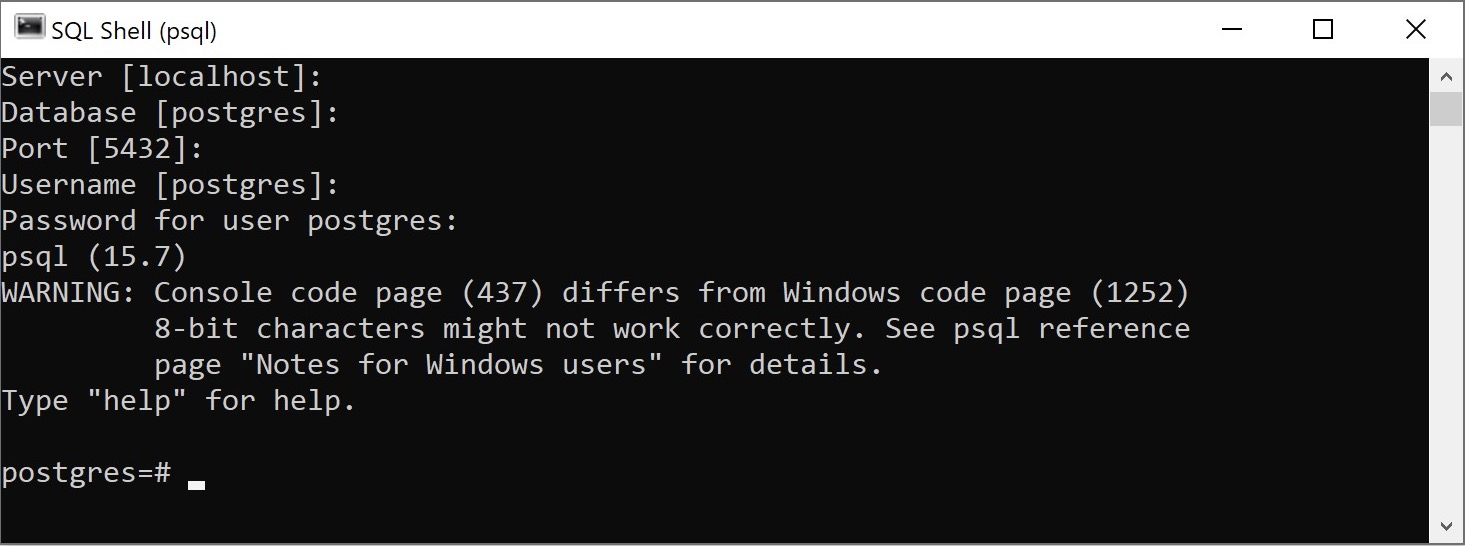
\includegraphics[width=.98\textwidth, trim={0mm 0mm 0mm 0.5mm},clip]{images/ch12/psqlconnect.jpg}};
  \drawshadow{image}
\end{tikzpicture}
\caption{psql မှ PostgreSQL ကို  စတင်ချိတ်ဆက်ပုံ} 
\label{fig:psqlconnect}
\end{figure}

\fEn{psql} ဖွင့်ပြီး စစချင်းမှာ ဒေတာဘေ့စ်နဲ့ ချိတ်ဆက်ဖို့ လိုအပ်တဲ့ အချက်အလက်တွေ ထည့်ပေးရပါမယ်။ ပုံ (\fRefNo{\ref{fig:psqlconnect}}) မှာ ကြည့်ပါ။ 
%
\begin{itemize}
\item \fEn{Server [localhost]:} (ချိတ်ဆက်မဲ့ ဆာဗာရဲ့ \fEn{Host Name/IP Address})
\item \fEn{Database [postgres]:} (ချိတ်ဆက်မဲ့ ဒေတာဘေ့စ်နံမည်)
\item \fEn{Port [5432]:} (\fEn{PostgreSQL port} နံပါတ်)
\item \fEn{Username [postgres]:} (ဒေတာဘေ့စ် ချိတ်ဆက်အသုံးပြုမဲ့ \fEn{user})
\item \fEn{Password for user postgres:} (ဒေတာဘေ့စ်ကို ချိတ်ဆက်အသုံးပြုမဲ့ \fEn{user} ရဲ့ \fEn{password})
\end{itemize}
%

လေးထောင့်ကွင်းထဲက \fEn{default} တန်ဖိုးတွေပါ။ တကူးတက ဘာမှမထည့်နေပဲ \fEn{Enter} နှိပ်ရင် အဲဒီတန်ဖိုးတွေ ထည့်တာနဲ့ တူတူပါပဲ။ စာမျက်နှာ \fRefNo{\pageref{apdx3}} နောက်ဆက်တွဲ (\fRefNo{\ref{apdx3}}) မှာ ဖော်ပြထားတဲ့အတိုင်း အင်စတောလ်လုပ်ထားတာဆိုရင် \fEn{password} တစ်ခုပဲ ထည့်ပေးဖို့လိုတယ်။ ကျန်တာက \fEn{default} အတိုင်းထားပြီး \fEn{Enter} နှိပ်သွားလို့ရတယ်။ \fEn{Password} က အင်စတောလ်လုပ်တုန်းက ပေးခဲ့တဲ့ \fEn{password} ကို ထည့်ပေးရမှာပါ။

\fEnBf{psql} ဆိုတာဘာလဲ။ \fEn{psql} ဟာ \fEn{PostgreSQL} ကို ချိတ်ဆက်အသုံးပြုဖို့ သုံးတဲ့ \fEn{command-line} ပရိုဂရမ်တစ်ခုပါ။ \fEn{Client} ပရိုဂရမ် အနေနဲ့ အသုံးပြုရတာပါ။ ဒေတာဘေ့စ် ချိတ်ဆက်ခြင်း၊ ဒေတာဘေ့စ်ဆီကို \fEn{SQL} ကွန်မန်းတွေ ပေးပို့လုပ်ဆောင်စေခြင်း၊ ဒေတာဘေ့စ် ပြန်ပို့ပေးတဲ့ ရလဒ်တွေပြပေးခြင်း၊ ဒေတာဘေ့စ် စီမံခန့်ခွဲခြင်း \fEn{(database administration)} စတဲ့ ကိစ္စတွေအတွက် အသုံးပြုနိုင်တယ်။ ရိုးရိုးရှင်းရှင်းပေမဲ့ အစွမ်းထက်တဲ့ \fEn{tool} တစ်ခုဖြစ်ပါတယ်။

\subsection*{ဒေတာဘေ့စ် အသစ်ဆောက်ခြင်း}
ဒေတာဘေ့စ် အသစ်တစ်ခု ဆောက်မယ်ဆိုရင် \fCode{CREATE DATABASE} \fEn{SQL} ကွန်မန်း သုံးပါတယ်။  
%
\begin{sql}
CREATE DATABASE ß\fEnEmp{database\_name}ß;
\end{sql}
%
\fEn{SQL language} ဟာ စာလုံး အကြီးအသေး မခွဲဘူး။ ဒီစာအုပ်မှာ \fEn{SQL keyword} တွေဆိုရင် အက္ခရာအကြီးနဲ့ ရေးပါမယ်။ \fEn{Database, table, column, function} စတာတွေရဲ့ နံမည် \fEn{(identifiers)} တွေက အက္ခရာအသေးနဲ့ ဖြစ်မယ်။
\fEn{student} ဒေတာဘေ့စ် အတွက် ဒီ \fEn{SQL} ကို
%
\begin{sql}
CREATE DATABASE students;
\end{sql}
%
\fEn{psql} ကနေ \fEn{run} ပေးပါ $\big\llbracket$ပုံ (\fRefNo{\ref{fig:createdb}})$\big\rrbracket$။ \fEn{SQL} စတိတ်မန့် တစ်ကြောင်း အဆုံးမှာ ဆီမီးကော်လံ \fEn{(\fCode{;})} ထည့်ပေးရပါမယ်။

\begin{figure}[tb!]
\begin{tikzpicture}
    \node[anchor=south west,inner sep=0] (image) at (0,0)
    {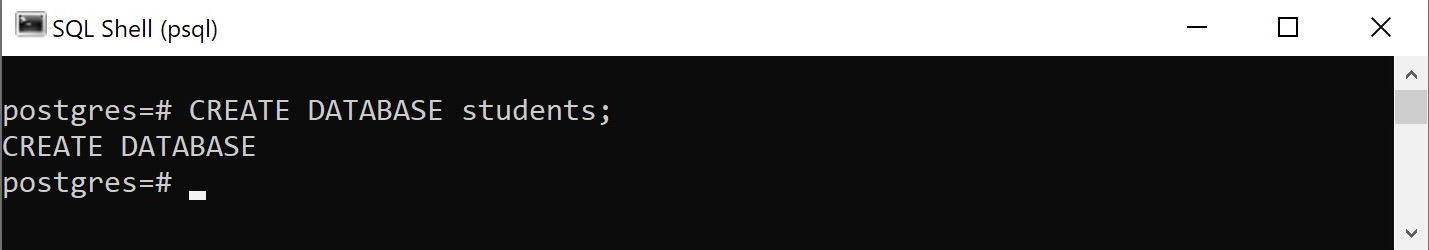
\includegraphics[width=.98\linewidth, trim={0mm, 0.5mm, 0.5mm, 0.5mm}, clip]{images/ch12/createdb.jpg}};
    \drawshadow{image}
\end{tikzpicture}
\caption{psql ကနေ ‘CREATE DATABASE’ SQL run တာ}
\label{fig:createdb}
\end{figure}

\fEn{psql} ကနေ \mintinline{text}|\l| (သို့) \mintinline{text}|\list| ကွန်မန်းနဲ့ \fEn{PostgreSQL} မှာ ရှိတဲ့ ဒေတာဘေ့စ်တွေကို ထုတ်ကြည့်နိုင်ပါတယ်။ ဒီလို \mintinline{text}|\| \fEn{(backslash)} နဲ့ စတဲ့ ကွန်မန်းတွေဟာ  \fEn{psql} သီးသန့်ဖြစ်တယ်။ \fEn{SQL} မဟုတ်တဲ့အတွက် \fEn{run} ရင် \fCode{;} မထည့်ရဘူး။ \mintinline{text}|\l| \fEn{run} လိုက်ရင် စာရင်းထဲမှာ \fEn{students} ဒေတာဘေ့စ် တွေ့ရမှာပါ $\big\llbracket$ပုံ (\fRefNo{\ref{fig:listdb}})$\big\rrbracket$။

\begin{figure}[htb!]
\begin{tikzpicture}
    \node[anchor=south west,inner sep=0] (image) at (0,0)
    {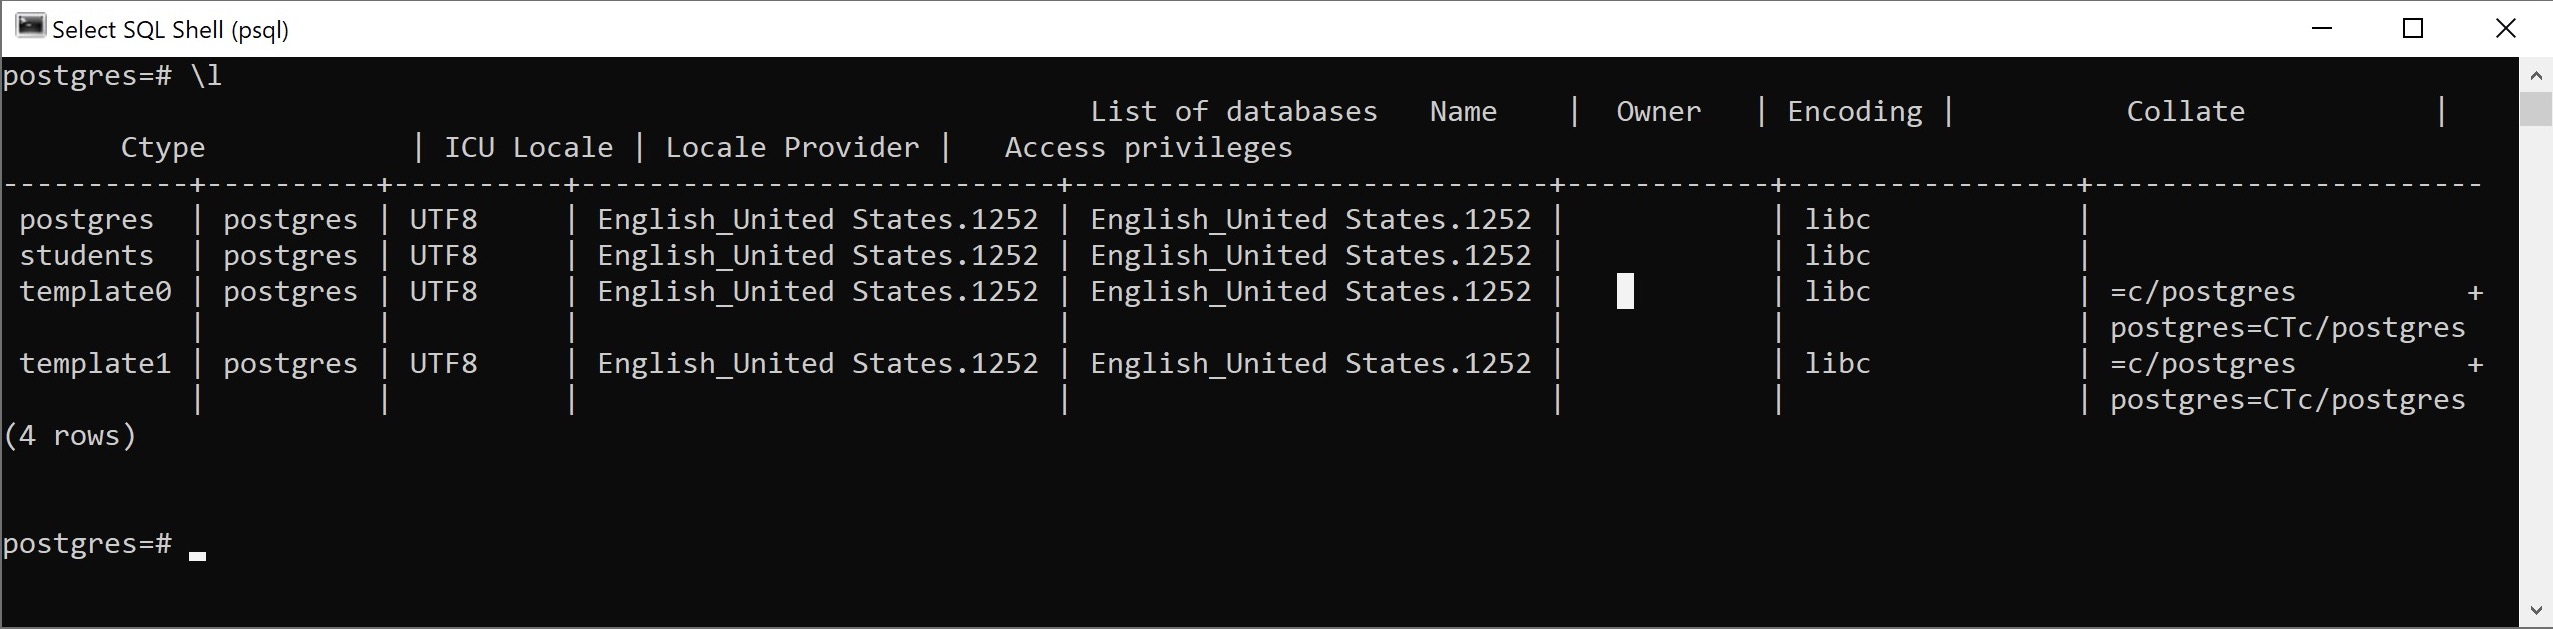
\includegraphics[width=.98\textwidth, trim={0mm 20mm 380mm 0.5mm},clip]{images/ch12/listdb.jpg}};
    \drawshadow{image}
\end{tikzpicture}
\caption{psql ကနေ ဒေတာဘေ့စ်တွေ list ထုတ်ကြည့်တာ}
\label{fig:listdb}
\end{figure}

\fEn{psql} မှာ ဒေတာဘေ့စ် ပြောင်းချိတ်မယ်ဆိုရင် \mintinline{text}|\c| (သို့) \mintinline{text}|\connect| နဲ့ ပြောင်းရပါမယ်။ \fEn{students} ဒေတာဘေ့စ်ကို အခုလို \fEn{connect} လုပ်ပါ
\begin{codetxt}
\c students
\end{codetxt}
\fEn{psql} က ဒီလို ပြပါလိမ့်မယ်
\begin{codetxt}
postgres=# \c students
You are now connected to database "students" as user "postgres".
students=#
\end{codetxt}

\begin{mytcbox}
\fEn{SQL} ကွန်မန်းကို \fEn{psql} က လုပ်ဆောင်ပေးတာ မဟုတ်ပါဘူး။ \fEn{psql} က \fEn{SQL} ကွန်မန်းကို ချိတ်ဆက်ထားတဲ့ ဒေတာဘေ့စ်ဆီ ပို့ပဲ ပို့ပေးတာ။ လက်ခံရရှိတဲ့ ဒေတာဘေ့စ်က အဲဒီ \fEn{SQL} ကို လုပ်ဆောင်ပေးတာပါ။ ဒီအချက်ကို ကွဲကွဲပြားပြား နားလည်ဖို့ လိုပါတယ်။
\end{mytcbox}

\subsection*{Table ဆောက်ခြင်း}
\fCode{CREATE TABLE} က \fEn{table} ဆောက်တဲ့ \fEn{SQL} ကွန်မန်းပါ။ \fEn{students} ဒေတာဘေ့စ်ထဲမှာ \fEn{student table} အောက်ပါအတိုင်း ဆောက်ပါမယ်
%
\begin{sql}
-- create a table named student 
CREATE TABLE student (
    id SERIAL PRIMARY KEY,
    name VARCHAR(100),
    age INT,
    grade VARCHAR(2)
);
\end{sql}
%  
\fEn{psql} မှာ \fEn{SQL} \fEn{run} ရင် လက်ရှိချိတ်ထားတဲ့ ဒေတာဘေ့စ်ကို အဲဒီ \fEn{SQL} ပေးပို့ လုပ်ဆောင်ခိုင်းပါတယ်။ အခုချိတ်ထားတာ \fEn{students} ဒေတာဘေ့စ်ဆိုတော့ \fEn{table} ကို အဲဒီ ဒေတာဘေ့စ်ထဲ ဆောက်ပေးသွားမှာပါ။ ဒီ \fEn{table} မှာ \fCode{id}\fEn{,} \fCode{name}\fEn{,} \fCode{age} နဲ့ \fCode{grade} \fEn{column} လေးခုရှိမယ်။ \fCode{--} ကို တစ်ကြောင်းတည်း ကွန်းမန့် အတွက် သုံးတယ်။ တစ်ကြောင်းထက်ပိုရင် \fCode{/*} နဲ့ ဖွင့် \fCode{*/} နဲ့ ပိတ် ရေးလေ့ရှိတယ်။ ဥပမာ
%
\begin{sql}
/* This is a
   multiline comment */
\end{sql}
%

\fEn{Column} တစ်ခုစီမှာ \fEn{data type} ရှိရပါမယ်။ \fCode{VARCHAR(100)} က အများဆုံး ကာရက်တာ အလုံးတစ်ရာ သိမ်းဆည်းနိုင်တယ်။ သိမ်းတဲ့ ကာရက်တာ အရေအတွက်ပေါ် မူတည်ပြီး နေရာယူတာ အနည်းအများ ကွာတယ်။ ငါခုသိမ်းရင် ငါးခုစာ၊ ဆယ်ခုသိမ်းရင် ဆယ်ခုစာပဲ နေရာကုန်မှာပါ။ အမြဲ အလုံး တစ်ရာစာ နေရာကုန်တာ မဟုတ်ဘူး။ \fCode{VARCHAR(2)} ဆိုရင် အများဆုံး  ကာရက်တာ နှစ်လုံး သိမ်းလို့ရမယ်။ \fEn{SQL} \fCode{VARCHAR} က \fEn{Python} \fCode{str} နဲ့ အလားတူတယ်။ \fCode{INT} ကတော့ \fEn{integer} ပါ။

\fCode{id} \fEn{column} က ထူးခြားပြီး နည်းနည်းပိုရှင်းပြဖို့ လိုတယ်။ \fCode{SERIAL} က \fEn{data type} အနေနဲ့ \fCode{INT} နဲ့ တူတူပဲ။ သူ့ရဲ့ ထူးခြားချက်က ဂဏန်းတွေကို အစဉ်အတိုင်း တစ်ခုပြီးတစ်ခု ထုတ်ပေးနိုင်တာပါ။ $1, 2, 3,\ldots$ စသည်ဖြင့်  နောက်ဆုံးတန်ဖိုးကို အလိုအလျောက် တစ်တိုးတိုးပြီး ထုတ်ပေးသွားမှာ ဖြစ်တယ်။ \fCode{id} \fEn{column} က \fEn{Primary Key} လည်းဖြစ်တယ်။ \fEn{Column} တစ်ခုကို \fEn{Primary Key} အဖြစ် ထားချင်ရင် \fCode{PRIMARY KEY} လို့ သတ်မှတ်ရပါမယ်။ \fEn{Primary Key} ဆိုရင် \fEn{column} တန်ဖိုး ထပ် \fEn{(duplicate)} လို့မရဘူး၊ \fEn{unique} ဖြစ်ရပါမယ်။ အခု သိပ်နားမလည်သေးရင်လည်း \fEn{table} မှာ ကျောင်းသား \fEn{record} တွေထည့်တာ ဆက်ကြည့်ရင် ကောင်းကောင်း နားလည်သွားမှာပါ။

\subsection*{\fSubSecCodeBf{INSERT}}
\fEn{Relational Data Model} အခြေခံတဲ့ \fEn{RDBMS} တွေဟာ ဒေတာတွေကို \fEn{table} ပုံစံနဲ့ သိမ်းဆည်းတယ်။ ကျောင်းသူ/သား တစ်ယောက်ချင်းစီအတွက် အချက်အလက်ကို \fEn{student table} မှာ  \fEn{row} တစ်ခုစီနဲ့ ထည့်သွင်း သိမ်းဆည်းပါမယ်။ \fEn{Row} ကို \fEn{record} လို့လည်း သုံးနှုန်းလေ့ရှိတယ်။ \fEn{Record} အသစ် ထည့်သွင်းမယ်ဆိုရင် \fEn{SQL} \fCode{INSERT} ကို သုံးရပါတယ်။

%
\begin{sql}
INSERT INTO student (name, age, grade) VALUES ('Amy', 20, 'A');
INSERT INTO student (name, age, grade) VALUES ('Kathy', 22, 'B');
INSERT INTO student (name, age, grade) VALUES ('Waiyan', 21, 'C');
\end{sql}
%

အေမီ၊ ကေသီ နဲ့ ဝေယံ ကျောင်းသား သုံးယောက်အတွက် \fEn{record} သုံးခု ထည့်သွင်းတာပါ။ \fEn{Column} နံမည်တွေ ဝိုက်ကွင်းထဲမှာ ထည့်ပြီး အဲ့ဒီ \fEn{column} တွေအတွက် တန်ဖိုးအသီးသီးကို အစဉ်အတိုင်း ထည့်ပေးရပါတယ်။ \fCode{age} နဲ့ \fCode{grade} ရှေ့နောက် ဖလှယ်လိုက်မယ်ဆိုရင် အခုလို
%
\begin{sql}
INSERT INTO student (name, grade, age) VALUES ('Amy', 'A',  20);
\end{sql}
%
\fEn{insert} လုပ်ရမှာပါ။

\fEn{student table} မှာ \fEn{column} က လေးခု ရှိတာပါ။ အခု \fCode{INSERT} တွေမှာကျတော့ သုံးခုပဲတွေ့ရပြီး \fCode{id} မပါဘူး။ ဘာကြောင့်ပါလဲ။ \fCode{INSERT} လုပ်တဲ့အခါ \fCode{SERIAL} \fEn{column} အတွက် တန်ဖိုးကို ဒေတာဘေ့စ်က အလိုအလျောက် ထည့်ပေးသွားတာ။ ကိုယ်တိုင်ထည့်ဖို့ မလိုဘူး။ ဒါကြောင့် \fCode{id} \fEn{column} ကို \fEnEmp{auto-incrementing} \fEn{primary key} \fEn{column} လို့ ခေါ်တယ်။ \fEn{Auto-increment} ဖြစ်ဖို့ အခြားနည်းလမ်းတွေလည်း ရှိပါတယ်။ \fCode{SERIAL} ကတော့ ဒီကိစ္စအတွက် လွယ်အောင် လုပ်ပေးထားတာပါ။ စောစောက \fCode{INSERT} သုံးကြောင်းကို \fEn{psql} မှာ \fEn{run} ပါ။ အေမီ၊ ကေသီ နဲ့ ဝေယံတို့အတွက် \fEn{record} အသီးသီးကို \fCode{id} နံပါတ် $1,2,3$ အစဉ်နဲ့ \fEn{student table} ထဲ ထည့်သွင်းသွားမှာဖြစ်တယ်။ နောက်ထပ် \fEn{record} တစ်ခု ထပ်ထည့်ရင် \fCode{id} နံပါတ် $4$ ဖြစ်မှာပါ။


\subsection*{\fSubSecCodeBf{SELECT}}
\fEn{Table} ဒေတာတွေ ထုတ်ယူကြည့်ဖို့ အသုံးပြုတဲ့ \fEn{SQL} ဖြစ်ပါတယ်။ \fEn{Student table} ထဲက \fEn{record} အားလုံးကို ကြည့်မယ်ဆို အခုလို 
%
\begin{sql}
SELECT id, name, age, grade FROM student;
\end{sql}
%
\fEn{Table} မှာ ရှိသမျှ \fEn{column} အကုန်လုံး ပါချင်ရင် \fCode{SELECT *} သုံးလို့လည်းရတယ်။ \fCode{SELECT *} ကို \fEn{‘Select All’} လို့ ဖတ်တယ်။
%
\begin{sql}
SELECT * FROM student;
\end{sql}
%

\begin{figure}[tbh!]
\begin{tikzpicture}
  \node[anchor=south west,inner sep=0] (image) at (0,0)
  {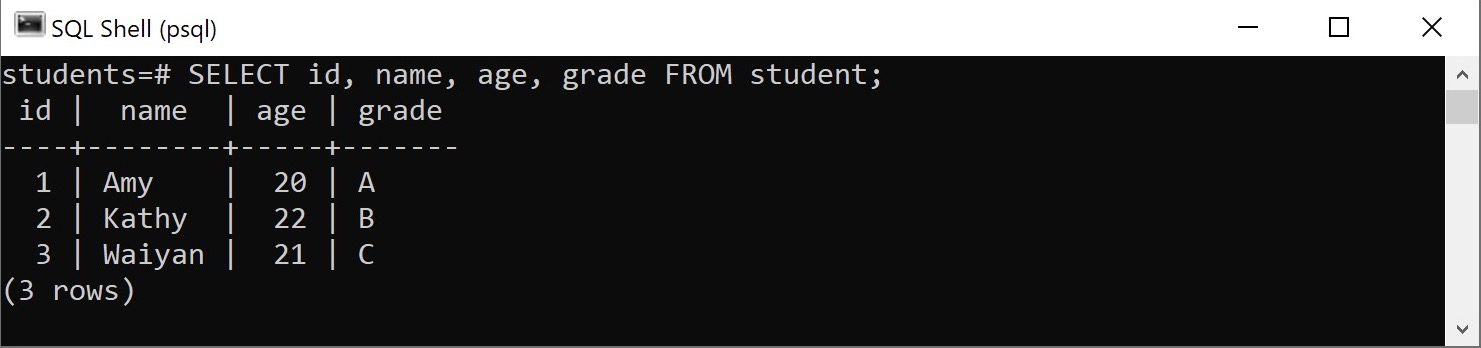
\includegraphics[width=.98\textwidth, trim={0mm 0.5mm 0.5mm 0.2mm}]{images/ch12/select.jpg}};
  \drawshadow{image}
\end{tikzpicture}
\caption{psql ကနေ select လုပ်တာ} 
\label{fig:selectstu}
\end{figure}

\fEn{Column} အကုန်မထုတ်ဘဲ ကိုယ်လိုချင်တာပဲ ရွေးပြီး \fEn{select} လုပ်ချင်လည်း ရတယ်။ အောက်ပါတို့ကို \fEn{psql} မှာ စမ်းကြည့်ပါ။
%
\begin{sql}
SELECT name, grade FROM student;
SELECT name, age, id FROM student;
\end{sql}
%
\subsection*{\fSubSecCodeBf{WHERE}}
\fEn{Grade A} ရတဲ့ ကျောင်းသားတွေကိုပဲ ရွေးထုတ်ကြည့်မယ် ဆိုပါစို့။ ဒီအတွက် \fEn{SQL} မှာ \fCode{WHERE} ရှိပါတယ်။ ဥပမာ
%
\begin{sql}
SELECT * FROM student WHERE grade = 'A';
\end{sql}
%
\fCode{WHERE} နောက်မှာ ဘူလီယန် အိပ်စ်ပရက်ရှင်တစ်ခု လိုက်ရပါမယ်။ \fCode{WHERE} ကွန်ဒီရှင် \fEn{(Condition)} လို့ခေါ်တယ်။ ရေးပုံရေးနည်း နည်းနည်းကွာပေမဲ့ \fEn{SQL} \fCode{WHERE} ကွန်ဒီရှင် က \fEn{Python} ဘူလီယန် အိပ်စ်ပရက်ရှင်နဲ့ သဘောတရားအားဖြင့် တူပါတယ်။ \fCode{grade = 'A'} က \fCode{grade} \fEn{column} တန်ဖိုး \fCode{'A'} နဲ့ ညီလား စစ်တာ။ ညီတဲ့ \fEn{record} တွေကိုပဲ \fCode{WHERE} က စစ်ထုတ်ပေးမှာပါ။ ဒါ့ကြောင့် အပေါ်က \fCode{select} က \fEn{record} တစ်ကြောင်းပဲ ထွက်မှာပါ။ အေမီတစ်ယောက်ပဲ \fEn{A} ရပါတယ်။ \fCode{WHERE} နဲ့ပါတ်သက်ပြီး လက်တွေ့စမ်းကြည့်ရအောင် အောက်ပါအတိုင်း ကျောင်းသား \fEn{record} လေးခု ထပ်ထည့်ပါမယ်။  
%
\begin{sql}
INSERT INTO student (name, age, grade) VALUES ('Sandy', 19, 'A');
INSERT INTO student (name, age, grade) VALUES ('Thida', 21, 'B');
INSERT INTO student (name, age, grade) VALUES ('Peter', 21, 'B');
INSERT INTO student (name, age, grade) VALUES ('Haymar', 18, NULL);
\end{sql}
%

\fEn{Grade A} သို့ \fEn{B} ရတဲ့ ကျောင်းသား \fEn{record} တွေ \fEn{select} လုပ်ဖို့ \fCode{OR} သုံးထားတာပါ။ \fEn{psql} မှာ စမ်းကြည့်ပါ။ \fEn{Amy, Kathy, Sandy, Thida, Peter} တို့ \fEn{A} သို့ \fEn{B} ရကြတယ်။
%
\begin{sql}
SELECT * FROM student WHERE grade = 'A' OR grade = 'B';
\end{sql}
\fEn{Grade A} သို့ \fEn{B} မရတဲ့ ကျောင်းသားတွေ ထုတ်ချင်ရင် \fCode{NOT} နဲ့ အခုလို ရတယ်
%
\begin{sql}
SELECT name FROM student WHERE NOT(grade = 'A' OR grade = 'B');
\end{sql}
ဝေယံ တစ်ယောက်ပဲ ရလဒ်မှာတွေ့ရမှာပါ။ ဟေမာ ဘာကြောင့် မပါရတာလဲ။ စဉ်းစားကြည့်ရင် သူမ \fEn{A} လည်းမရ၊ \fEn{B}  လည်းမရဘူး။ ဒါကြောင့်  ပါသင့်တယ် ယူဆကောင်း ယူဆနိုင်တယ်။ \fCode{NULL} ဟာ မရှိခြင်း၊ မသိခြင်း ကိုဖော်ပြဖို့ \fEn{SQL} မှာ အသုံးပြုတဲ့ \fEn{special value} တစ်ခု ဖြစ်ပါတယ်။ ဟေမာ့ \fEn{grade} က \fCode{NULL} ဖြစ်နေတယ်။ ဆိုလိုတာက သူ့ \fEn{grade} ကို မသိဘူး။ 

\fCode{NULL} နဲ့ အခြားတန်ဖိုးတစ်ခုခု ညီ/မညီ စစ်တဲ့အခါ ရလဒ်က \fCode{NULL} ပဲ ဖြစ်ပါတယ်။ အဓိပ္ပါယ်က ညီ/မညီ ‘မသိဘူး’ ဆိုတဲ့ အဓိပ္ပါယ်။ ဒါ့ကြောင့် ဘူလီယန် အိပ်စ်ပရက်ရှင် \fCode{'A' = NULL} ရဲ့ အဖြေ \fCode{NULL} ဖြစ်သလို \fCode{'A' <> NULL} ရဲ့ အဖြေလည်း \fCode{NULL} ပဲ ဖြစ်တယ်။ \fCode{<>} က မညီဘူးလား စစ်တာ၊ \fCode{=} နဲ့ ပြောင်းပြန်။ 

\fEn{Select} လုပ်တဲ့အခါ \fCode{WHERE} ကွန်ဒီရှင် \fEn{true} ဖြစ်တဲ့ \fEn{record} တွေကို ရွေးထုတ်ပေးတယ်။ \fCode{WHERE} ကွန်ဒီရှင် ရလဒ်တန်ဖိုး \fCode{NULL} ဖြစ်ရင် အဲဒီ \fEn{record} ကို ထုတ်ပေးမှာ မဟုတ်ဘူး။ စောစောက \fEn{select} ရလဒ်မှာ ဟေမာ ဘာ့ကြောင့်  မပါလဲ အောက်ပါအတိုင်း စဉ်းစားကြည့်နိုင်ပါတယ်%
%
\[
\begin{aligned}
         &\text{\fEn{WHERE NOT(\textit{NULL} = \`{}A\`{} OR \textit{NULL} = \`{}B\`{})}}\\
\implies &\text{\fEn{WHERE NOT(\textit{NULL} OR \textit{NULL})}}\\
\implies &\text{\fEn{WHERE NOT(\textit{NULL})}}\\
\implies &\text{\fEn{WHERE \textit{NULL}}}\\
\end{aligned}%
\]
\fEn{Grade C} မဟုတ်တဲ့ ကျောင်းသားတွေကို အောက်ပါအတိုင်း နည်းလမ်းနှစ်မျိုးနဲ့ \fEn{select} လုပ်ကြည့်ပါ။ အခုတစ်ခါလည်း ဟေမာ ရလဒ်မှာ မပါတာကို သတိပြုပါ။
%
\begin{sql}
SELECT * FROM student WHERE grade <> 'C';
\end{sql}
%
%
\begin{sql}
SELECT * FROM student WHERE NOT(grade = 'C');
\end{sql}
%
ဒီတစ်ခု ထပ်စမ်းကြည့်ပါ။ ရှင်းပြဖို့မလိုဘဲ အဓိပ္ပါယ် နားလည်မယ် ထင်ပါတယ်။
%
\begin{sql}
SELECT * FROM student WHERE grade = 'B' AND id <= 5;
\end{sql}
%

\fCode{NULL} ဟုတ်/မဟုတ် စစ်ချင်ရင် \fEn{SQL} မှာ \fCode{IS NULL} (သို့) \fCode{IS NOT NULL}  သုံးရပါတယ်။ \fCode{=} နဲ့ \fCode{<>} ကို သုံးလို့မရဘူး။ မှားယွင်း အသုံးပြုမိတတ်လို့ ဒီအချက်ကို အထူးဂရုပြုရပါမယ်။ \fEn{Grade} \fCode{NULL} ဖြစ်တဲ့ \fEn{record} တွေနဲ့ \fCode{NULL} မဟုတ်တဲ့ \fEn{record} တွေကို အခုလို ရွေးထုတ်နိုင်ပါတယ်။
%
\begin{sql}
SELECT * FROM student WHERE grade IS NULL;
SELECT * FROM student WHERE grade IS NOT NULL;
\end{sql}
%
\fEn{Grade} \fCode{NULL} ဖြစ်တာ ဟေမာတစ်ယောက်ပဲ ရှိတာမို့လို့ ပထမ \fEn{select} က \fEn{record} တစ်ကြောင်းပဲ ထွက်မှာပါ။ အောက်ပါအတိုင်း တစ်ဆင့်ချင်း စဉ်းစားကြည့်ပါ
\[
\begin{aligned}
    &\text{\fEn{WHERE grade IS \textit{NULL}}}\\
\implies &\text{\fEn{WHERE \textit{NULL} IS \textit{NULL}}}\\
\implies &\text{\fEn{WHERE TRUE}}\\
\end{aligned}
\]
ဒုတိယ \fEn{select} မှာ ကျတော့ ဘာကြောင့် ဟေမာ မပါလဲ။ ကျန်တဲ့သူတွေကရော ဘာကြောင့်ပါလဲ။ အောက်ပါအတိုင်း တစ်ဆင့်ချင်း စဉ်းစားကြည့်ပါ။ ဟေမာ့ \fEn{record} အတွက်%
%
\[
\begin{aligned}
    &\text{\fEn{WHERE grade IS NOT \textit{NULL}}}\\
\implies &\text{\fEn{WHERE \textit{NULL} IS NOT \textit{NULL}}}\\
\implies &\text{\fEn{WHERE FALSE}}\\
\end{aligned}
\]
\fEn{A} ရထားတဲ့ ကျောင်းသား \fEn{record} ဆိုရင် ဒီလို
\[ 
\begin{aligned}
    &\text{\fEn{WHERE grade IS NOT \textit{NULL}}}\\
\implies &\text{\fEn{WHERE \`{}A\`{} IS NOT \textit{NULL}}}\\
\implies &\text{\fEn{WHERE TRUE}}\\
\end{aligned}
\]
အခြား \fCode{NULL} မဟုတ်တဲ့ \fEn{grade} အားလုံးအတွက် အလားတူဖြစ်မယ်။ ဒါ့ကြောင့် ဒုတိယ \fEn{select} ရလဒ်မှာ ဟေမာကလွဲလို့ ကျန်တဲ့သူအားလုံး ပါလာတာဖြစ်တယ်။

\subsection*{\fSubSecCodeBf{ORDER BY}}
\fCode{ORDER BY} က \fEn{record} တွေကို \fEn{column} တန်ဖိုးပေါ် မူတည်ပြီး ‘အစဉ်အတိုင်းစီခြင်း’ \fEn{(sorting)} အတွက်ပါ။
%
\begin{sql}
SELECT * FROM student ORDER BY grade;
\end{sql}
%
\fEn{Grade} အလိုက် \fEn{order by} လုပ်ထားတာပါ။ ရလဒ်ကို ပုံ (\fRefNo{\ref{fig:orderbyasc}}) မှာ ကြည့်ပါ။ ကြီးစဉ်ငယ်လိုက် စီချင်ရင် \fCode{DESC} \fEn{(descending)} နဲ့ ရတယ်။
\begin{figure}[tbh!]
\begin{tikzpicture}
  \node[anchor=south west,inner sep=0] (image) at (0,0)
  {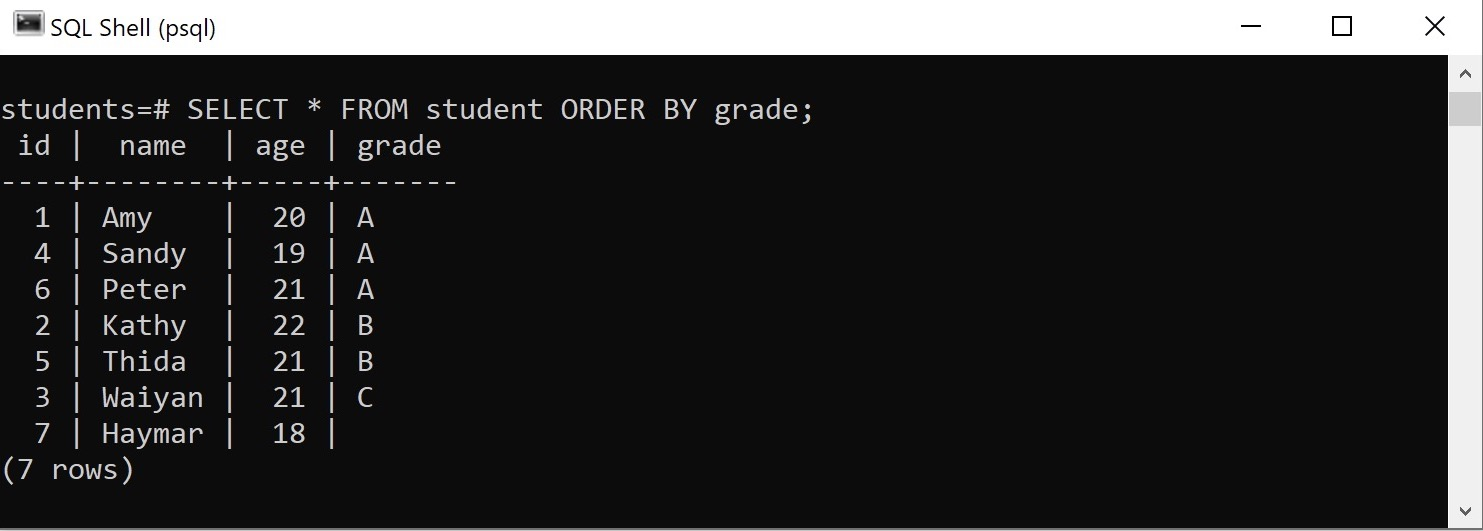
\includegraphics[width=.98\textwidth, trim={0mm 0.5mm 0.5mm 0.5mm},clip]{images/ch12/orderbyasc.jpg}};
  \drawshadow{image}
\end{tikzpicture}
\caption{order by နဲ့ grade အလိုက် စီထားတာ} 
\label{fig:orderbyasc}
\end{figure}
%
\begin{sql}
SELECT * FROM student ORDER BY grade DESC;
\end{sql}
%
သူ့ နဂို \fEn{default} ကတော့ \fCode{ASC} \fEn{(ascending)} ပါ။ 

\fEn{Column} တစ်ခုမကနဲ့  စီချင်လည်း ရတယ်။ \fCode{ORDER BY} နောက်မှာ \fEn{sort} လုပ်ရမဲ့ \fEn{column} တွေ ထည့်ပေးရုံပဲ။ \fEn{Age} နဲ့ \fEn{grade} တွဲရက် \fEn{sort} လုပ်မယ်ဆိုရင်
%
\begin{sql}
SELECT * FROM student ORDER BY age, grade;
\end{sql}
%
\fEn{psql} ရလဒ်မှာ အောက်ပါအတိုင်း တွေ့ရမှာပါ။ \fEn{Thida, Peter, Waiyan} တို့ကို သေချာ ဂရုပြုကြည့်ပါ။ \fEn{Age} တူရင် \fEn{grade B} ရတဲ့သူက အရင်လာတာကို တွေ့ရပါမယ်။ \fEn{Grade C} က နောက်မှာပါ။
\begin{vbtm}
ß\fEnBf{Output:}ß
 id |  name  | age | grade
----+--------+-----+-------
  7 | Haymar |  18 |
  4 | Sandy  |  19 | A
  1 | Amy    |  20 | A
  5 | Thida  |  21 | B
  6 | Peter  |  21 | B
  3 | Waiyan |  21 | C
  2 | Kathy  |  22 | B
(7 rows)
\end{vbtm}
\fEn{Name} ထပ်ထည့်ကြည့်ပါ။  \fEn{Peter} က \fEn{Thida} ရဲ့ ရှေ့ရောက်သွားတာကလွဲလို့ ခုနက စီထားတာနဲ့ အားလုံးတူပါမယ်။
%
\begin{sql}
SELECT * FROM student ORDER BY age, grade, name;
\end{sql}
%

\fEn{Age} နဲ့ \fEn{grade} ကို ရှေ့‌နောက် ပြောင်းကြည့်ပါ။ 
%
\begin{sql}
SELECT * FROM student ORDER BY grade, age;
\end{sql}
%
\fEn{Grade} \fEn{A, B, C} အစဉ်အတိုင်း ဖြစ်မယ်။ \fEn{Grade} တူရင်တော့ \fEn{age} ငယ်တဲ့ \fEn{record} က ရှေ့ရောက်ပါတယ်။ အခုလို စီသွားမှာပါ
%
\begin{vbtm}
ß\fEnBf{Output:}ß
 id |  name  | age | grade
----+--------+-----+-------
  4 | Sandy  |  19 | A
  1 | Amy    |  20 | A
  5 | Thida  |  21 | B
  6 | Peter  |  21 | B
  2 | Kathy  |  22 | B
  3 | Waiyan |  21 | C
  7 | Haymar |  18 |
(7 rows)
\end{vbtm}
%

\fEn{Grade} ကို \fCode{DESC} နဲ့ \fEn{age} ကို \fCode{ASC} ထားကြည့်ပါ။ ခုနကဟာနဲ့ ဘာကွာခြားလဲ သေချာဂရုပြု လေ့လာကြည့်ပါ။
%
\begin{sql}
SELECT * FROM student ORDER BY grade DESC, age ASC;
\end{sql}
%
\begin{vbtm}
ß\fEnBf{Output:}ß
 id |  name  | age | grade
----+--------+-----+-------
  7 | Haymar |  18 |
  3 | Waiyan |  21 | C
  6 | Peter  |  21 | B
  5 | Thida  |  21 | B
  2 | Kathy  |  22 | B
  4 | Sandy  |  19 | A
  1 | Amy    |  20 | A
(7 rows)
\end{vbtm}

\fCode{ORDER BY} နဲ့ စီတဲ့အခါ \fCode{ORDER BY} နောက်မှာ \fEn{list} လုပ်ထားတဲ့ \fEn{column} အစီအစဉ်နဲ့ \fCode{ASC}\fEn{,} \fCode{DESC} တို့ကို လိုသလို အသုံးပြုပြီး လိုချင်တဲ့အတိုင်း ရအောင် \fEn{sort} လုပ်လို့ရပါတယ်။ ပရိုဂရမ်းမင်းမှာရော ဒေတာဘေ့စ်ပိုင်းမှာပါ \fEn{sorting} စီခြင်းဟာ အရေးကြီးတာကြောင့် ကျွမ်းကျင်အောင် လုပ်ထားသင့်ပါတယ်။


\subsection*{\fSubSecCodeBf{UPDATE}}
\fEn{Table record} တွေ \fEn{update} လုပ်ဖို့ အသုံးပြုတဲ့ \fEn{SQL} စတိတ်မန့် ဖြစ်ပါတယ်။ \fCode{id} နံပါတ် \fEn{7} နဲ့ \fEn{record} ရဲ့ \fEn{grade} နဲ့ \fEn{age} ကို \fEn{update} လုပ်မယ်ဆိုရင် ဒီလို
%
\begin{sql}
UPDATE student SET grade = 'A', age = 19 WHERE id = 7;
\end{sql}
%
\fCode{WHERE} ပါရင် \fCode{WHERE} ကွန်ဒီရှင်နဲ့ ကိုက်ညီတဲ့ \fEn{record} ကိုပဲ \fEn{update} လုပ်တယ်။ အခု \fEn{update} စတိတ်မန့်က \fCode{id} \fEn{7} နဲ့ က ဟေမာ့ \fEn{record} တစ်ခုကိုပဲ \fEn{update} လုပ်မှာပါ။ အကယ်၍ \fCode{WHERE} မပါခဲ့ရင် \fEn{table} မှာရှိတဲ့ \fEn{record} တွေ အကုန်လုံးကို \fEn{update} လုပ် သွားလိမ့်မယ်။

%
\begin{sql}
UPDATE student SET grade = 'A+' WHERE id IN (1, 4, 6);
\end{sql}
%
\fCode{id} နံပါတ်က $(1,4,6)$ ထဲမှာပါရင် \fEn{grade} ကို \fEn{A+} \fEn{update} လုပ်ထားတာပါ။ \fCode{WHERE} ကွန်ဒီရှင်မှာ \fCode{IN}  အော်ပရိတ်တာ သုံးထားတယ်။ \fEn{Column} တစ်ခုရဲ့ တန်ဖိုးဟာ \fEn{list} လုပ်ထားတဲ့ တန်ဖိုးတွေထဲမှာ ပါ/မပါ စစ်ချင်ရင် \fCode{IN} သုံးပါတယ်။ \fEn{Update} လုပ်ထားတဲ့ \fEn{record} တွေကို \fEn{select} လုပ်ကြည့်ပါ။ 
%
\begin{sql}
SELECT * FROM student WHERE id IN (1, 4, 6, 7);
\end{sql}
%
ပုံ (\fRefNo{\ref{fig:afterupdate}}) မှာလို တွေ့ရပါမယ်။

\begin{figure}[tbh!]
\begin{tikzpicture}
  \node[anchor=south west,inner sep=0] (image) at (0,0)
  {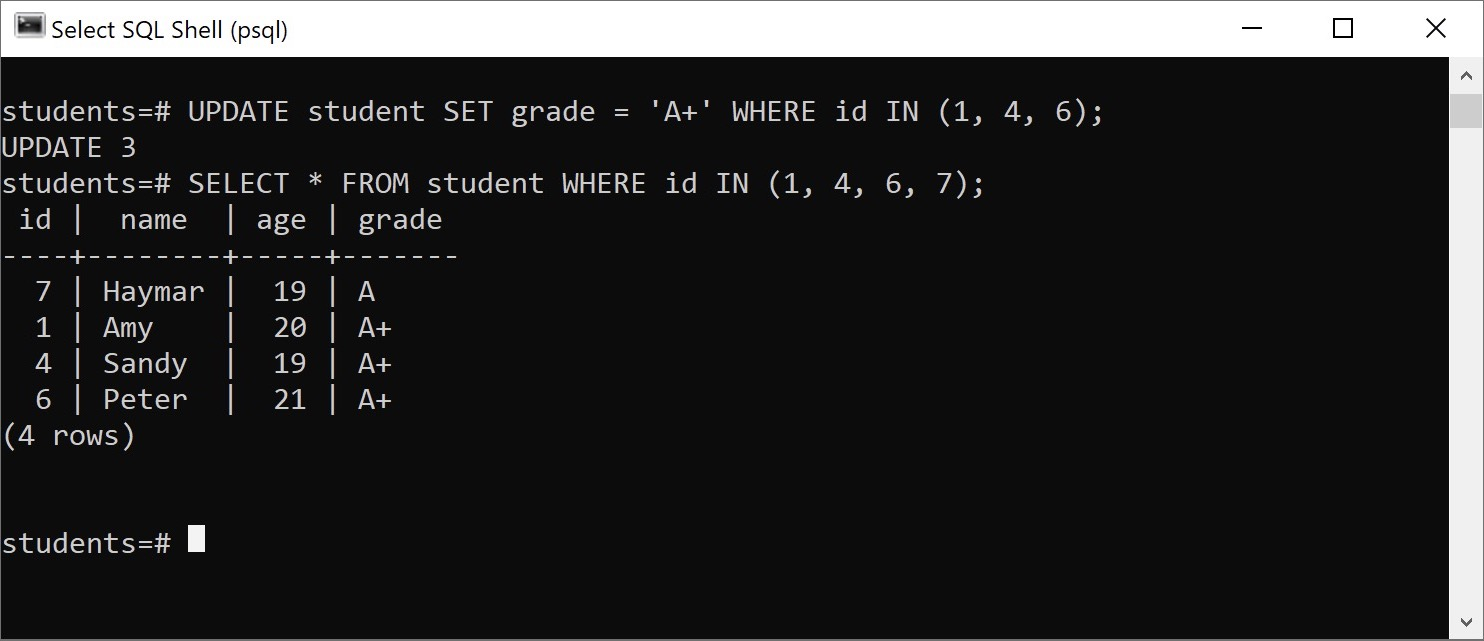
\includegraphics[width=.98\textwidth, trim={0mm 50mm 0.5mm 0.5mm},clip]{images/ch12/afterupdate.jpg}};
  \drawshadow{image}
\end{tikzpicture}
\caption{record တချို့ကို update လုပ်ပြီးနောက် select ပြန်လုပ်ကြည့်တာ} 
\label{fig:afterupdate}
\end{figure}

\subsection*{\fSubSecCodeBf{DELETE}}
\fEn{Table row} တွေ ဖျက်ဖို့ အသုံးပြုတဲ့ စတိတ်မန့် ဖြစ်ပါတယ်။ \fEn{Student table} ထဲက \fEn{record} အားလုံး ဖျက်မယ်ဆိုရင် အခုလို ဖျက်ရမှာပါ
%
\begin{sql}
DELETE FROM students;
\end{sql}
%
\fEn{Development/testing} ဒေတာဘေ့စ်မှာ \fEn{table} ဒေတာ အကုန်ဖျက်ပြီး အစမ်းဒေတာ \fEn{(test data)} ပြန်ထည့်ဖို့ ဒီလို လုပ်ရလေ့ရှိပေမဲ့ တကယ်သုံးနေတဲ့ \fEn{production} ဒေတာဘေ့စ်မှာတော့ \fEn{table} ဒေတာ အကုန်ဖျက်ပစ်ရမဲ့ အခြေအနေဆိုတာ ကြုံတောင့်ကြုံခဲပါပဲ။ ဖျက်ရမဲ့ \fEn{record} ကို \fCode{WHERE} နဲ့ရွေး ဖျက်တာက ပိုပြီး သဘာဝကျပါတယ်။ ဝေယံ ကျောင်းထွက်သွားလို့ သူ့ \fEn{record} ကို သိမ်းထားဖို့ မလိုတော့ဘူး ဆိုပါစို့၊ အခုလို \fEn{delete} လုပ်နိုင်ပါတယ် 
%
\begin{sql}
DELETE FROM student WHERE id = 3; -- id 3 is Waiyan
\end{sql}
%


\section{Table Relationships}
ဒေတာဘေ့စ် တစ်ခုမှာ \fEn{table} တစ်ခုမက \fEn{(multiple tables)} ပါဝင် ဖွဲ့စည်းထားလေ့ ရှိတယ်။ \fEn{Table} တွေနဲ့ ၎င်းတို့ကြား \fEnEmp{relationship} ဟာ \fEn{Relational Data Model} ရဲ့ အဓိကကျတဲ့ သဘောတရားဖြစ်တယ်။ သက်ဆိုင်\allowbreak ရာ \fEn{table} အသီးသီးမှာ အချက်အလက်တွေ စုစည်းသိမ်းဆည်းပုံ သိမ်းဆည်းနည်း စနစ်ကို လေ့လာကြရအောင်။ 

ဘဏ်တစ်ခုကို စိတ်ကူးကြည့်ပါ။ ဘဏ်အကောင့်၊ အကောင့်ပိုင်ရှင်နဲ့ ငွေဝင်ငွေထွက် စာရင်း အချက်\allowbreak အလက်တွေ သိမ်းဆည်းမယ် ဆိုပါစို့။ \fEn{Table} တစ်ခုတည်းနဲ့ အားလုံးသိမ်းလို့ ရပေမဲ့ \fEn{Relational Data Model} အရ \fEn{table} သုံးခုခွဲပြီး သီးခြားစီသိမ်းတာ ပိုကောင်းပါတယ်။  အကောင့်ပိုင်ရှင်နဲ့ သက်ဆိုင်တဲ့ အချက်အလက်တွေအတွက် \fEn{table} တစ်ခု ရှိပါမယ်။
%
\begin{sql}
CREATE TABLE account_holder (
    holder_id SERIAL PRIMARY KEY,
    fname VARCHAR(50),
    lname VARCHAR(50),
    dob DATE,
    address TEXT
);
\end{sql}
%
အခု \fEn{table} တွေကို ဒေတာဘေ့စ် အသစ်တစ်ခုထဲမှာထားတာ ပိုသင့်တော်မယ်။ (ကျောင်းသား ကိစ္စနဲ့ဆိုင်တဲ့ \fEn{table} တွေကို \fEn{students} ဒေတာဘေ့စ်၊ ဘဏ်နဲ့သက်ဆိုင်တာကို \fEn{bank} ဒေတာဘေ့စ် သတ်သတ်စီခွဲထားရင် ပိုပြီး စနစ်ကျတာကြောင့်ပါ။ အစမ်းလေ့လာတာမို့ သိပ်တော့ အရေးမကြီးပါ)။ \fEn{psql} မှာ အောက်ပါအတိုင်း တစ်ကြောင်းချင်း \fEn{run} ပါ
\begin{vbtm}
\c postgres
CREATE DATABASAE bank;
\c bank
\end{vbtm}
ပြီးတော့မှ \fCode{account\_holder} \fEn{table} အတွက် အပေါ်က \fCode{CREATE TABLE} ကို ဆက် \fEn{run} ပါ။ အခုချိတ်ထားတာက \fCode{bank} ဒေတာဘေ့စ် (\mintinline{text}|\c bank| \fEn{run} ထားတာ သတိပြုပါ)၊ ဆိုတော့ \fEn{table} က အဲဒီထဲမှာ ဆောက်မှာပါ။

အကောင့်နဲ့ သက်ဆိုင်တဲ့ အချက်အလက်တွေအတွက် \fEn{table} တစ်ခု ထပ်ဆောက်ပါမယ်။ (အခု \fEn{table} နှစ်ခုကို အရင်ကြည့်ရအောင်၊ ငွေဝင်ငွေထွက် စာရင်းနဲ့ ဆိုင်တဲ့ တတိယ \fEn{table} ကို နောက်ပိုင်းမှာ တွေ့ရမှာပါ)။ 
%
\begin{sql}
CREATE TABLE account (
    acc_id SERIAL PRIMARY KEY,
    /* ß\fMM{အခု}ß holder_id ß\fMM{က}ß account_holder ß\fEn{table} \fMM{ရဲ့}ß holder_id ß\fMM{ကို}ß 
    ß\fEn{reference} \fMM{လုပ်ထားတယ်}ß */ 
    holder_id INT REFERENCES account_holder(holder_id),
    acc_no VARCHAR(20) UNIQUE,
    acc_type VARCHAR(20),
    balance NUMERIC(12, 2) DEFAULT 0.00
);
\end{sql}
%

\fCode{account} \fEn{table} မှာ \fCode{holder\_id} \fEn{column} က \fCode{account\_holder} \fEn{table} ရဲ့ \fCode{holder\_id} \fEn{column} ကို ရည်ညွှန်းထားပါတယ်။ အကောင့်နဲ့ အကောင့် ပိုင်ရှင် အချက်အလက်တွေကို ဒီ \fEn{table} နှစ်ခုမှာ ဘယ်လို ဆက်စပ် သိမ်းဆည်းလဲ နားလည်အောင် နမူနာ \fEn{record} အနည်းငယ်ထည့်ပြီး ရှင်းပြပါမယ်။ အောက်ပါအတိုင်း \fEn{insert} လုပ်ပါ။
%
\begin{sql}
INSERT INTO account_holder (fname, lname, dob, address)
VALUES 
('Amy', 'Moe', '1985-02-15', '123 Main St, Sanchaung'),
('Sandy', 'Soe', '1990-06-23', '456 Oak St, Kamayaut');
\end{sql}
%
\fEn{Insert} လုပ်ပြီးရင် အေမီနဲ့ စန္ဒီ့ \fCode{holder\_id} နံပါတ်က $1$ နဲ့ $2$ အသီးသီး ဖြစ်မယ်။ အေမီဖွင့်ထားတဲ့ အကောင့်နှစ်ခုနဲ့ စန္ဒီရဲ့ အကောင့်တစ်ခုကို အောက်ပါအတိုင်း \fCode{account} \fEn{table} မှာ သိမ်းနိုင်ပါတယ်။ \fCode{holder\_id} $1$ နဲ့ $2$ ကို အထူး ဂရုပြုပါ။
%
\begin{sql}
INSERT INTO account (holder_id, acc_no, acc_type, balance)
VALUES 
(1, '0086-6002-1111', 'Savings', 500000.00),
(1, '0088-6005-1122', 'Current', 800000.00),
(2, '0086-6002-3311', 'Savings', 400000.00);
\end{sql}
%
ဒီ \fEn{table} မှာ ကြည့်ရင် အကောင့်ပိုင်ရှင် အသေးစိတ်အချက်အလက်ကို မတွေ့ရပါဘူး။ အကောင့် \fEn{record} တစ်ခုစီအတွက်  ပိုင်ရှင်ရဲ့ \fCode{holder\_id} ကိုပဲ တွေ့ရမှာပါ။ ဒီ \fCode{holder\_id} ဟာ \fCode{account\_holder} \fEn{table} ထဲက \fEn{record} တစ်ခုရဲ့ \fCode{holder\_id} ကို ရည်ညွှန်းရပါမယ်။ 

ပထမ အကောင့်နှစ်ခု \fCode{holder\_id} က $1$ ဖြစ်တယ်။ \fCode{account\_holder} \fEn{table} မှာပြန်ကြည့်ရင် \fCode{holder\_id} $1$ က အေမီ။ ဒါကြောင့် ဒီအကောင့်နှစ်ခုဟာ အေမီ့ရဲ့ အကောင့်ဖြစ်တယ်။ ထိုနည်းတူစွာ \fCode{holder\_id} $2$ က စန္ဒီဖြစ်တဲ့အတွက် တတိယအကောင့်ဟာ သူမရဲ့ အကောင့်ဖြစ်တယ်လို့ သိနိုင်ပါတယ်။ အခု ဖော်ပြခဲ့သလို အချက်အလက် သိမ်းဆည်းပုံ နည်းစနစ်ဟာ \fEn{Relational Model} ရဲ့ အဓိကကျတဲ့ အခြေခံ သဘောတရားလို့ ဆိုရမှာပါ။

\subsection*{Table \fSubSecCodeBf{JOIN}}
\fEn{Table} နှစ်ခုကို ပေါင်းစပ်ကြည့်ရင် အကောင့်ရော အကောင့်ပိုင်ရှင် အချက်အလက်ကိုပါ အပြည့်အစုံ သိနိုင်မှာပါ။ ဥပမာ အခုလို \fEn{select} လုပ်ကြည့်ရင် အေမီနဲ့ သူမ၏အကောင့် အသေးစိတ် အချက်အလက်တွေကို တွေ့ရပါမယ်
%
\begin{sql}
SELECT * FROM account_holder WHERE holder_id = 1;
SELECT * FROM account WHERE holder_id = 1;
\end{sql}
%
\begin{vbtm}
ß\fEnBf{Output:}ß
 holder_id | fname | lname |    dob     |        address
-----------+-------+-------+------------+------------------------
         1 | Amy   | Moe   | 1985-02-15 | 123 Main St, Sanchaung
(1 row)


 acc_id | holder_id |     acc_no     | acc_type |  balance
--------+-----------+----------------+----------+-----------
      1 |         1 | 0086-6002-1111 | Savings  | 500000.00
      2 |         1 | 0088-6005-1122 | Current  | 800000.00
(2 rows)
\end{vbtm}

\fEn{Table} နှစ်ခု ချိတ်ဆက်ပြီး အကောင့်နဲ့ အကောင့်ပိုင်ရှင် တစ်ဆက်တည်း ထုတ်ကြည့်မယ် ဆိုရင်တော့ ဒီအတွက် \fEn{SQL} \fCode{JOIN} ရှိပါတယ်။
%
\begin{sql}
SELECT * FROM account_holder JOIN account
ON account_holder.holder_id = account.holder_id;
\end{sql}
%
\fEn{Psql} မှာ စမ်းကြည့်ရင် အခုလို ရမှာပါ

\begin{figure}[H]
\begin{tikzpicture}
  \node[anchor=south west,inner sep=0] (image) at (0,0)
  {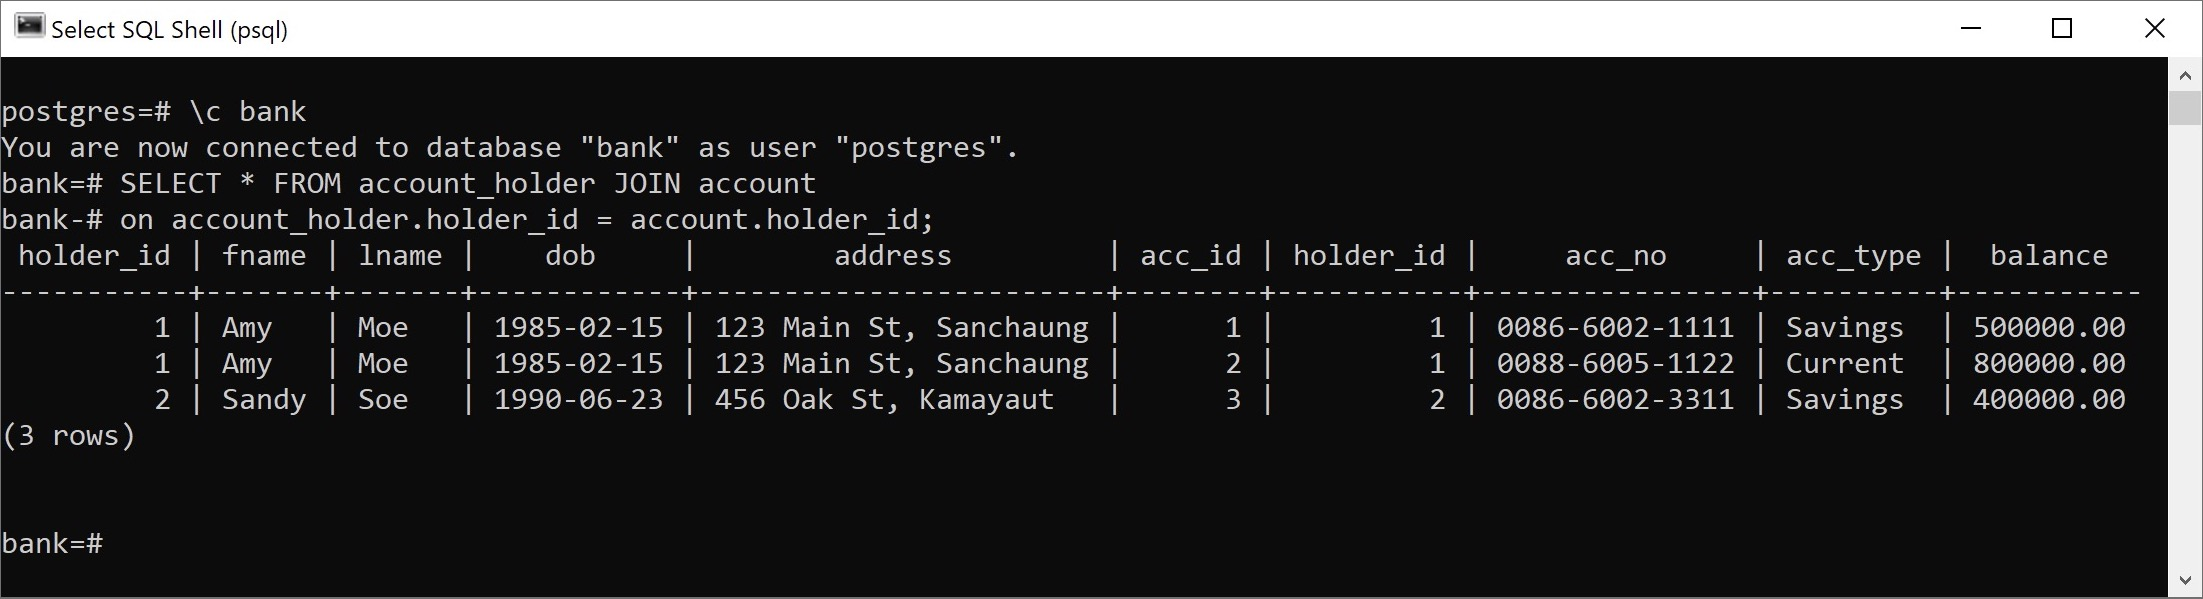
\includegraphics[width=1.13\textwidth, trim={0mm 50mm 0mm 0.5mm},clip]{images/ch12/join.jpg}};
  \drawshadow{image}
\end{tikzpicture}
\caption{table နှစ်ခု join ပြီး select လုပ်ထားတာ} 
\label{fig:join}
\end{figure}
\fCode{account\_holder} \fEn{table} ရဲ့ \fCode{holder\_id} နဲ့  \fCode{account} \fEn{table} ရဲ့ \fCode{holder\_id} တူရင် \fCode{JOIN} က \fEn{record} တွေကို တွဲဆက်ပေးတာ တွေ့ရမှာပါ။ တွဲဆက်ပေးရမဲ့ ကွန်ဒီရှင်ကို \fCode{ON} နောက်မှာ အခုလို ထည့်ပေးထားတယ်
%
\begin{sql}
ON account_holder.holder_id = account.holder_id;
\end{sql}
%
အောက်မှာ နောက်ထပ် ပုံစံတစ်မျိုး ရေးထားတာကို ကြည့်ပါ။ \fCode{account\_holder} \fEn{table} ကို \fCode{t1} ၊ \fCode{account} ကို \fCode{t2} နဲ့ ရည်ညွှန်းပါတယ်။ \fEn{Alias} လုပ်တာလို့ ခေါ်ပါတယ်။
%
\begin{sql}
SELECT 
    t1.*,
    t2.* 
FROM account_holder t1 JOIN account t2
    ON t1.holder_id = t2.holder_id;
\end{sql}
%
\fEn{Table} နှစ်ခုကနေ လိုချင်တဲ့ \fEn{column} ကိုပဲ ရွေးထုတ်လည်း ရတယ်။ ဥပမာ
%
\begin{sql}
SELECT 
    t2.*,
    t1.fname,
    t1.lname
FROM account_holder t1 JOIN account t2
    ON t1.holder_id = t2.holder_id;
\end{sql}
%

\subsection*{Referential Integrity}
\fEn{Relational Model} ဟာ \fEnEmp{referential integrity} ကို မပျက်ယွင်းအောင် အလေးအနက်ထား  ထိန်းသိမ်းပေးပါတယ်။ \fEn{Record} တစ်ခုကို ဖျက်တဲ့အခါ အဲဒီဖျက်လိုက်တဲ့ \fEn{record} ကို အခြား \fEn{table} မှာရှိတဲ့ \fEn{record} တွေက ရည်ညွှန်းထားမယ်ဆိုရင် ပြဿနာရှိတယ်။ ဥပမာ \fCode{account\_holder} \fEn{table} မှာ အကောင့်ပိုင်ရှင် အေမီ့ \fEn{record} ကို ဖျက်လိုက်တယ် ဆိုပါစို့။ ဒီလိုဆိုရင် \fCode{account} \fEn{table} ထဲက \fCode{holer\_id} $1$ နဲ့ အကောင့်နှစ်ခု ရည်ညွှန်းထားတဲ့ အကောင့်ပိုင်ရှင် \fEn{record} ရှိမှာ မဟုတ်တော့ဘူး။ ဒါဟာ \fEn{referential integrity} ကို ချိုးဖောက်တာ ဖြစ်တဲ့အတွက် \fEn{Relational Model} က အဲဒီလို ဖျက်ခွင့်ပေးမှာ မဟုတ်ပါဘူး။ \fEn{Record} တစ်ခုကို အခြား \fEn{record} တွေက \fEn{reference} လုပ်ထားတာ ရှိနေသ၍ \fEn{Relational Model} က အဲ့ဒီ \fEn{record} ပေးမဖျက်ဘူး။ အခုလို စမ်းပြီး ဖျက်ကြည့်ပါ။ 
%
\begin{figure}[tbh!]
\begin{tikzpicture}
  \node[anchor=south west,inner sep=0] (image) at (0,0)
  {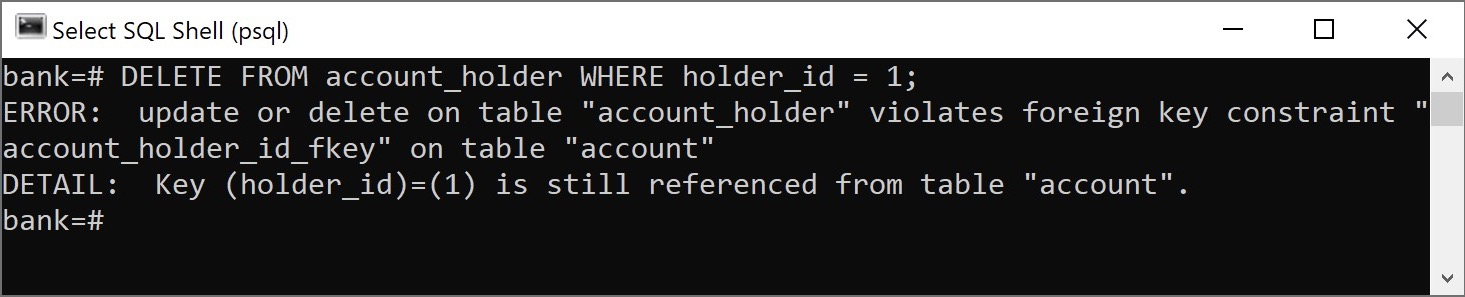
\includegraphics[width=.98\textwidth, trim={0.5mm 0mm 0mm 0.8mm},clip]{images/ch12/ref_integrity.jpg}};
  \drawshadow{image}
\end{tikzpicture}
\caption{referential integrity အရ ပေးမဖျက်တာ} 
\label{fig:ref_integrity}
\end{figure}%
ဖျက်ခွင့်မပေးတာကို တွေ့ရပါလိမ့်မယ်။

\fCode{holer\_id} $1$ နဲ့ \fEn{record} ကို ဖျက်ချင်ရင် ၎င်းကို ရည်ညွှန်းတဲ့ \fEn{record} တွေကို အရင်ဖျက်ရပါမယ်။ ဒါမှမဟုတ် နောက်ထပ်နည်းလမ်းတစ်ခုက \fEn{parent record} ကိုဖျက်ရင် ဆက်စပ်နဲ့တဲ့ \fEn{child record} တွေကိုပါ အလိုအလျောက် ဖျက်အောင် \fCode{ON DELETE CASCADE} \fEn{option} အသုံးပြုတာပါ။ ရည်ညွှန်းတဲ့ \fEn{table/record} ကို \fEn{child table/record} လို့ ယူဆပါ။ ရည်ညွှန်းခြင်း ခံရတဲ့ \fEn{table/record} ကို \fEn{parent table/record} လို့ ယူဆပါ။ \fCode{ON DELETE CASCADE} ကို \fEn{child table} ဆောက်တဲ့အခါ \fCode{holder\_id} \fEn{column} မှာ အခုလို သတ်မှတ်ပေးရမှာပါ။
%
\begin{sql}
CREATE TABLE account (
    acc_id SERIAL PRIMARY KEY,
    holder_id INT REFERENCES account_holder(holder_id) ON DELETE CASCADE,
    ß$\ldots$ß
);
\end{sql}
%

\fEn{Referential integrity} နဲ့ ပါတ်သက်ပြီး နားလည်ထားဖို့ လိုပါတယ်။ ဒါကြောင့် အကျဉ်းချုံး ရှင်းပြထားတာပါ။ \fCode{ON DELETE CASCADE} စမ်းကြည့်မယ်ဆို ဒေတာဘေ့စ် ကိုဖျက်ပြီး \fEn{table} ပြန်ဆောက် (သို့) ဒေတာဘေ့စ် အသစ်တစ်ခု ဆောက်ပြီး စမ်းကြည့်ပါ။ ရှိပြီးသား \fEn{table} ကို \fCode{ON DELETE CASCADE} ဖြစ်အောင် လုပ်လို့ရပေမဲ့ နည်းနည်းပိုရှုပ်ထွေးပါတယ်။

\subsection*{Relationship Between \fSubSecCodeBf{account} and \fSubSecCodeBf{account\_transaction} Tables}
\fEn{Table relationship} နဲ့ \fCode{JOIN} ကို ပိုပြီး သဘောပေါက်အောင် အားဖြည့်တဲ့အနေနဲ့ နောက်ထပ် ဥပမာတစ်ခု ကြည့်ရအောင်။ အကောင့် ငွေသွင်း/ထုတ်စာရင်း \fEn{(account transaction)} \fEn{table} ပါ။
%
\begin{sql}
CREATE TABLE account_transaction (
    txn_id SERIAL PRIMARY KEY,
    -- reference to account table by acc_id
    acc_id INT REFERENCES account(acc_id),
    txn_date TIMESTAMP DEFAULT CURRENT_TIMESTAMP,
    txn_type VARCHAR(20),
    amount NUMERIC(12, 2),
    balance_after NUMERIC(12, 2)
);
\end{sql}
%
ဒီ \fEn{table} မှာ \fCode{acc\_id} \fEn{column} က \fCode{account} \fEn{table} ရဲ့ \fCode{acc\_id} \fEn{column} ကို \fEn{reference} လုပ်ထားတာ ဂရုပြုကြည့်ပါ။ အောက်ပါ ငွေသွင်း/ထုတ် စာရင်း \fEn{(transaction)} ၅ ခု ထည့်ပါ 
%
\begin{sql}
INSERT INTO account_transaction 
    (acc_id, txn_date, txn_type, amount, balance_after)
VALUES 
    (1, '2024-08-01 09:00:00', 'Deposit', 100000.00, 600000.00),
    (1, '2024-08-05 14:30:00', 'Withdrawal', 50000.00, 550000.00),
    (2, '2024-08-02 10:00:00', 'Deposit', 200000.00, 1000000.00),
    (2, '2024-08-03 16:00:00', 'Withdrawal', 300000.00, 700000.00),
    (3, '2024-08-04 11:00:00', 'Deposit', 50000.00, 450000.00);
\end{sql}
%
\fEn{Table} နှစ်ခုကို \fCode{acc\_id} နဲ့ ဘယ်လို ချိတ်ဆက်ထားလဲ နားလည်ဖို့ အရေးကြီးတယ်။ ပထမ \fEn{transaction} နှစ်ခုနဲ့ သက်ဆိုင်တဲ့ အကောင့် အချက်အလက် အသေးစိတ်ကို သိချင်ရင် \fCode{account} \fEn{table} မှာ \fCode{acc\_id} နံပါတ် $1$ နဲ့ \fEn{record} ကို ကြည့်ရမှာပါ
%
\begin{sql}
SELECT * FROM account WHERE acc_id = 1;
\end{sql}
%
%
\begin{vbtm}
ß\fEnBf{Output:}ß
 acc_id | holder_id |     acc_no     | acc_type |  balance
--------+-----------+----------------+----------+-----------
      1 |         1 | 0086-6002-1111 | Savings  | 500000.00
\end{vbtm}
%
\fCode{account\_transaction} \fEn{table} မှာ \fEn{transaction record} တွေ  \fEn{insert} လုပ်တဲ့အခါမှာလည်း ၎င်းတို့နှင့် သက်ဆိုင်တဲ့ \fCode{acc\_id} ကို မှန်ကန်အောင် သေချာစိစစ်ဖို့ လိုတယ်။ \fEn{Table} နှစ်ခုက အချက်အလက်တွေကို \fCode{JOIN} နဲ့ ချိတ်ဆက် ထုတ်ယူနိုင်တယ်။

%
\begin{sql}
SELECT 
    *
FROM account t1 JOIN account_transaction t2
    ON t1.acc_id = t2.acc_id;
\end{sql}
%
\fEn{Table} နှစ်ခုမကလည်း \fCode{JOIN} လို့ရတယ်။ ဥပမာ 
%
\begin{sql}
SELECT 
    t1.holder_id,
    t1.fname,
    t1.lname,
    t2.acc_no,
    t2.acc_type,
    t3.txn_type,
    t3.amount,
    t3.balance_after
FROM account_holder t1 JOIN account t2
    ON t1.holder_id = t2.holder_id
JOIN account_transaction t3
    ON t2.acc_id = t3.acc_id;
\end{sql}
%

\fEn{Table} သုံးခုကြား \fEn{relationship} ကို နားလည်အောင် နောက်ဆုံးတစ်ခါ အောက်ပါတို့ကို ဆက်စပ်ကြည့်ပါ။ \fEn{Insert} တစ်ခါလုပ်ပြီး \fEn{auto-generated id} နံပါတ်တွေ \fEn{select} လုပ်ကြည့်ပါ။
%
\begin{sql}
INSERT INTO account_holder (fname, lname, dob, address)
VALUES 
('Waiyan', 'Phyo', '1991-07-22', '45 Bawga St, Yankin');
\end{sql}
%
%
\begin{sql}
-- Before insert, make sure Waiyan's holder_id is 3
INSERT INTO account (holder_id, acc_no, acc_type, balance)
VALUES 
(3, '0086-6002-4411', 'Savings', 700000.00);
\end{sql}
%

%
\begin{sql}
-- Before insert, make sure Waiyan's acc_id is 4
INSERT INTO account_transaction 
    (acc_id, txn_date, txn_type, amount, balance_after)
VALUES 
    (4, '2024-08-05 15:45:00', 'Deposit', 200000.00, 900000.00);
\end{sql}
%


\section{SQL ဖန်ရှင်များ}
\fEn{SQL} မှာ \fEn{built-in} ဖန်ရှင်တွေ ပါရှိပါတယ်။ \fCode{to\_char}\fEn{,} \fCode{upper} နဲ့ \fCode{concat} သုံးထားတာ ကြည့်ပါ။ \fEn{Column} ကို \fEn{alias} ပေးလို့ရတယ်။ \fCode{Date\_of\_Birth} နဲ့ \fCode{Full\_Name} က \fEn{alias} တွေ။
%
\begin{sql}
SELECT
    to_char(dob, 'Mon DD YYYY') Date_of_Birth,
    upper(concat(fname, ' ', lname)) Full_Name
FROM account_holder;
\end{sql}
%
%
\begin{vbtm}
ß\fEnBf{Output:}ß
 date_of_birth |  full_name
---------------+-------------
 Feb 15 1985   | AMY MOE
 Jun 23 1990   | SANDY SOE
 Jul 22 1991   | WAIYAN PHYO
(3 rows)
\end{vbtm}
%
%
\begin{flushleft}
\vspace{1em}
\setlength{\extrarowheight}{3pt}
\begin{tabular}[!htb]{*{3}l}
    \toprule[1.5pt]
    \fTblHead{Format Code} & \fTblHead{Format}  \\        
    \midrule
    \fCode{YYYY}     & \fEn{Year (4 digits)} \\
    \fCode{YY}       & \fEn{Year (last 2 digits)} \\
    \fCode{MM}       & \fEn{Month (01-12)} \\
    \fCode{MON}      & \fEn{Abbreviated month name (e.g., AUG)} \\
    \fCode{MONTH}    & \fEn{Full month name (e.g., AUGUST)} \\
    \fCode{DD}       & \fEn{Day of the month (01-31)} \\
    \fCode{HH24}     & \fEn{Hour (24-hour clock, 00-23)} \\
    \fCode{HH12}     & \fEn{Hour (12-hour clock, 01-12)} \\
    \fCode{MI}       & \fEn{Minute (00-59)} \\
    \fCode{SS}       & \fEn{Second (00-59)} \\
    \fCode{AM/PM}    & \fEn{Meridian indicator} \\
    \bottomrule[1.5pt]
\end{tabular}
\label{tbl:psqldtfmt}
\captionof{table}{PostgreSQL Date and Time Format Codes}
\end{flushleft}
%
\fEn{SQL} \fCode{date} (သို့) \fCode{datetime} \fEn{data type} ကနေ လိုချင်တဲ့ \fEn{format} ကို \fCode{to\_char} ဖန်ရှင်နဲ့ ပြောင်းလို့ရတယ်။ \fCode{'Mon DD YYYY'} မှာ \fCode{Mon} က \fEn{month} ကို \fEn{Feb, Jun, Jul} အတိုကောက်ပြဖို့။ \fEn{Format codes} တွေကို ဇယား (\fRefNo{\ref{tbl:psqldtfmt}}) တွင် ကြည့်ပါ။

အောက်ပါအတိုင်း အလွယ်တကူ စမ်းကြည့်လို့ ရပါတယ်။ လက်ရှိအချိန်ကို \fCode{now()} နဲ့ ယူတယ်။ ဒီလို \fEn{format} \fCode{15/08/2024 10:41:36} နဲ့ ထုတ်ပေးမှာပါ။
%
\begin{sql}
SELECT to_char(now(), 'DD/MM/YYYY HH24:MI:SS') formatted_datetime;
\end{sql}
%

အခြား ဖန်ရှင်တွေ အများကြီး ရှိပါသေးတယ်။ ဒီစာအုပ်မှာတော့ ဒီလောက်ပဲ အကျဉ်း ဖော်ပြပေးနိုင်ပါတယ်။ ဘီဂင်နာတွေ ဆက်လက်လေ့လာဖို့ စာအုပ်၊ \fEn{YouTube} နဲ့ \fEn{tutorial} လင့်တချို့ကို ဒီအခန်းအဆုံးမှာ ပေးထားတယ်။ 

%https://www.tutorialspoint.com/postgresql/index.htm
%https://postgrespro.com/community/books/introbook
%https://www.postgresql.org/docs/15/index.html
%https://www.youtube.com/playlist?list=PL7D4X4pSOcCGoKVKDNjeKLRDK4TNRxc1x
%https://pg-sql.com/
%https://www.youtube.com/playlist?list=PLavw5C92dz9Ef4E-1Zi9KfCTXS_IN8gXZ
%https://www.youtube.com/watch?v=NTgejLheGeU&t=12290s

\section{Python နှင့် ဒေတာဘေ့စ် ပရိုဂရမ်းမင်း}
ဆော့ဖ်ဝဲ အပ်ပလီကေးရှင်းတွေဟာ ဒေတာဘေ့စ်နဲ့ ချိတ်ဆက်လုပ်ဆောင် ရလေ့ရှိတယ်။ \fEn{‘End User’} လို့ခေါ်တဲ့ အသုံးပြုသူတွေဟာ အပ်ပလီကေးရှင်း \fEn{User Interface (UI)} ကနေတစ်ဆင့် ဒေတာဘေ့စ်ကို သုံးကြတာပါ။ ပုံမှန်အားဖြင့် \fEn{end user} အများစုဟာ ဒေတာဘေ့စ်ကို တိုက်ရိုက် အသုံးမပြုကြပါဘူး။ ဒါကြောင့် \fEn{end user} တွေလိုအပ်မဲ့ ဒေတာသွင်းတာ၊ ပြန်ရှာ/ဖတ်တာ၊ အပ်ဒိတ်လုပ်တာ၊ ဖျက်တာ စတဲ့ကိစ္စတွေအတွက် အပ်ပလီကေးရှင်းတွေကပဲ ထည့်သွင်းစဉ်းစား တည်ဆောက်ပေးရတာပါ။ 

ကျောင်းသားစာရင်းသွင်း ပရိုဂရမ်တစ်ခုကို စိတ်ကူးကြည့်ပါ။ ကျောင်းသားသစ် ကိုယ်ရေး အချက်အ\allowbreak လက် \fEn{UI} နမူနာကို ပုံ (\fRefNo{\ref{fig:stuform}}) မှာ ပြထားတာ ကြည့်ပါ။ \fEn{Submit} နှိပ်လိုက်ရင် ဖြည့်ထားတဲ့ ကျောင်းသား အချက်အလက်တွေကို ဒေတာဘေ့စ်ထဲ သိမ်းရပါမယ်။ ထိုနည်းတူစွာ ပြန်ရှာတာ၊ ဖျက်တာ၊ \fEn{update} လုပ်တာ ကိုလည်း \fEn{UI} ကနေပဲ လုပ်လို့ရအောင် ပရိုဂရမ်က စီစဉ်ပေးထားရမှာပါ။ 
%
\begin{figure}[tbh!]
\begin{tikzpicture}
  \node[anchor=south west,inner sep=0] (image) at (0,0)
  {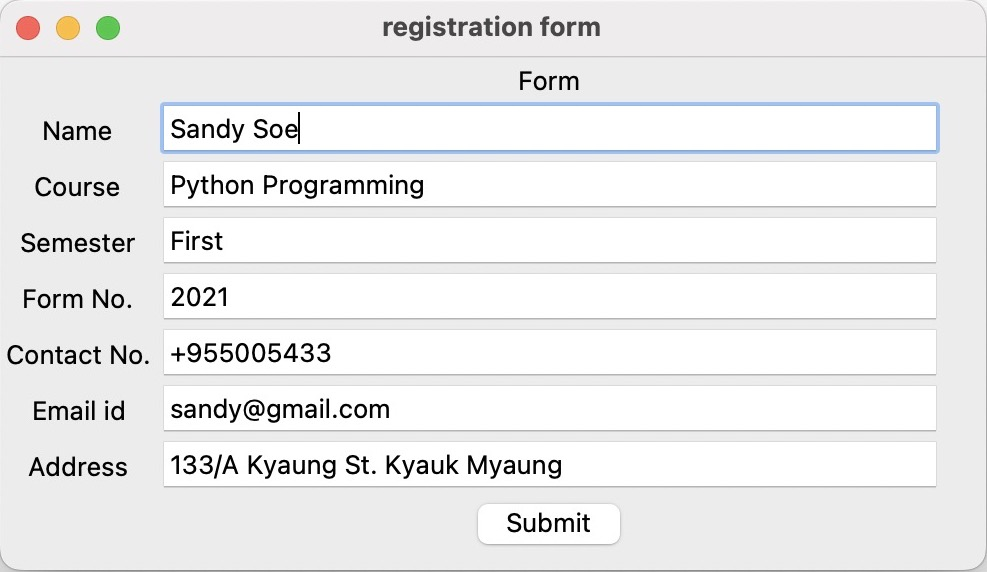
\includegraphics[width=.75\textwidth, trim={0mm 0mm 0mm 0mm},clip]{images/ch12/stuform.jpg}};
  \drawshadow{image}
\end{tikzpicture}
\caption{} 
\label{fig:stuform}
\end{figure}
%

ဒီလို အပ်ပလီကေးရှင်းမျိုးတွေကို ဒေတာဘေ့စ် အပ်ပလီကေးရှင်းလို့ ခေါ်ပါတယ်။ အချက်အလက်တွေ \fEn{create, read, update, and delete} လုပ်တဲ့ အခြေခံလုပ်ဆောင်ချက် လေးခု ပါဝင်တာကြောင့်မို့ \fEn{CRUD} အပ်ပလီကေးရှင်းလို့လည်း ခေါ်ကြတယ်။  

\subsection*{Psycopg ဒေတာဘေ့စ် ဒရိုက်ဗာ}
% Psycopg is the most popular PostgreSQL database adapter for the Python programming language. 
\fEn{Python} နဲ့ \fEn{PostgreSQL} ချိတ်ဆက်လုပ်ဆောင်ဖို့အတွက် \fEn{Psycopg} (ဆိုက်ကော့ပ်ဂျီ) ဟာ လူကြိုက်အများဆုံး ဒေတာဘေ့စ် ဒရိုက်ဗာ ဖြစ်ပါတယ်။ ဒေတာဘေ့စ် ဒရိုက်ဗာဆိုတာ ဒေတာဘေ့စ်နဲ့ \fEn{programming language} ကြား ပေါင်းကူးတံတားအဖြစ် ဆောင်ရွက်ပေးတဲ့ လိုက်ဘရီပါ။ ဒေတာဘေ့စ် အဒပ်တာ \fEn{(adapter)} လို့လည်းခေါ်တယ်။

\fEn{DBMS} နဲ့ \fEn{programming language} အလိုက် သက်ဆိုင်ရာ ဒေတာဘေ့စ် ဒရိုက်ဗာကို ရွေးချယ် အသုံးပြုရမှာပါ။ \fEn{PostgreSQL} အတွက် \fEn{Python} မှာ \fEn{Psycopg 2} နဲ့ \fEn{Psycopg 3} ရှိမယ်။ အခြားဟာတွေလည်း ရှိပါသေးတယ်။ \fEn{MySQL} အတွက် \fEn{MySQL Connector/Python} သုံးကြတယ်။ \fEn{Microsoft SQL} အတွက်ဆိုရင် \fEn{pyodbc} ဒရိုက်ဗာ။ 

\fEn{Psycopg 3} က ဗားရှင်းပိုမြင့်ပေမဲ့ ဒီစာအုပ်မှာ \fEn{Psycopg 2} ကိုပဲ အသုံးပြုပါမယ်။ \fEn{Psycopg 2} သုံးတတ်ရင် \fEn{Psycopg 3} ပြောင်းသုံးလည်း အခက်အခဲ သိပ်မရှိနိုင်ဘူး။ ဘီဂင်နာအတွက် စလေ့လာရတာ ပိုအဆင်ပြေမယ် ယူဆတာကြောင့် \fEn{Psycopg 2} သုံးဖို့ ဆုံးဖြတ်ရတာပါ။ နောက်ပိုင်း အတွေ့အကြုံရှိလာရင် ဗားရှင်းအမြင့်ကို ဆက်လေ့လာလို့ရပါတယ်။ \fEn{Psycopg 2} ကို အောက်ပါအတိုင်း \fCode{pip} ကွန်မန်းနဲ့  အင်စတောလ်လုပ်ပါ။
%
\begin{codetxt}
pip install psycopg2-binary 
\end{codetxt}
%


\subsection*{Connecting to PostgreSQL}
ဒေတာဘေ့စ် အပ်ပလီကေးရှင်းတွေဟာ \fEn{client-server} အပ်ပလီကေးရှင်းတွေလို့ ရှေ့ပိုင်းမှာ ပြောခဲ့တာ မှတ်မိမယ်ထင်ပါတယ်။ အချက်အလက်တွေ အပြန်အလှန် ပေးပို့လုပ်ဆောင်နိုင်ဖို့ \fEn{client} နဲ့ \fEn{server} ကြား ကွန်နက်ရှင် ချိတ်ဆက်ဖို့လိုတယ်။ ဒီလိုချိတ်ဆက်တဲ့အခါ \fEn{TCP/IP (Transmission Control Protocol/Internet Protocol)} ကို အသုံးပြုရပါတယ်။ \fEn{CRUD} အော်ပရေးရှင်း တစ်ခုခု လုပ်မယ်ဆို ပထမဆုံး ကွန်နက်ရှင်အရင် ရှိထားရမှာပါ။ ကွန်နက်ရှင်မရရင် ဒေတာဘေ့စ်နဲ့ ပါတ်သက်တဲ့ အခြားကိစ္စတွေ ဆက်လုပ်လို့ မရနိုင်ဘူး။ 

ပထမ ဥပမာအနေနဲ့ \fEn{Python} ပရိုဂရမ်ကနေ \fEn{PostgreSQL} ဒေတာဘေ့စ် အသစ်တစ်ခု ဘယ်လိုဆောက်ရမလဲ ကြည့်ရအောင်။ 
%
\begin{py}
# File: db_connect.py
import psycopg2

# Connect to the default PostgreSQL database to create 
# the new "students" database
conn = psycopg2.connect(
    dbname="postgres",
    user="postgres",
    password="asdfgh",
    host="localhost",
    port="5432"
)

conn.autocommit = True
cur = conn.cursor()

# Create the "students" database
cur.execute("DROP DATABASE IF EXISTS students")
cur.execute("CREATE DATABASE students")

# Close the initial connection
cur.close()
conn.close()
\end{py}
%

ဒီပရိုဂရမ်ကို တစ်ခုချင်း ခွဲခြမ်းစိတ်ဖြာ ကြည့်ပါမယ်။ \fCode{psycopg2} လိုက်ဘရီ ပထမဆုံး အင်ပို့ လုပ်ထားတယ်။ ပြီးတော့ \fCode{connect} ဖန်ရှင်နဲ့ ကွန်နက်ရှင်ယူတယ်။ \fCode{connect} ဖန်ရှင် ပါရာမီတာတွေက \fEn{psql} နဲ့ ကွန်နက်လုပ်တဲ့အခါ ထည့်ပေးရတာတွေနဲ့ တူတူပါပဲ။
%
\begin{itemize}
    \item \fCode{dbname} (ချိတ်ဆက်မဲ့ ဒေတာဘေ့စ်နံမည်) 
    \item \fCode{user} (ဒေတာဘေ့စ် ချိတ်ဆက်အသုံးပြုမဲ့ \fEn{user}) 
    \item \fCode{password} (ဒေတာဘေ့စ်ကို ချိတ်ဆက်အသုံးပြုမဲ့ \fEn{user} ရဲ့ \fEn{password})
    \item \fCode{host} (ချိတ်ဆက်မဲ့ ဆာဗာရဲ့ \fEn{Host Name/IP Address})
    \item \fCode{port} (\fEn{PostgreSQL port} နံပါတ်)
\end{itemize}
%

\fEn{Connect} လုပ်တာ အောင်မြင်ရင် \fCode{connect} ဖန်ရှင်က \fCode{connection} အော့ဘ်ဂျက်တစ်ခု ပြန်ရပါတယ်။ တကယ်လို့ ပြဿနာ တစ်ခုခုကြောင့် \fEn{connect} လုပ်လို့ မရရင်တော့ ဖြစ်ရတဲ့ အကြောင်းအရင်းပေါ် မူတည်ပြီး \fCode{OperationalError}\fEn{,} \fCode{InternalError} စတဲ့ \fEn{exception} တွေ တက်နိုင်တယ်။ ဒီ \fEn{exception} တွေက \fCode{psycopg2.Error}  ရဲ့ \fEn{subclass} တွေပါ။


%
\begin{py}
conn.autocommit = True
\end{py}
%
ဒါက ဒေတာဘေ့စ် \fEn{auto-commit mode} ကို \fEn{on} လုပ်ပေးဖို့။ ဒေတာဘေ့စ် \fEn{transaction} နဲ့ ဆိုင်တဲ့ \fEn{setting} တစ်ခုဖြစ်ပြီး နောက်ပိုင်းမှာ အသေးစိတ် ရှင်းပြမှာပါ။ \fEn{Psycopg} က သူ့နဂိုအတိုင်းဆိုရင်  \fEn{auto-commit mode} ကို \fEn{off} လုပ်ထားတယ်။ ဒေတာဘေ့စ် အသစ်ဆောက်တဲ့ \fCode{CREATE DATABASE} လို တချို့ \fEn{SQL} စတိတ်မန့်တွေက \fEn{auto commit} ကို \fEn{on} လုပ်ပေးရတယ်လို့ လောလောဆယ် သိထားရင် လုံလောက်ပါပြီ။ \fEn{Auto-commit on} ထားရင် \fEn{SQL} စတိတ်မန့်တွေ \fCode{execute} လုပ်ပြီးရင် \fCode{commit} ဖန်ရှင် ခေါ်ဖို့ မလိုဘူး။ (နောက် ဥပမာမှာ \fCode{commit} ဖန်ရှင် သုံးထားတာ တွေ့ရမှာပါ)။

\fEn{SQL} စတိတ်မန့်တွေ ဒေတာဘေ့စ်ဆီ ပေးပို့လုပ်ဆောင်စေခြင်း၊ ဒေတာဘေ့စ်ဆီက ပြန်ရလာတဲ့ ရလဒ်တွေကို အသုံးပြုခြင်း၊ ဒေတာဘေ့စ် \fEn{transaction} စီမံခြင်း စတဲ့ ကိစ္စတွေအတွက် \fEn{cursor} က အဓိကကျတယ်။ \fEn{Cursor} အော့ဘ်ဂျက်ကို \fEn{connection} ကနေ တစ်ဆင့် အခုလို ယူရပါတယ်
%
\begin{py}
cur = conn.cursor()
\end{py}
%

ချိတ်ဆက်ထားတဲ့ ဒေတာဘေ့စ်ဆီကို \fEn{SQL} စတိတ်မန့်တွေ ပေးပို့ လုပ်ဆောင်ခိုင်းဖို့ \fCode{execute} ဖန်ရှင် အသုံးပြုတယ်။  
%
\begin{py}
cur.execute("DROP DATABASE IF EXISTS students")
cur.execute("CREATE DATABASE students")
\end{py}
%
 ပထမ တစ်ကြောင်းက \fCode{students} ဒေတာဘေ့စ် ရှိပြီးသားဆိုရင် ဖျက်ပစ်မှာပါ။ ပြီးတော့မှ ဒုတိယ တစ်ကြောင်းမှာ ဒေတာဘေ့စ် အသစ်ဆောက်ပါတယ်။ ရှိပြီးသားဆိုရင် ဖျက်ပြီး အသစ်ပြန်ဆောက်တဲ့ သဘောပါ။ \fEn{psql} နဲ့ဆိုရင် \fEn{SQL} စတိတ်မန့်အဆုံးမှာ \fCode{;} ထည့်ပြီး \fEn{run} ရမှာ ဖြစ်ပေမဲ့ \fEn{Psycopg} မှာတော့ ထည့်စရာ မလိုဘူး။ ထည့်ပေးလည်း ပြဿနာတော့ မရှိဘူး။


\fEn{Cursor} နဲ့ \fEn{connection} ကို အသုံးပြုပြီးသွားရင် ပိတ်ပေးရပါမယ်။ \fEn{Exception handle} လုပ်မယ်ဆိုရင် \fCode{finally} ထဲမှာ ပိတ်သင့်တယ်။ ဒီဥပမာမှာတော့ ဒီတိုင်းပဲ ပိတ်ထားပါတယ်။
%
\begin{py}
cur.close()
conn.close()
\end{py}
%
ဒီပရိုဂရမ် \fEn{run} ပြီး \fEn{error} လည်း မတက်ဘူးဆိုရင် \fEn{students} ဒေတာဘေ့စ် ဆောက်ပြီးသွားမှာပါ။ \fEn{psql} ကနေ \mintinline{text}|\l| ကွန်မန်းနဲ့ စစ်ကြည့်နိုင်ပါတယ်။









ဒေတာဘေ့စ်ထဲမှာ \fEn{table} တွေ ဆောက်ပါမယ်။ လက်ရှိအသုံးပြုမဲ့ ဒေတာဘေ့စ်နဲ့ \fEn{connection} အရင်ယူရမယ်။ \fEn{students} ဒေတာဘေ့စ်မှာ  \fEn{table} ဆောက်မှာ။ ဒီတော့ ချိတ်ဆက်မဲ့ \fCode{dbname} က \fCode{students} ဖြစ်တယ်။ ကျန်တာတွေက ရှေ့ကနဲ့ တူတူပဲ။
%
\begin{py}
# File: db_create_student_tbl.py
import psycopg2

# Now, connect to the "students" database to create the "student" table
conn = psycopg2.connect(
    dbname="students",
    user="postgres",
    password="asdfgh",
    host="localhost",
    port="5432"
)
conn.autocommit = False
cur = conn.cursor()

# Create the "student" table
cur.execute("""
    CREATE TABLE student (
        id SERIAL PRIMARY KEY,
        name VARCHAR(100),
        age INT,
        grade VARCHAR(2)
    )
""")

# Commit changes and close the connection
conn.commit()
cur.close()
conn.close()
\end{py}
%
ကွန်နက်ရှင် ရပြီး နောက်မှာ
%
\begin{py}
conn.autocommit = False
\end{py}
%
နဲ့ \fEn{auto-commit mode} ကို \fEn{off} လုပ်တယ်။ \fEn{Psycopg} \fEn{default} က \fEn{auto-commit off} ဖြစ်တဲ့အတွက် ဒါမပါရင်လည်း \fEn{off} ဖြစ်နေမှာပါ။ ဒါဆို ဘာလို့ တကူးတက ထည့်ထားလည်းဆိုတော့ ကုဒ်ကို ဖတ်တဲ့အခါ \fEn{auto-commit off} ထားတယ်ဆိုတာ သိသာစေချင်တာရော ဒရိုက်ဗာရဲ့ \fEn{default} က \fEn{on/off} ဘာလဲ မသေချာမှာ စိုးလို့ပါ။  

\fCode{CREATE TABLE} စတိတ်မန့်က  \fEn{auto-commit mode} \fEn{on} ဖြစ်ဖြစ်၊ \fEn{off} ဖြစ်ဖြစ် \fEn{run} လို့ရတယ်။ အခု \fEn{off} လုပ်ထားတာက ရှေကဥပမာမှာ \fEn{on} လုပ်ထားတာနဲ့ ကွာခြားချက်တချို့ကို သိအောင်လို့ပါ။ အခြားထူးခြားတဲ့ အကြောင်းအရင်း မရှိပါဘူး။ နောက်ပိုင်း \fEn{database transaction} အပိုင်းမှာ \fEn{off} လုပ်ကို လုပ်ရတဲ့ အကြောင်းအရင်းကို ရှင်းပြပါမယ်။


\fEn{Auto-commit} \fEn{off} ထားရင် \fEn{SQL} စတိတ်မန့် \fEn{execute} လုပ်ပြီး \fEn{commit} လုပ်ပေးဖို့ လိုတယ်။ ဒီအတွက်
%
\begin{py}
conn.commit()
\end{py}
%
လုပ်ရပါမယ်။ \fCode{commit} မလုပ်မိရင် \fEn{execute} လုပ်ထားတဲ့ \fEn{SQL} က သက်ရောက်မှု ရှိမှာမဟုတ်ပါဘူး။ ဆိုလိုတာက \fEn{student table} ဆောက်တဲ့ကိစ္စက အတည်ဖြစ်မသွားဘူး (\fEn{rollback} ဖြစ်သွားတယ်လို့ ခေါ်တယ်)။ \fEn{Commit} နဲ့ \fEn{rollback} အကြောင်း \fEn{transaction} အပိုင်းမှာ ရှင်းပြပါမယ်။

အကယ်၍ \fEn{Auto-commit} \fEn{on} ထားရင်တော့ ကိုယ်တိုင် \fCode{conn.commit()} လုပ်မပေးရဘူး၊ ဒေတာဘေ့စ်က \fEn{SQL} ကွန်မန်း တစ်ခု \fEn{execute} လုပ်ပြီးတိုင်း အလိုအလျောက် \fEn{commit} လုပ်ပေးမှာပါ။ \fEn{Off} ထားရင် \fEn{commit} လုပ်ပေးရမယ်၊ \fEn{on} ဆိုရင် မလုပ်ပေးရဘူးလို့ မှတ်နိုင်ပါတယ်။


\section{Parameterized SQL}
\fEn{SQL} စတိတ်မန့်တွေမှာ ပါရာမီတာ ထည့်လို့ရအောင် ဒေတာဘေ့စ် ဒရိုက်ဗာတွေက ထောက်ပံပေးထားပါတယ်။ ပါရာမီတာပါတဲ့ \fEn{SQL} ကို \fEnEmp{Parameterized SQL} လို့ခေါ်တယ်။ ပုံမှန် ရိုးရိုး \fEn{SQL} နဲ့ \fEn{parameterized SQL} အသုံးပြုပုံ နှစ်ခုယှဉ်ကြည့်ပါ
%
\begin{py}
# normal SQL, no parameter
cur.execute("SELECT * FROM student WHERE age = 19 AND grade = 'A'")
\end{py}
%
%
\begin{py}
# File: db_parameterized_sql.py
# parameterized SQL
age = int(input("Age: "))
grade = input("Grade: ")
cur.execute("SELECT * FROM student WHERE age = %s AND grade = %s",
            (age, grade))
\end{py}
%
\mintinline{text}|%s| က ပါရာမီတာ၊ ပါရာမီတာတွေနေရာ ရှိရမဲ့ တန်ဖိုးအသီးသီးကို \fEn{tuple} နဲ့ ထည့်ပေးရပါမယ်။ \fCode{execute} လုပ်တဲ့အခါ ပါရာမီတာတစ်ခုစီကို သက်ဆိုင်ရာတန်ဖိုး အစားထိုးပေးမှာပါ။ \fEn{Tuple} ဟာ \fEn{list} နဲ့ဆင်တူတဲ့ စထရက်ချာ တစ်မျိုးပါပဲ။ ကွာခြားချက် တချို့ကတော့ \fEn{list} ကို \fCode{[]} သုံးတယ်၊ \fEn{tuple} အတွက် \fCode{()} သုံးတယ်။ \fEn{Tuple} က \fEn{immutable} ဖြစ်ပြီး \fEn{item} တစ်ခုပဲဆိုရင် ကော်မာထည့်ပေးရပါမယ်။ $val_1$ တစ်ခုပဲဆို \mintinline[escapeinside=ßß]{text}|(ß$val_1$ß,)| လို့ ရေးရမှာပါ။ \fEn{Parameterized SQL} မှာ ပါရာမီတာ တစ်ခုတည်းဆိုရင် ဒီအချက်ကို သတိပြုဖို့ လိုပါတယ်။ အောက်မှာ \fCode{(stu\_id,)} ဖြစ်ရပါမယ်။ ကော်မာ မထည့်ဘဲ \fCode{(stu\_id)} လို့ ရေးမိရင် အယ်ရာတက်မှာပါ။
%
\begin{py}
stu_id = int(input("ID: "))
cur.execute("SELECT * FROM student WHERE id = %s", (stu_id,))
\end{py}
%

\fEn{Parameterized SQL} နဲ့ \fEn{insert} ဘယ်လိုလုပ်ထားလဲ အောက်မှာ လေ့လာကြည့်ပါ။ \fCode{students} \fEn{list} ထဲမှာ ကျောင်းသားတစ်ယောက်ချင်းအတွက် \fEn{tuple} တွေ ထည့်ထားပြီး \fCode{for} \fEn{loop} နဲ့ တစ်ခုချင်း \fEn{insert} လုပ်သွားတာကို ဂရုစိုက် နားလည်အောင် ကြည့်ပါ။
%
\begin{py}
# File: db_insert1.py
import psycopg2

conn = psycopg2.connect(dbname="students", user="postgres",
                        password="asdfgh", host="localhost", port="5432")
conn.autocommit = False
cur = conn.cursor()

# Insert records into the student table one at a time
students = [
    ('Amy', 20, 'A'),
    ('Sandy', 22, 'B'),
    ('Kathy', 21, 'C')
]

for student in students:
    cur.execute("""
        INSERT INTO student (name, age, grade)
        VALUES (%s, %s, %s)
    """, student)

conn.commit()
cur.close()
conn.close()
\end{py}
%


ရှေ့က ဥပမာဟာ အောက်ပါ \fEn{insert} စတိတ်မန့် သုံးခုကို တစ်ခုပြီးတစ်ခု ဒေတာဘေ့စ်ဆီ ပေးပို့ လုပ်ဆောင်စေမှာပါ။ 

%
\begin{sql}
INSERT INTO student (name, age, grade) VALUES ('Amy', 20, 'A');
INSERT INTO student (name, age, grade) VALUES ('Sandy', 22, 'B');
INSERT INTO student (name, age, grade) VALUES ('Kathy', 21, 'C');
\end{sql}
%

\fEn{Insert} သုံးခုလုံး တစ်ခါတည်းနဲ့ ပေးပို့ လုပ်ဆောင်စေချင်ရင် \fCode{executemany} ကို သုံးပါတယ်။ \fEn{Tuple array} တစ်ခု ထည့်ပေးရပါမယ်။ \fEn{Array} ထဲက \fEn{tuple} တစ်ခုချင်းအတွက် \fEn{SQL} စတိတ်မန့် တစ်ခုစီ ထုတ်ပေးပြီး အသုတ်လိုက် ဒေတာဘေ့စ်ဆီ ပို့ပေးပါတယ်။
%
\begin{py}
# File: db_insert2.py
students = [
    ('Amy', 20, 'A'),
    ('Sandy', 22, 'B'),
    ('Kathy', 21, 'C')
]

cur.executemany("""
    INSERT INTO student (name, age, grade)
    VALUES (%s, %s, %s)
""", students)
\end{py}
%
စောစောကဥပမာနဲ့ ရလဒ်အားဖြင့်တော့ တူတူပါပဲ။ တစ်ကြောင်းချင်း ပို့တာနဲ့  သုံးကြောင်းလုံး အသုတ်လိုက် တစ်ခါတည်း ပို့တာပဲ ကွာပါတယ်။ အသုတ်လိုက် ပို့တာက နက်ဝပ်အသွားအပြန် \fEn{(network round-trip)} လုပ်ရတာ မများတဲ့အတွက် \fEn{record} တွေ အများကြီး \fEn{insert} လုပ်တဲ့အခါ သိသိသာသာ ပိုပြီးတော့မြန်မှာပါ။ တစ်ကြောင်းချင်း ပို့တာက တစ်ခါပို့တိုင်း နက်ဝပ်အသွားအပြန် ရှိတဲ့အတွက် ပိုကြာမယ်။ နှစ်မျိုးလုံး သူ့နေရာနဲ့သူ ချင့်ချိန်အသုံးပြုရမှာပါ။ ဒါနဲ့ပါတ်သက်လို့ အခုဆက်လက် ဆွေးနွေးမှာ မဟုတ်ပေမဲ့ ဘယ်လိုအခြေအနေမျိုးမှာ ဘယ်ဟာသုံးသင့်လဲ ဆုံးဖြတ်တတ်အောင် ဆက်လက်လေ့လာဖို့ လိုပါလိမ့်မယ်။ 

\section{\fSecCodeBf{fetch}-ing and Using Results}
\fEn{Select} စတိတ်မန့်ရဲ့ ရလဒ် \fEn{record} တွေကို \fCode{fetchall}\fEn{,} \fCode{fetchmany}\fEn{,} \fCode{fetchone} ဖန်ရှင်တွေနဲ့ ရယူအသုံးပြုနိုင်ပါတယ်။ 

\fCode{fetchall} က \fEn{record} အကုန်လုံးကို တစ်ခါတည်းနဲ့ ရယူပေးမှာပါ။ \fEn{Select} လုပ်တဲ့ \fEn{record} အရေအတွက် များလွန်းရင် ဒေတာဘေ့စ်ကနေ \fEn{Python} ပရိုဂရမ်ဘက်ကို ဒေတာအားလုံး လွှဲပြောင်းရောက်ရှိချိန် ကြာနိုင်တဲ့အပြင် ရောက်ရှိလာတဲ့ \fEn{record} တွေအတွက် ကွန်ပျူတာ မမ်မိုရီသုံးရတာကလည်း ပမာဏ များနိုင်ပါတယ်။ \fCode{fetchall} သုံးမယ်ဆိုရင် \fEn{record} အရေအတွက်ကို ထည့်စဉ်းစားဖို့ လိုပါမယ်။
%
\begin{py}
# File: db_select_and_fetch.py
cur.execute("SELECT * FROM student")

rows = cur.fetchall()
for row in rows:
    print(row)
\end{py}
%

\fCode{fetchone} ကိုတော့ \fEn{record} တစ်ခုပဲ ပြန်ရမှာ သေချာတဲ့ အခြေအနေမျိုးမှာ သုံးပါတယ်။ ဥပမာ \fEn{primary key} နဲ့ \fEn{select} လုပ်တဲ့အခါ \fEn{record} တစ်ခုထက် ပိုမရနိုင်ဘူး။
%
\begin{py}
# File: db_select_and_fetch.py
cur.execute("SELECT * FROM student WHERE id = 1")
row = cur.fetchone()
print(row)
\end{py}
% 

\fCode{fetchmany} ကတော့ လိုသလောက် \fEn{record} အရေအတွက်ကိုပဲ ရယူဖို့အတွက်ပါ။ \fEn{Record} အခု ၁၀၀ ရှိတာကို တစ်ခေါက်ကို ၂၀ နဲ့ ၅ ခါ ခွဲပြချင်တဲ့ အခါမျိုးမှာ သုံးနိုင်ပါတယ်။ 
%
\begin{py}
rows = cur.fetchmany(20)
\end{py}
%

\subsection*{Pagination}
\fEn{Record} တွေ အများကြီး တစ်ခါတည်းနဲ့ ပြမဲ့အစား နည်းနည်းချင်း ခွဲပြီး ပြပေးတဲ့နည်းကို အပ်ပလီကေးရှင်းတွေမှာ အသုံးများတာ တွေ့ရပါတယ်။ \fEn{Pagination} လို့ ခေါ်ပါတယ်။ \fEn{Page} တစ်ခုမှာ သတ်မှတ်ထားတဲ့ \fEn{record} အရေအတွက်ကို ပြပေးပြီး \fEn{user} က နောက် \fEn{page} တစ်ခုချင်း ဆက်ကြည့်လို့ရအောင် စီစဉ်ပေးထားတာပါ။ အောက်ပါ ဥပမာမှာ \fCode{fetchmany} သုံးထားတာ လေ့လာကြည့်ပါ။

%
\begin{py}
# File: db_pagination1.py
# Function to fetch a page of student records using fetchmany
def fetch_page(page_size):
    # Fetch rows in batches using fetchmany
    rows = cur.fetchmany(page_size)
    return rows

cur.execute("SELECT * FROM student ORDER BY id")

page_size = 2    # Number of records per page
page_number = 1  # Start with page 1

while True:
    students = fetch_page(page_size)
    
    if not students:
        break  # No more records, exit loop
    
    print(f"Page {page_number}:", students)
    page_number += 1
\end{py}
%

\fCode{fetchmany} နဲ့ နည်းလမ်းအပြင် \fEn{SQL language} ရဲ့ \fCode{LIMIT} နဲ့ \fCode{OFFSET} အသုံးပြုပြီး \fEn{pagination} လုပ်နိုင်ပါတယ်။ 
%
\begin{py}
# File: db_pagination2.py
# Function to fetch a page of student records
def fetch_page(page_size, page_number):
    offset = (page_number - 1) * page_size

    # SQL query with LIMIT and OFFSET for pagination
    select_query = """
        SELECT * FROM student
        ORDER BY id
        LIMIT %s OFFSET %s
    """

    cur.execute(select_query, (page_size, offset))
    rows = cur.fetchall()

    return rows
\end{py}
% 
\fCode{OFFSET} နဲ့ \fCode{LIMIT} ဟာ “\fEn{page} နံပါတ်” နဲ့ “တစ် \fEn{page} မှာ ပါရှိရမဲ့ \fEn{record} အရေအတွက်” ကို ကိုယ်စားပြုတာလို့ အကြမ်းဖျဉ်း ပြောလို့ရပါတယ်။ ဒီနည်းက \fEn{record} အရမ်းများပြီး \fEn{page} အရေအတွက်များတယ်၊ \fEn{page} တစ်ခုချင်း အစဉ်အတိုင်းမဟုတ်ဘဲ ဟိုကျော်ဒီကျော် ကြည့်လို့ရအောင် လုပ်ဖို့လိုတဲ့ အခြေအနေမျိုးမှာ ပိုပြီးအဆင်ပြေနိုင်ပါတယ်။ ပရိုဂရမ်ကုဒ် အပြည့်အစုံကို သက်ဆိုင်ရာ ဖိုင်မှာ ကြည့်နိုင်ပါတယ်။

\subsection*{\fSubSecCodeBf{rowcount} Attribute}
\fEn{Insert, update, delete} လုပ်တာဆိုရင်တော့ \fEn{insert, update, delete} လုပ်လိုက်တဲ့ \fEn{record} အရေအတွက်ကို \fCode{rowcount} \fEn{attribute} နဲ့ သိနိုင်ပါတယ်။
%
\begin{py}
# File: db_update_and_rowcount.py
cur.execute("""
    UPDATE student
    SET grade = %s
    WHERE name = %s
""", ('A+', 'Amy'))
print(cur.rowcount)
\end{py}
%

\section{Python နဲ့ SQL အကြား ဒေတာတိုက်ပ် ပြောင်းလဲခြင်း}
ဒေတာဖော်ပြပုံ မတူကွဲပြားချက်တွေကြောင့် \fEn{Python} နဲ့ \fEn{SQL} \fEn{language} နှစ်ခုကြား ဒေတာအမျိုးအစား လိုက်လျောညီထွေဖြစ်အောင် ပြောင်းလဲမှုတွေ အပြန်အလှန် လုပ်ဆောင်ဖို့ လိုအပ်ပါတယ်။ \fEn{SQL} ပါရာမီတာနေရာမှာ \fEn{Python} ဒေတာတန်ဖိုး အစားထိုးတဲ့အခါ ဒေတာတိုက်ပ် ပြောင်းလဲခြင်းကို \fEn{Psycopg} က လုပ်ဆောင်ပေးပါတယ်။ %ဒေတာဘေ့စ်ကနေ ပြန်ရလာတဲ့ ရလဒ်တွေကို သင့်တော်တဲ့ \fEn{Python} ဒေတာတိုက်ပ်အဖြစ် ပြောင်းလဲပေးခြင်း တို့ကို \fEn{Psycopg} က လုပ်ဆောင်ပေးပါတယ်။ 
%
\begin{py}
# File: db_datatype_conv.py
# select account transactions between two dates
cur.execute("""
    SELECT * FROM account_transaction 
        WHERE txn_date BETWEEN %s AND %s
""", (datetime(2024, 8, 1), datetime(2024, 8, 31)))
rows = cur.fetchall()
\end{py}
% 
\fEn{Python} \fCode{datetime} ကို သင့်တော်တဲ့ \fEn{SQL} ဒေတာအဖြစ် ပြောင်းလဲပေးဖို့ လိုမယ်ဆိုတာ မြင်နိုင်ပါတယ်။ ဒေတာဘေ့စ်ဆီ ပေးပို့မဲ့ \fEn{SQL} ကို အခုလို \fCode{mogrify} ဖန်ရှင်နဲ့ ထုတ်ကြည့်လို့ ရတယ်
%
\begin{py}
sql_str = cur.mogrify("""
    SELECT * FROM account_transaction 
        WHERE txn_date BETWEEN %s AND %s
""", (datetime(2024, 8, 1), datetime(2024, 8, 31)))
print(sql_str.decode('utf-8'))
\end{py}
%
ဒီလို ပြောင်းပေးထားတာ တွေ့ရမှာပါ 
%
\begin{codetxt}
SELECT * FROM account_transaction 
    WHERE txn_date BETWEEN '2024-08-01T00:00:00'::timestamp 
        AND '2024-08-31T00:00:00'::timestamp
\end{codetxt}
%
ဒီတိုင်း စမ်းကြည့်ပါ  
%
\begin{py}
print(cur.mogrify("SELECT %s, %s, %s;", (None, True, False))
         .decode('utf-8'))
# ß\fEn{Output:}ß 'SELECT NULL, true, false;'
print(cur.mogrify("SELECT %s, %s, %s, %s;",
                  (10, 25 ** 25, 10.0, Decimal("10.00"))).decode('utf-8'))
# ß\fEn{Output:}ß 'SELECT 10, 88817841970012523233890533447265625, 10.0, 10.00;'
\end{py}
%
\fCode{None} ကို \fCode{NULL} ပြောင်းပေးပါတယ်။ \fCode{bool}\fEn{,} \fCode{int}\fEn{,} \fCode{long}\fEn{,} \fCode{Decimal} စတာတွေကိုလည်း သင့်တော်တဲ့ \fEn{SQL} တိုက်ပ်အဖြစ် ပြောင်းပေးတယ်။ 

\fEn{Select} လုပ်တဲ့ ရလဒ်ဒေတာတွေကိုလည်း သင့်တော်တဲ့ \fEn{Python} ဒေတာတိုက်ပ် ပြောင်းပေးမှာပါ။ \fEn{Select} လုပ်ရင် \fEn{row} တွေကို \fEn{list} တစ်ခုအနေနဲ့ ရတယ်။ အဲဒီ \fEn{list} ထဲမှာ \fEn{row} တစ်ခုကို \fEn{tuple} တစ်ခုနဲ့ ဖော်ပြတယ်။ \fEn{Row} ကို \fEn{tuple} အနေနဲ့ ဖော်ပြတဲ့အခါ \fEn{column} တန်ဖိုး တစ်ခုချင်းကို \fEn{SQL} ဒေတာ\\တိုက်ပ် အပေါ်မူတည်ပြီး သက်ဆိုင်ရာ \fEn{Python} ဒေတာတိုက်ပ် ပြောင်းပေးပါတယ်။ \fEn{Python} နဲ့ \fEn{SQL} ဒေတာတိုက်ပ် တစ်ခုချင်းအတွက် လိုက်လျောညီထွေဖြစ်အောင် အပြန်အလှန်တွဲဖက်ပေးထားပုံကို \fEn{Psycopg documentation} စာမျက်နှာမှာ အသေးစိတ် ဖော်ပြထားပါတယ် 

\begin{vbtm}
https://www.psycopg.org/docs/usage.html#python-types-adaptation
\end{vbtm}

\section{Dynamic SQL}
ပရိုဂရမ်ကုဒ်ထဲမှာ ပုံသေရေးထားတာ မဟုတ်ဘဲ ပရိုဂရမ် \fEn{run} တဲ့ အချိန်ကျမှ လိုသလို တည်ဆောက်ယူတဲ့ \fEn{SQL} ကို \fEn{Dynamic SQL} လို့ ခေါ်ပါတယ်။ \fEn{Table} နံမည် ထည့်ပေးလိုက်၊ အဲ့ဒီ \fEn{table} ထဲက \fEn{record} တွေကို ထုတ်ပြရမယ်ဆိုပါစို့။ \fEn{Select} စတိတ်မန့်မှာ \fEn{table} နံမည်က ပုံသေဖြစ်လို့ မရတော့ဘူး။ ပထမဆုံး စဉ်းစားမိတာက \fEn{SQL} ကို \fEn{string} နှစ်ခုဆက်ပြီး ထုတ်မယ်ပေါ့။
%
\begin{py}
# Never do like this!!!
tbl_name = input("Enter table name: ")
select_tbl_sql = "SELECT * FROM " + tbl_name 
\end{py}
%
ဒါဟာ လူပြိန်းနည်းနဲ့ \fEn{dynamic SQL} ထုတ်တဲ့ အရိုးရှင်းဆုံး ဥပမာတစ်ခုပဲ။ ဒီနည်းနဲ့ ရတယ်ဆိုပေမဲ့ ရှားရှားပါးပါး ကြုံရခဲတဲ့ ချွင်းချက်အခြေအနေ တချို့ကလွဲလို့ \fEn{string} ဆက်ပြီး \fEn{SQL} ထုတ်တာက လုံးဝကို မလုပ်သင့်တဲ့ အရာပါ။ ဒါတင် မဟုတ်သေးဘူး။ \fEn{f-strings}\fEn{,} \fCode{str.format()}\fEn{,} \fEn{template string}\fEn{,} ပုံစံဟောင်း \mintinline{text}|%| အော်ပရိတ်တာ စတာတွေကိုလည်း \fEn{dynamic SQL} ထုတ်ဖို့ မသုံးသင့်ဘူး။ (\fEn{Python} မှာ \fEnEmp{string interpolation} ပုံစံအမျိုးမျိုးရှိတယ်၊ \fEn{f-strings} ကို စာမျက်နှာ \fRefNo{\pageref{ch07:f-string}} အခန်း \fRefNo{\ref{ch:ch07ctlstmt}} မှာ ဖော်ပြခဲ့ဖူးတယ်၊ \fEn{Python string interpolation} အကြောင်း \fCode{https://tinyurl.com/y4jju285} မှာ ပြည့်ပြည့်စုံစုံ ရှင်းပြထားတာ တွေ့နိုင်တယ်)။ ဘာကြောင့် မသုံးသင့်တာလဲ အကြောင်းအရင်းကို ဒီအခန်း နောက်ဆုံးပိုင်းမှာ အားနည်းချက်/ပြဿနာတွေကို ဖော်ပြထားတာ ဖတ်ပြီးရင် နားလည်သွားပါလိမ့်မယ်။ 


\fEn{Dynamic SQL} အတွက် \fEn{Psycopg} မှာ \fEn{sql} မော်ဒျူး ရှိပါတယ်။ \fEn{String interpolation} နဲ့ \fEn{SQL} ထုတ်ရင် ဖြစ်နိုင်တဲ့ ပြဿနာတွေကို ဖြေရှင်းပေးထားတယ်။ \fEn{Table} နံမည် \fEn{dynamic SQL} ကို အခုလို ရေးရမယ်။
%\fEn{SQL string} ထဲမှာ \fEn{table, column} စတဲ့ \fEn{identifier} တွေကို ပါရာမီတာအနေနဲ့ ထားမယ်ဆိုရင် \mintinline{text}|{}| ကို သုံးရပါမယ်။ \fEn{Select} စတိတ်မန့်မှာ \fEn{table} နံမည် ပုံသေမထားဘဲ ပြောင်းလို့ရချင်တယ် ဆိုပါစို့။ အခုလို လုပ်ရမှာပါ
%
\begin{py}
# File: db_dynamic_sql1.py   
# reqire sql module
from psycopg2 import sql

tbl_name = input("Enter table name: ")
query = sql.SQL("SELECT * FROM {}").format(sql.Identifier(tbl_name))
cur.execute(query)
\end{py}
%
\fEn{SQL string} အစိတ်အပိုင်းတစ်ခုကို ကိုယ်စားပြုဖော်ပြဖို့အတွက် \fCode{sql.SQL} အော့ဘ်ဂျက် သုံးရပါတယ်။ ၎င်းအော့ဘ်ဂျက် ကိုယ်စားပြုတဲ့ \fEn{SQL} အစိတ်အပိုင်းထဲမှာ \mintinline{text}|{}| ကို ဖြည့်ပေးရမဲ့ နေရာအဖြစ် ယာယီ သတ်မှတ်ပေးနိုင်တယ်။ အဲဒီနေရာကို ဖြည့်ပေးဖို့ \fCode{format} မက်သဒ်ကို သုံးရပါမယ်။ အပေါ်က \fCode{SELECT} \fEn{SQL} မှာ \mintinline{text}|{}| ကို \fEn{table} နေရာမှာ ပထမ ထည့်ထားတယ်။ ပြီးတော့မှ \fCode{format} မက်သဒ်ခေါ်ပြီး အဲ့ဒီနေရာမှာ \fCode{tbl\_name} ဖြည့်တယ်။ \mintinline{text}|{}| နေရာမှာ \fEn{string} တိုက်ရိုက် အစားမထိုးဘဲ \fCode{sql.Identifier} အော့ဘ်ဂျက် ပြောင်းပေးဖို့တော့ လိုတယ်။

% ဒီအော့ဘ်ဂျက် ကိုယ်စားပြုတာက စတိတ်မန့် တစ်ကြောင်းလုံး အပြည့်အစုံ ဖြစ်နိုင်သလို \fCode{FROM}\fEn{,} \fCode{WHERE}\fEn{,} \fCode{ORDER BY} စတဲ့ \fEn{SQL} အစိတ်အပိုင်း တစ်ခုခုလည်း ဖြစ်လို့လည်းရတယ်။ 
% အဲဒီနေရာမှာ \fCode{format} မက်သဒ်နဲ့ \fEn{table/column} ရဲ့ နံမည်ကို အစားထိုး ဖြည့်ပေးနိုင်တယ်။ \fEn{Table/column} နံမည်ကို \fCode{sql.Identifier} အော့ဘ်ဂျက် ပြောင်းပြီးမှ အစားရပါမယ်။ \fEn{String} အတိုင်း ထည့်လို့တော့ မရဘူး။

%၊ \fCode{format} က \mintinline{text}|{}| နေရာမှာ \fEn{identifier} (\fEn{table} နံမည်၊ \fEn{column} နံမည် စတာတွေကို ဆိုလိုတာ) တစ်ခုခု အစားထိုးဖို့။ \fCode{format} လုပ်တဲ့အခါ \fEn{string} ကို \mintinline{text}|sql.Identifier| အော့ဘ်ဂျက်အနေနဲ့ ထည့်ပေးရပါမယ်။ 

\mintinline{text}|{}| နဲ့ \mintinline{text}|%s| နှစ်ခုလုံးကို ဖြည့်ပေးရမဲ့ နေရာတွေအတွက် သုံးတယ် ဆိုပေမဲ့ \mintinline{text}|{}| က \fEn{table} နံမည်၊ \fEn{column} နံမည် စတဲ့ \fEn{identifier} တွေအတွက်၊ \mintinline{text}|%s| ကိုက ဒေတာတန်ဖိုးတွေအတွက် သုံးတာ၊ ရည်ရွယ်ချက်ချင်းမတူပါဘူး။ အောက်ပါ ဥပမာကို ကြည့်ပါ။
%
\begin{py}
# File: db_dynamic_sql2.py 
table = 'student'
col1 = 'grade'
col2 = 'age'
query = sql.SQL("SELECT * FROM {} WHERE {} = %s AND {} = %s").format(
    sql.Identifier(table), sql.Identifier(col1), sql.Identifier(col2))
# see the formatted result
print(query.as_string(conn))
cur.execute(query, ('A+', 20))
\end{py}
%
\fCode{format} မက်သဒ်နဲ့ \fEn{table} နဲ့ \fEn{column} နှစ်ခုနေရာကို \fCode{table}\fEn{,} \fCode{col1}\fEn{,} \fCode{col2} အစားထိုးပေးပါတယ်။ \fCode{WHERE} အပိုင်းမှာ \fEn{column} တစ်ခုချင်းအတွက် တန်ဖိုးကို \mintinline{text}|%s| ထည့်ထားတယ်။ \fCode{query} ကို \fCode{execute} လုပ်တဲ့အခါမှ \mintinline{text}|%| နေရာမှာ \fEn{tuple} \fCode{('A', 20)} ထဲက တန်ဖိုးနဲ့ အစားထိုးမှာပါ။

\fEn{Dynamic SQL} အတွက် \fCode{sql.SQL} အော့ဘ်ဂျက်မှာ \fCode{join} မက်သဒ်ကလည်း အသုံးဝင်တယ်။ နံမည်က \fCode{join} ဆိုတဲ့အတိုင်း \fEn{column} နံမည်တွေ ကော်မာနဲ့ဆက်တာ၊ ကွန်ဒီရှင်တွေ \fCode{AND}\fEn{/}\fCode{OR} နဲ့ ဆက်တာ စတဲ့ကိစ္စတွေအတွက် ကူညီပေးတဲ့ မက်သဒ်ဖြစ်ပါတယ်။ အသုံးပြုပုံ လေ့လာကြည့်ပါ။
%
\begin{py}
col_names = ['id', 'name', 'age', 'grade']
col_identifiers = []
for col in col_names:
    col_identifiers.append(sql.Identifier(col))
sql_frag1 = sql.SQL(", ").join(col_identifiers)
print(sql_frag1.as_string(conn)) # ß\fEn{Output:} ß "id", "name", "age", "grade"
\end{py}
%

%
\begin{py}
# File: db_dynamic_sql2.py

# generating a full sql statement with  WHERE conditions
conditions = []
for col in col_names:
    conditions.append(sql.SQL("{} = %s").format(sql.Identifier(col)))
sql_frag2 = sql.SQL(" AND ").join(conditions)
print(sql_frag2.as_string(conn))

# generate a full sql statement
sql_full = (sql.SQL("SELECT ")
            + sql.SQL(", ").join(col_identifiers)
            + sql.SQL(" FROM student WHERE ")
            + sql.SQL(" AND ").join(conditions))
print(sql_full.as_string(conn))
cur.execute(sql_full, (1, 'Amy', 20, 'A+'))
print(cur.fetchone())
\end{py}
%
\fCode{sql.SQL} အော့ဘ်ဂျက်တွေကို \fCode{+} အော်ပရိတ်တာနဲ့  ဆက်ထားတာကိုလည်း သတိထားမိမှာပါ။

\fEn{Psycopg} ဒရိုက်ဗာ သုံးရင် အခုဖော်ပြခဲ့တဲ့ နည်းတွေနဲ့ပဲ \fEn{dynamic SQL} ထုတ်ရမယ်ကတော့ ဟုတ်ပါပြီ။ ဘာကြောင့် ဒီလောက် အလုပ်ရှုပ်ခံပြီး \fEn{dynamic SQL} ထုတ်နေရတာလဲ၊ တစ်ခါတည်း ကုဒ်ထဲမှာ \fEn{SQL string} ကိုပဲ အပြည့်အစုံရေးထားလို့ မရဘူးလား စသည်ဖြင့် မေးခွန်းထုတ်စရာ ရှိပါတယ်။ တကယ့်လက်တွေ့ အပ်ပလီကေးရှင်းတွေမှာ လိုအပ်ချက်အများစုဟာ \fEn{dynamic SQL} သုံးရတာပါ။ ပုံသေရေးထားလို့ရတဲ့ \fEn{static SQL} သုံးရတာ နည်းတယ်။ 

\subsection*{Multi-field Search}
ကျောင်းသား \fEn{record} တွေ \fEn{search} လုပ်တဲ့ ပရိုဂရမ် အစိတ်အပိုင်းတစ်ခုကို စိတ်ကူးကြည့်ပါ။ တစ်ခါ\allowbreak တစ်ရံ ကျောင်းသားနံမည်နဲ့ ရှာတယ်။ တစ်ခါတစ်ရံမှာတော့ \fEn{grade} နဲ့ ရှာချင်ရှာမယ် (ဥပမာ ဘယ်သူတွေ \fEn{grade A} ရကြလဲ)။ ဒါမှမဟုတ် နံမည်နဲ့ \fEn{grade} နှစ်ခုလုံးနဲ့ ရှာတာလည်း ဖြစ်နိုင်တာပဲ။ \fEn{Dynamic SQL} မသုံးပဲ အခုလို စမ်းကြည့်နိုင်တယ်။
%
\begin{py}
# File: multi_field_search1.py

print("Key in the value for each attribute."
      "Or press enter to ignore the attribute.")
name = input("Name: ")
grade = input("Grade: ")

sql0 = "SELECT * FROM student"
sql1 = "SELECT * FROM student WHERE name = %s"
sql2 = "SELECT * FROM student WHERE grade = %s"
sql3 = "SELECT * FROM student WHERE name = %s AND grade = %s"

if name.strip() and grade.strip():
    cur.execute(sql3, (name, grade.strip()))
elif name.strip():
    print(name.strip())
    cur.execute(sql1, (name.strip(),))
elif grade.strip():
    cur.execute(sql2, (grade.strip(),))
else:
    cur.execute(sql0)
\end{py}
%
နံမည်နဲ့ \fEn{grade} နှစ်ခုဆိုရင်တောင် \fCode{if} စတိတ်မန့်က အတော်လေး ရှုပ်နေပါပြီ။ \fEn{SQL} စတိတ်မန့် လေးခုကိုလည်း ကြိုတင်သတ်မှတ်ထားရသေးတယ်။ \fEn{Age} နဲ့ ရှာလို့ရအောင် ထပ်ဖြည့်မယ် ဆိုပါစို့။ အောက်ပါအတိုင်း ဖြစ်နိုင်ခြေ ၈ ခု တွဲလို့ရမှာပါ။
\begin{align*}
&(name, age, grade),\\
&(name, age), (name, grade), (grade, age),\\
&(name), (age), (grade),\\
&()    
\end{align*}
သုံးခုနဲ့တင် အတော်လေး ရှုပ်နေပါပြီ။ ပါရာမီတာတွေသာ ထပ်တိုးလာတာနဲ့အမျှ \fEn{SQL} တွေ၊ ဖြစ်နိုင်တဲ့ အတွဲတွေနဲ့ စစ်ရမဲ့ ကွန်ဒီရှင်တွေကလည်း ဖေါင်းပွလာမှာ။ ဒီလိုအခြေအနေမျိုးမှာ \fEn{Dynamic SQL} က အများကြီး အဆင်ပြေစေတယ်။ အောက်မှာ ရေးထားတဲ့ ပရိုဂရမ်ကုဒ်ကို လေ့လာကြည့်ပါ။
%
\begin{py}
# File: multi_field_search2.py
# This program illustrates searching students by multiple columns

name = input("Name: ")
grade = input("Grade: ")
age = input("Age: ")

search_params = {
    'name': name.strip() if name.strip() else None,
    'age': int(age.strip()) if age.strip() else None,
    'grade': grade.strip() if grade.strip() else None
}

query = sql.SQL("SELECT * FROM student")

# List to hold the WHERE conditions
conditions = []
# List to hold the values
values = []

# Build conditions dynamically based on user input
for column, value in search_params.items():
    if value is not None:
        conditions.append(sql.SQL("{} = %s").format(sql.Identifier(column)))
        values.append(value)

# If there are any conditions, add them to the query
if conditions:
    query = query + sql.SQL(" WHERE ") + sql.SQL(" AND ").join(conditions)
\end{py}
%
နောက်ထပ် ပါရာမီတာတစ်ခု ထပ်ထည့်လည်း နည်းနည်းပဲ ပြင်ဖို့လိုတယ်။ ကျောင်းသား \fEn{id} နဲ့လည်း ရှာလို့ရချင်ရင် \fEn{input} ဖတ်တာနဲ့ ပါရာမီတာတွေ ထည့်တဲ့ \fEn{map} မှာ ထပ်ထည့်ရုံပဲ။
%
\begin{py}
# ß\fEnEmp{others inputs}ß
id = input("ID: ")

search_params = {
    # ß\fEnEmp{others params}ß
    'id': int(id.strip()) if id.strip() else None
}
\end{py}
%

အခုတွေ့ခဲ့တာက \fEn{search} ကို နမူနာအနေနဲ့ ပြထားတာပါ။ \fEn{CRUD} လုပ်တဲ့အခါ \fEn{dynamic SQL} ဟာ \fEn{insert, select, update, delete} လေးခုလုံးအတွက် သုံးရပါတယ်။ (\fEn{Psycopg} မဟုတ်တဲ့) အခြား ဒေတာဘေ့စ် လိုက်ဘရီတွေမှာလည်း \fEn{dynamic SQL} အတွက် သူ့နည်းသူ့ဟန်နဲ့ ထောက်ပံ့ပေးထားတာ တွေ့ရမှာဖြစ်ပြီး လိုက်ဘရီ မတူတဲ့အတွက် အသုံးပြုပုံလည်း ကွာခြားမယ်ဆိုပေမဲ့  အခုဖော်ပြခဲ့တဲ့ အခြေခံ သဘောတရားတွေ နားလည်ရင် သိပ်အခက်အခဲမရှိဘဲ ဆက်လက်လေ့လာလို့ရမှာပါ။

\section{Database Transactions}
အောက်ဖော်ပြပါ လုပ်ငန်းကိစ္စတွေကို စဉ်းစားကြည့်ပါ။
%
\begin{itemize}
    \item ဘဏ်အကောင့် ငွေလွှဲခြင်း
    \item ဟိုတယ် \fEn{booking}
    \item \fEn{Online} မှ ပစ္စည်းဝယ်ယူခြင်း
\end{itemize}
%
ဒီလို လုပ်ငန်းကိစ္စတစ်ခု ပြီးမြောက်ဖို့အတွက် ဆောင်ရွက်ပေးရတဲ့ လုပ်ငန်းစဉ်မှာ အဆင့်ဆင့် ပါဝင်တယ်။ ဘဏ်အကောင့် တစ်ခုနဲ့ တစ်ခု ငွေလွှဲတဲ့အခါ လွှဲသူ အကောင့်ကနေ ငွေကြေးပမာဏတစ်ခု နှုတ်ရမှာဖြစ်ပြီး လက်ခံအကောင့်ထဲကို ပေါင်းပေးရပါမယ်။ ဟိုတယ် \fEn{booking}  လုပ်ရင်လည်း ကတ်စတမ်မာ တည်းမဲ့ရက် အခန်းရနိုင်/မရနိုင် စစ်ကြည့်ပြီး အခန်း ဖယ်ထားပေးရပါမယ်။ အခန်းခ စရံငွေအတွက် ကတ်စတမ်မာ အကောင့်ကနေ ပိုက်ဆံပေးချေရမယ်။ နောက်ဆုံးမှာ \fEn{booking} လုပ်ထားပြီးကြောင်း ကွန်ဖန်းလုပ်ဖို့ အီးမေးလ်ပို့ပေးရပါမယ်။ ထိုနည်းတူစွာ \fEn{online} ကနေ ပစ္စည်းဝယ်တာကို ခွဲခြမ်းစိတ်ဖြာ ကြည့်ရင်လည်း အဆင့် တစ်ခုမက ပါဝင်နေတာ တွေ့ရမှာပါ။

ဖော်ပြပါ ဥပမာတစ်ခုစီကို ကြည့်ရင် လုပ်ငန်းစဉ်တစ်ခုလုံး  ပြီးမြောက်ဖို့အတွက် ၎င်းလုပ်ငန်းစဉ်မှာ ပါဝင်တဲ့အဆင့်အားလုံး ပြဿနာ တစ်စုံ\allowbreak တစ်ရာ မရှိဘဲ အောင်မြင်ပြီးစီးအောင် ဆောင်ရွက်ရမှာပါ။ ငွေလွှဲတဲ့အခါ ကိုယ့်ဆီကပဲ ပိုက်ဆံဖြတ်သွားပြီး တစ်ဖက်လူဆီ မရောက်မှာ စိုးရိမ်မိတာ ကျွန်တော်တို့အားလုံး ဖြစ်ဖူးမှာပါ။ ဟိုတယ် \fEn{booking} လုပ်တဲ့ ကိစ္စမှာဆိုရင် အခန်းကို ကတ်စတမ်မာအတွက် ချန်ထားပြီးခါမှ အကြောင်းတစ်ခုခုကြောင့် စရံငွေဖြတ်လို့မရရင် ဟိုတယ်အနေနဲ့ ပြဿနာရှိပါတယ်။ အဲဒီ့အခန်းကို အခြားသူအတွက်လည်း ငှါးလို့မရ ဖြစ်နေမှာပါ။ 

\begin{figure}[thb!]%
\subfloat[]{\hspace{-10.5pt} \incfig[0.98]{txncommit}}\hfill%
\vspace{1\baselineskip}
\subfloat[]{\hspace{-10.5pt} \incfig[0.98]{txnrollback}}%
\caption{Database transaction သဘောတရား။ Dashed စတုဂံအကြီးဟာ transaction စကုပ်၊ ထောင့်လုံး စတုဂံအသေးတွေက အကောင့်နှစ်ခုရဲ့ လက်ကျန်ငွေ အချိန်နဲ့အမျှ ပြောင်းလဲနေပုံ၊ မြှားဟာ အချိန် စီးဆင်းရာ။   (က) Transaction ကို commit လုပ်တဲ့အခါ ၎င်း transaction စကုပ် အတွင်း update လုပ်ထားတာတွေက အတည်ဖြစ်သွားပါတယ်။ (ခ) Rollback လုပ်ရင်တော့ transaction စကုပ်ထဲရှိ update တွေ ပျက်ပြယ်သွားပြီး လက်ကျန်ငွေ မပြောင်းလဲဘဲ နဂိုအတိုင်း ရှိနေမှာပါ}
\label{fig:txn_commit_rollback}
\end{figure}

အခုလို ပြဿနာမျိုးတွေ မဖြစ်အောင် ကာကွယ်ဖို့ ဒေတာဘေ့စ်တွေမှာ \fEnEmp{transaction} သဘောတရားကို ထည့်သွင်းတည်ဆောက် ပေးထားပါတယ်။ \fEn{Transaction} ဆိုတာ လုပ်ငန်းကိစ္စတစ်ခုအနေနဲ့ တစ်ပေါင်းတစ်စည်းတည်း ရှုမြင်တဲ့ ‘လုပ်ငန်းစဉ် အဆင့်ဆင့်’ လို့ ယူဆနိုင်တယ်။ အဲ့ဒီ လုပ်ငန်းစဉ် အဆင့်ဆင့်ဟာ ဒေတာဘေ့စ် \fEn{read/write/update} အော်ပရေးရှင်းတွေ ပါဝင်နိုင်တယ်။ \fEn{Transaction} အတွင်း လုပ်ငန်းစဉ် အဆင့်အားလုံး အောင်မြင်ပြီးစီးသွားတာ၊ ဒါမှမဟုတ် ဘယ်တစ်ခုကိုမှ မလုပ်ဆောင်ဖြစ်တာ နှစ်မျိုးပဲ ဖြစ်နိုင်ပါတယ်။ တချို့ပဲ လုပ်ဖြစ်သွားပြီး အကြောင်း တစ်ခုခုကြောင့် တချို့ကို မလုပ်ဖြစ်ဘဲ ကျန်ခဲ့တယ်ဆိုတာမျိုး လုံးဝမဖြစ်နိုင်ဘူး (ဥပမာ \fEn{transaction} အတွင်းမှာ ငွေလွှဲတဲ့ ကိစ္စလုပ်ရင် အကောင့်တစ်ခုကနေပဲ ပိုက်ဆံဖြတ်သွားပြီး တစ်ဖက်အကောင့်မှာ မဝင်သွားတာ မဖြစ်နိုင်တော့ဘူး)။ \fEn{Transaction} တစ်ခု အတွင်းက အချက်အလက် အပြောင်းအလဲ မှန်သမျှဟာ ၎င်း \fEn{transaction} ကို \fEn{commit} မလုပ်မချင်း အတည်မဖြစ်သေး၊ ယာယီသာဖြစ်တယ်။ ၎င်းတို့ကို အတည်ဖြစ်စေချင်ရင် \fEn{commit} လုပ်ရပါမယ်၊ အကယ်၍ ပယ်ဖျက်ပြီး အားလုံးနဂိုအတိုင်း ပြန်ရှိစေချင်ရင် \fEn{rollback} လုပ်နိုင်ပါတယ်။ ပုံ (\fRefNo{\ref{fig:txn_commit_rollback}}) မှာ \fEn{commit} နဲ့ \fEn{rollback} အလုပ်လုပ်ပုံ သဘောတရားကို တွေ့ရပါမယ်။ အချက်အလက် မှန်ကန်စိတ်ချရခြင်း \fEn{(data integrity)} အတွက် အာမခံချက် အပြည့်အဝ ပေးနိုင်ပြီး တစ်ဝက်တစ်ပျက် လုပ်ဆောင်မှုတွေကြောင့် ဒေတာဘေ့စ် မှန်ကန်ကိုက်ညီမှု မရှိခြင်း အခြေအနေကို ကာကွယ်ဖို့ရာအတွက် \fEn{transaction} သဘောတရားဟာ အလွန်အရေးပါတယ်။ 





\fEn{Transaction} နဲ့ ပါတ်သက်ပြီး နောက်ထပ်အရေးပါတဲ့ အချက်တစ်ခုက \fEn{isolation} သဘောတရားပါ။ \fEn{Transaction} တစ်ခုအတွင်း လုပ်ဆောင်ထားတဲ့ ဒေတာအပြောင်းအလဲတွေဟာ (\fEn{update, insert, delete} ကို ဆိုလိုတာ) အဲဒီ \fEn{transaction} မပြီးမချင်း ဘယ်သူကမှ မမြင်ရဘူး။ တစ်နည်းအားဖြင့် \fEn{transaction} တစ်ခု \fEn{commit} မလုပ်ရသေးခင်မှာ ၎င်းအတွင်းရှိ ကြားကာလ အခြေအနေကို အခြား \fEn{transaction} တွေကနေ တွေ့မြင်ရမှာ မဟုတ်ပါဘူး (\fEn{Isolation level} ပေါ်မှာတော့ မူတည်တယ်)။ \fEn{Isolation} ဟာ ဒေတာမှန်ကန်ကိုက်ညီခြင်း အတွက် အရေးကြီးပါတယ်။ \fEn{Transaction} မပြီးစီးခင် ကြားကာလဟာ မှန်ကန်ကိုက်ညီခြင်း မရှိသေးတဲ့ အခြေအနေမှာ ရှိနေနိုင်ပါတယ် (ပုံ \fRefNo{\ref{fig:txn_commit_rollback}} ရဲ့ $t_3$ နဲ့ $t_4$ ကြားကာလကို စဉ်းစားကြည့်ပါ)။ အဲဒီလို အနေအထားကို ပြင်ပကနေ မမြင်နိုင်အောင် \fEn{isolation} နဲ့ ကာကွယ်ပေးထားတာပါ။ 

\begin{mytcboxflt}
%ဒေတာဘေ့စ်တွေမှာ \fEn{isolation} ဘယ်လောက်ထိ တင်းကြပ်ဖို့ လိုလဲ ဆိုတာပေါ်မူတည်ပြီး ရွေးချယ်နိုင်တဲ့ \fEn{isolation level} လေးမျိုး အနိမ့်ကနေ အမြင့် အခုလို အစဉ်အတိုင်း 
ဒေတာဘေ့စ်တွေမှာ \fEn{isolation level} (၄) မျိုး ရှိပါတယ်။ \fEn{Isolation} အလျော့အတင်း အလိုက် \fEn{level} အခုလို စဉ်ထားပါတယ်
%
\vspace{0.5\baselineskip}
\begin{itemize}
    \setlength\itemsep{0.25em}
    \item \fEn{Read Uncommitted}
    \item \fEn{Read Committed (default)}
    \item \fEn{Repeatable Read}
    \item \fEn{Serializable}
\end{itemize}
\vspace{0.5\baselineskip}
%
ဒေတာဘေ့စ် အများစုမှာ \fEn{Read Committed} က \fEn{default} ပါ။ \fEn{Transaction} တစ်ခု \fEn{commit} မလုပ်ရသေးတာတွေကို အခြားကနေ မြင်ရနိုင်တဲ့ \fEn{Read Uncommitted} ကိုတော့ အသုံးပြုတာ မတွေ့ရသလောက်ပါပဲ။ \fEn{Isolation level} မြင့်လေ  \fEn{concurrency} အားနည်းလေလို့ ယေဘုယျ ပြောနိုင်ပါတယ်။   
\end{mytcboxflt}

\fEn{Transaction} အကြောင်း အတန်အသင့်နားလည်ပြီး \fEn{SQL} နဲ့ \fEn{Psycopg} မှာ ဘယ်လို ဖန်တီးအသုံးပြုရလဲ ကြည့်ရအောင်။ \fCode{BEGIN}\fEn{,} \fCode{COMMIT}\fEn{,} \fCode{ROLLBACK} တို့ဟာ \fEn{transaction} နဲ့ဆိုင်တဲ့ \fEn{SQL} ကွန်မန်းတွေ။ \fCode{BEGIN} က \fEn{transaction} အစပြုပေးတဲ့ ကွန်မန်းဖြစ်တယ်။ \fCode{COMMIT} လုပ်ရင် \fEn{transaction} တစ်ခုလုံးကို (ပါဝင်တဲ့ အဆင့်အားလုံးကိုဆိုလို) အတည်ပြုပေးမှာဖြစ်ပြီး \fCode{ROLLBACK} လုပ်ရင် \fEn{transaction} တစ်ခုလုံးကို ပြန်လည်ရုတ်သိမ်းပေးမှာပါ။ \fCode{COMMIT} (သို့) \fCode{ROLLBACK} လုပ်တဲ့အခါ \fEn{transaction} လည်း ပြီးဆုံးပါတယ်။ နောက်ထပ် အသစ်တစ်ခုလိုအပ်ရင် \fCode{BEGIN} နဲ့ ပြန်စရပါမယ်။  

\fEn{psql} မှာ စမ်းကြည့်မယ်ဆိုရင် \fCode{AUTOCOMMIT} ကို \fEn{off} ပေးရပါမယ် (\fEn{default} က \fEn{on} ထားတယ်)။ \mintinline{text}|\set| ကွန်မန်းနဲ့ အခုလို \fEn{run} ထားပါ။
%
\begin{codetxt}
\set AUTOCOMMIT off
\end{codetxt}
%
အခုလို ပြန်စစ်ကြည့်ပါ။ \fEn{Off} ဖြစ်နေသင့်ပါတယ် (ပုံ \fRefNo{\ref{fig:tx}} မှာ ကြည့်ပါ)။
\begin{codetxt}
\echo :AUTOCOMMIT
\end{codetxt}

ဆက်လက်ပြီး အောက်ပါအတိုင်း စမ်းကြည့်ပါ။ \fCode{BEGIN} ကွန်မန်းနဲ့ \fEn{transaction} ကို စတင်ပါတယ်။ \fEn{Transaction} ထဲမှာ \fCode{UPDATE} နှစ်ခု \fEn{run} ပြီး \fCode{COMMIT} လုပ်တယ်။ \fCode{UPDATE} နှစ်ခုလုံး \fEn{run} ပြီးတော့မှ \fCode{COMMIT} မလုပ်ဘဲ \fCode{ROLLBACK} လုပ်ရင် အကောင့်နှစ်ခုလုံး \fEn{transaction} မစခင် မူလအနေအထားအတိုင်း ရှိနေမှာပါ။ 

\fEn{Isolation} နဲ့ \mintinline{text}|COMMIT/ROLLBACK| အလုပ်လုပ်ပုံ သဘောတရားကို \fEn{psql} နောက်ထပ်တစ်ခု ဖွင့်ပြီး စစ်ဆေး စမ်းသပ် ကြည့်နိုင်ပါတယ်။ ပထမ \fEn{psql} မှာ \fEn{SQL} တစ်ခု \fEn{run} ပြီးတိုင်း နောက် \fEn{psql} တစ်ခုကနေ \fCode{SELECT} လုပ်ပြီး စောင့်ကြည့်လေ့လာပါ။ နမူနာ စမ်းကြည့်ထားတာကို ပုံ (\fRefNo{\ref{fig:txchk}}) မှာ တွေ့နိုင်တယ်။ ပထမ \fCode{SELECT} ရလဒ်တွေမှာ ဒေတာအပြောင်းအလဲ ဖြစ်တာ မတွေ့ရသေးပါဘူး။ နောက်ဆုံး \fCode{SELECT} က ပထမ \fEn{psql} မှာ \fCode{COMMIT} လုပ်ပြီးမှ \fEn{run} ထားတာပါ။ အဲဒီ ရလဒ်မှာ အကောင့် \fEn{record} နှစ်ခု အမှန်တကယ် \fEn{update} ဖြစ်သွားတာကို တွေ့ရမှာပါ။ 

%
\begin{sql}
/* ß\fEn{Transaction in SQL}ß */
BEGIN;
UPDATE account SET balance = balance - 50000.00 
    WHERE acc_no = '0086-6002-1111';
UPDATE account SET balance = balance + 50000.00 
    WHERE acc_no = '0086-6002-3311';
-- ß\fEnEmp{etc etc}ß
COMMIT;
\end{sql}
%

\begin{figure}[tbh!]
\begin{tikzpicture}
  \node[anchor=south west,inner sep=0] (image) at (0,0)
  {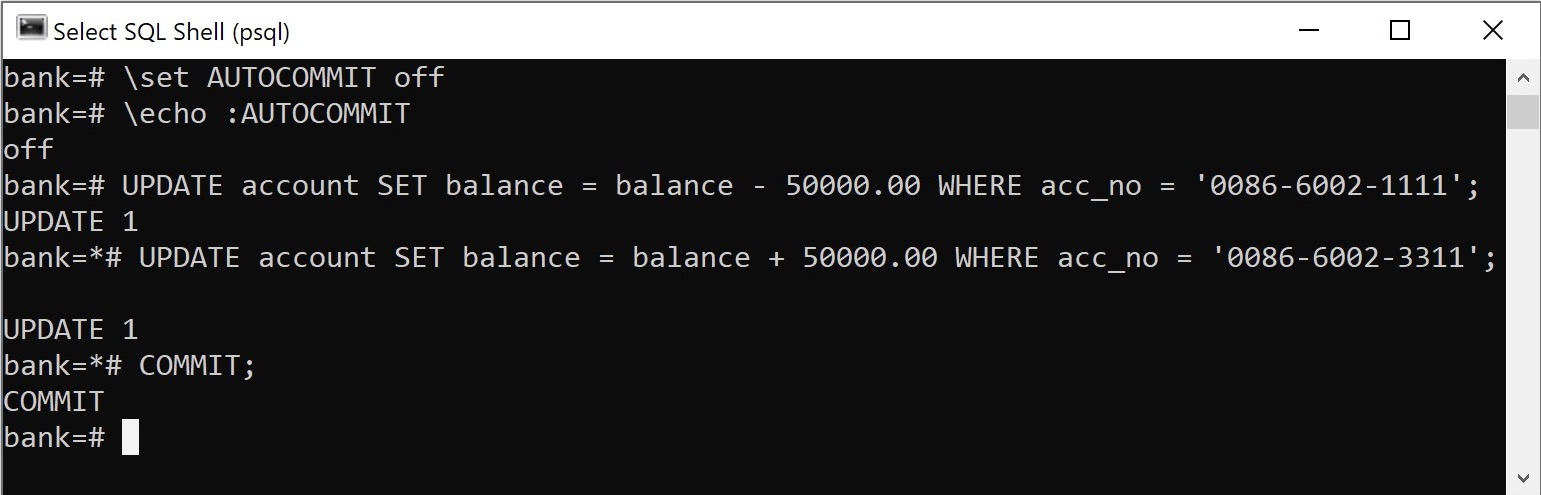
\includegraphics[width=.98\textwidth, trim={0mm 0mm 0mm 1mm},clip]{images/ch12/tx.jpg}};
  \drawshadow{image}
\end{tikzpicture}
\caption{psql မှတစ်ဆင့် transaction တစ်ခု ဖန်တီးအသုံးပြုပုံ} 
\label{fig:tx}
\end{figure}


\begin{figure}[!htb]
\begin{tikzpicture}
  \node[anchor=south west,inner sep=0] (image) at (0,0)
  {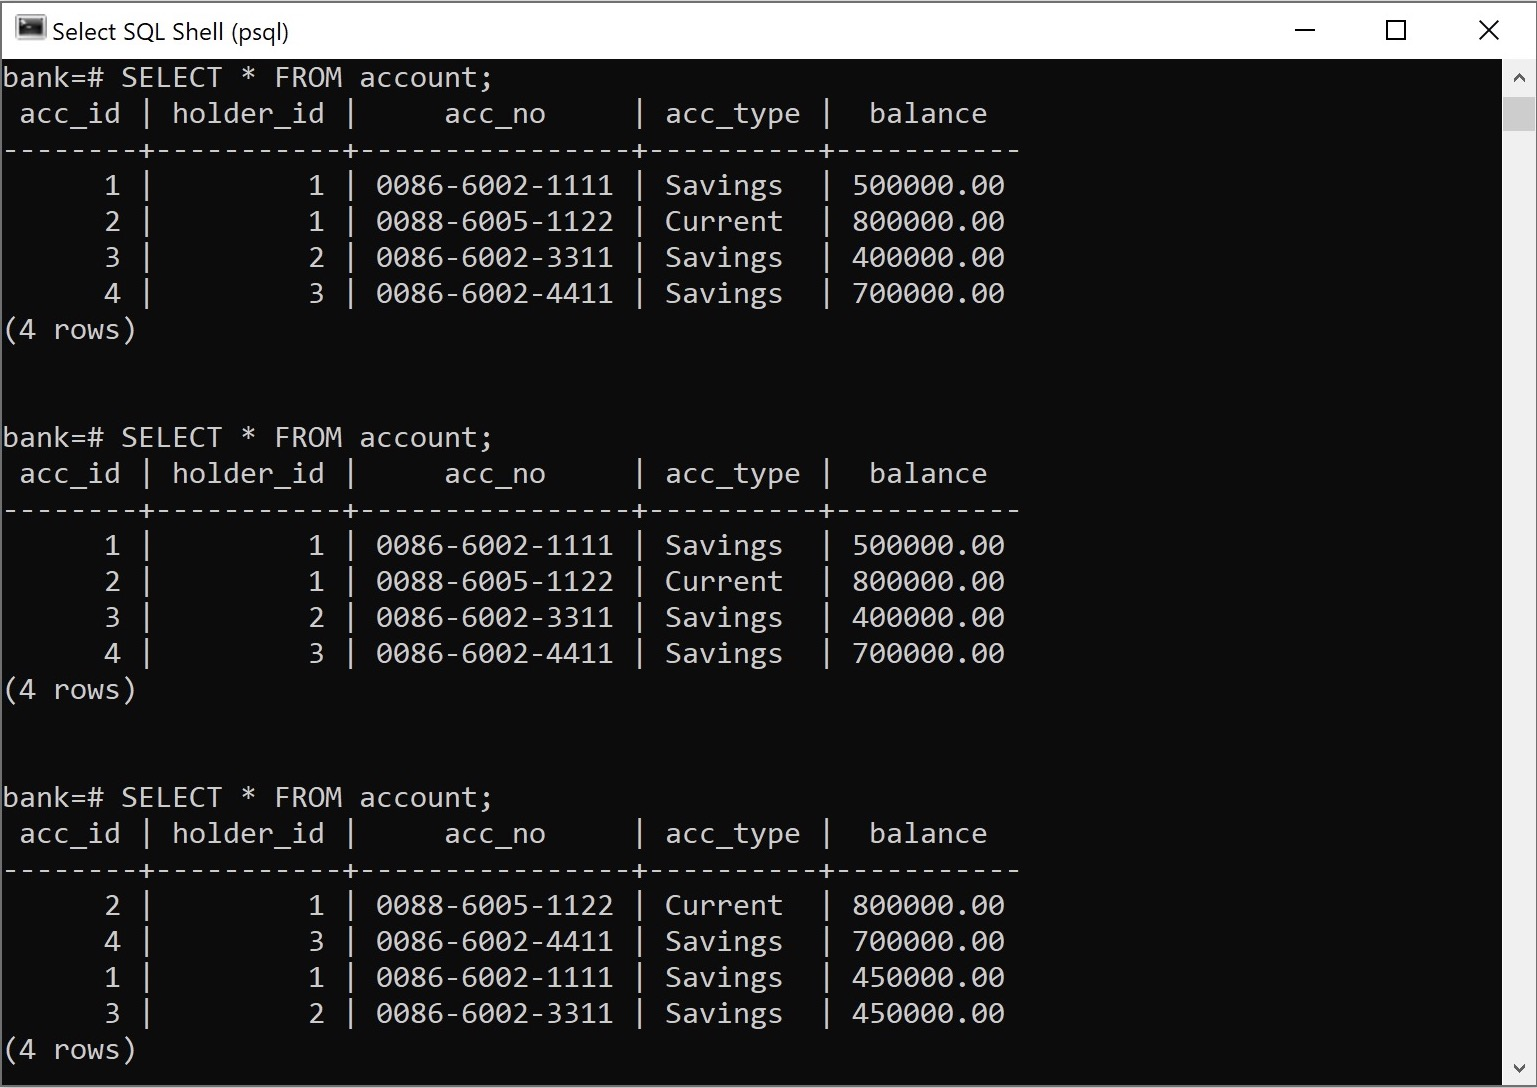
\includegraphics[width=.98\textwidth, trim={0mm 0mm 0mm 1mm},clip]{images/ch12/tx_check.jpg}};
  \drawshadow{image}
\end{tikzpicture}
\caption{အခြား transaction တစ်ခုကို psql မှ စောင့်ကြည့်ပုံ}
\label{fig:txchk}
\end{figure}

\fEn{Psycopg} ဒရိုက်ဗာက သူ့နဂိုအတိုင်းဆိုရင် \fCode{AUTOCOMMIT} ပိတ်ပြီးသားပါ။ ပထမဆုံး \fCode{execute} လုပ်တဲ့အခါ \fEn{transaction} ကို အလိုအလျောက် စပေးပါတယ် (\fCode{execute} လုပ်ပြီဆိုတာနဲ့ \fCode{BEGIN} ကို အရင်လုပ်ပေးမှာပါ)။ \fCode{COMMIT} လုပ်ရင် \fCode{conn.commit()}\fEn{,} \fCode{ROLLBACK} ဆိုရင် \fCode{conn.rollback()} ခေါ်ပေးရပါမယ်။ \fCode{commit()} မလုပ်မိဘဲ ကွန်နက်ရှင် ပိတ်လိုက်ရင် \fEn{transaction} အတွင်း လုပ်ထားသမျှ ဒေတာအပြောင်းအလဲ အားလုံး အတည်မဖြစ်တော့ဘဲ အားလုံး ပျက်ပြယ်သွားပါမယ်။ 

\fEn{Psycopg} နဲ့ \fEn{transaction} စီမံတဲ့ နမူနာပုံစံကို အောက်မှာကြည့်ပါ။ \fEn{Transaction} စီမံတဲ့နေရာမှာ \fEn{exception handling} က အရေးပါပါတယ်။ \fCode{try} ထဲမှာ \fEn{transaction} မှာ ပါဝင်တဲ့ အဆင့်တွေကို လုပ်ဆောင်ရလေ့ရှိတယ်။ အခု ဥပမာမှာ \fEn{update} နှစ်ခု လုပ်ထားတယ်။ နှစ်ခုလုံး ပြဿနာမရှိဘဲ ပြီးရင် \fCode{commit} လုပ်သွားမယ်။ အကြောင်းတစ်ခုခုကြောင့် \fEn{exception} တက်ခဲ့ရင် \fCode{except} ဘလောက်ထဲ ရောက်ပြီး \fCode{rollback} ဖြစ်မှာပါ။
%
\begin{py}
# File: db_transaction_eg1.py
# ß\fEn{Transaction in Python with Psycopg}ß
import psycopg2

conn = psycopg2.connect(dbname="bank", user="postgresql", 
                        password="asdfgh", host="localhost", port="5432")
cur = conn.cursor()

try:
    cur.execute("UPDATE account SET balance = balance - 50000.00 "
                "WHERE acc_no = '0086-6002-1111'")
    cur.execute("UPDATE account SET balance = balance + 50000.00 "
                "WHERE acc_no = '0086-6002-3311'")
    conn.commit()
except psycopg2.Error as e:
    conn.rollback()
    print("Database error: ", e)
except Exception as e:
    conn.rollback()
    print("Unknown error: ", e)
finally:
    cur.close()
    conn.close()
\end{py}
%
\fCode{except} ဘလောက်တွေမှာ \fCode{rollback} လုပ်ဖြစ်အောင် လုပ်ဖို့ သေချာဂရုစိုက်ရပါမယ်၊ မေ့ကျန်ခဲ့တာ ဖြစ်နိုင်တယ်။ ဒီလို မဖြစ်အောင် ကူညီပေးတဲ့ \fCode{with} စတိတ်မန့်ကို ပိုအသုံးများတယ်။ \fEn{Connection} နဲ့ \fEn{cursor} ကို \fCode{with} နဲ့တွဲသုံးရင် \fEn{commit, rollback} နဲ့ \fEn{cursor} ပိတ် ကိစ္စတွေကို အလိုအလျောက် လုပ်ပေးမှာမို့လို့  မေ့ကျန်ခဲ့စရာ အကြောင်း သိပ်မရှိတော့ဘူး။ \fEn{Connection} ကိုပဲ သေချာဂရုစိုက် ပိတ်ပေးဖို့ လိုတယ်။

%
\begin{py}
# File: db_transaction_eg2.py
# ß\fEn{Using}ß with ß\fEn{statement}ß

conn = None
try:
    conn = psycopg2.connect(dbname="bank", user="postgresql", 
                            password="asdfgh", host="localhost", port="5432")
    with conn:
        with conn.cursor() as cur:
            cur.execute("UPDATE account SET balance = balance - 50000.00 "
                        "WHERE acc_no = '0086-6002-1111'")
            cur.execute("UPDATE account SET balance = balance + 50000.00 "
                        "WHERE acc_no = '0086-6002-3311'")
except psycopg2.Error as e:
    print("Database error: ", e)
except Exception as e:
    print("Unknown error: ", e)
finally:
    conn.close()
\end{py}
%


\begin{mytcboxflt}
\fEn{Psycopg} ဗားရှင်း \fEn{2.5} ကစပြီး \fEn{connection, cursor} တို့ကို \fCode{with} စတိတ်မန့်နဲ့ တွဲဖက် အသုံးပြုနိုင်ပါတယ်
%
\begin{pytc}
conn = psycopg2.connect()

with conn:
    with conn.cursor() as cur:
        cur.execute(SQL1)

conn.close()
\end{pytc}
\fEn{Connection} နဲ့ဆိုင်တဲ့ \fCode{with} ဘလောက် \fEn{(outer \fCode{with})} ပြီးဆုံးသွားတယ်၊ \fEn{exception} မဖြစ်ဘူးဆိုရင် \fEn{transaction} ကို \fEn{commit}  လုပ်ပေးမှာဖြစ်ပြီး \fEn{exception} ဖြစ်ခဲ့ရင်တော့ \fEn{rollback} ဖြစ်သွားမှာပါ။ \fEn{Cursor} နဲ့ သက်ဆိုင်တဲ့ \fCode{with} ဘလောက် \fEn{(inner \fCode{with})} ပြီးဆုံးရင် \fEn{cursor} ကို အလိုအလျောက် ပိတ်ပေးမှာဖြစ်ပေမဲ့ \fEn{transaction} က ဆက်ရှိနေအုံးမှာပါ။ \fEn{Transaction commit/rollback} က \fEn{connection} နဲ့ဆိုင်တဲ့ \fCode{with} ဘလောက် အဆုံးမှာ ဖြစ်တာပါ။ \fCode{with} က \fEn{connection} ကို အလိုအလျောက် မပိတ်ပေးပါဘူး။ ဒါကြောင့် ကိုယ်တိုင် ပိတ်ပေးရပါမယ်။
\end{mytcboxflt}
\clearpage


\section{Concurrency}
ဒေတာဘေ့စ်တွေဟာ တစ်ချိန်တည်း \fEn{user} အများအပြား တစ်ပြိုင်နက် အသုံးပြုရင် ဖြစ်ပေါ်နိုင်တဲ့ \fEn{concurrency problem} တွေ မဖြစ်ပေါ်အောင် ကာကွယ်ဖို့အတွက် နည်းလမ်းတွေ ထောက်ပံပေးထားပါတယ်။ \fEnEmp{Concurrency} ဆိုတာ တစ်ခုထက်ပိုတဲ့ အလုပ်တွေ ကွန်ပျူတာက တစ်ချိန်တည်းမှာ လုပ်ဆောင်ပေးနေတာကို ဆိုလိုတာပါ။ တစ်ချိန်တည်း လုပ်ဆောင်ပေးတယ် ဆိုပေမဲ့ အားလုံး တစ်ပြိုင်နက်တည်း လုပ်ဆောင်တာ ဟုတ်ချင်မှ ဟုတ်မှာပါ။ အလုပ်တစ်ခုစီကို အလှည့်ကျ လုပ်ဆောင်ပေးပြီး တစ်ပြိုင်နက်ထဲ ဖြစ်ပျက်နေတယ်လို့ ထင်ရအောင် စီမံထားတာလည်း ဖြစ်နိုင်ပါတယ်။ 

ကလပ်စစ် \fEn{concurrency problem} ဥပမာတစ်ခုကို ဒီအပိုင်းမှာ လေ့လာကြည့်ပါမယ်။ အောက်ဖော်ပြပါ ပရိုဂရမ်ကုဒ် အစိတ်အပိုင်းဟာ ငွေထုတ်ယူတဲ့ ကိစ္စအတွက် ဖြစ်ပါတယ်။
%
\begin{py}
# Step 1: select account balance from database
cur.execute("""
    SELECT balance FROM account WHERE acc_no = %s
""", (acc_no,))
account_balance = cur.fetchone()

# Step 2: check if the balance is enough
if not account_balance:
    raise Exception("Account not found.")
elif account_balance[0] < amount:
    raise Exception("Insufficient funds in the account.")

# Step 3: Debit the account
cur.execute("""
    UPDATE account
    SET balance = balance - %s
    WHERE acc_no = %s
""", (amount, acc_no))
conn.commit()
\end{py}
%

ငွေထုတ်တဲ့ကိစ္စမှာ အကြမ်းဖျဉ်း \fEn{step} သုံးခု ပါဝင်တာ တွေ့ရမှာပါ 
%
\begin{itemize}
    \item လက်ကျန်ငွေ \fEn{select} လုပ်ခြင်း
    \item လက်ကျန်ငွေ လုံလောက်မှု ရှိ/မရှိ စစ်ဆေးခြင်း
    \item လက်ကျန်ငွေ \fEn{update} လုပ်ခြင်း
\end{itemize}
%
(ဒါ့ထက် အသေးစိတ် ထပ်ခွဲလို့ ရအုံးမှာပါ၊ ရှေ့ဆက်ရှင်းပြမဲ့ ကိစ္စအတွက် ဒီလောက်နဲ့က နားလည်ရ ပိုလွယ်ပါမယ်)။

\fEn{Concurrent} ပရိုဂရမ်တစ်ခုဟာ ငွေထုတ်သူ တစ်ဦးချင်းစီအတွက် ဒီ အစဉ်လိုက် \fEn{step} သုံးခုကို လုပ်ဆောင်ပေးရမှာပါ။ တစ်ချိန်တည်း နှစ်ယောက်ထုတ်ရင် \fEn{step} တစ်ခုစီကို တစ်ယောက် တစ်လှည့် နှစ်ယောက်လုံးအတွက် တစ်ချိန်တည်းမှာ ဆောင်ရွက်ပေးရပါမယ်။ အနီးစပ်ဆုံး မြင်သာအောင် ပြောမယ်ဆိုရင်  အဖျော်ဆရာတစ်ယောက် လက်ဖက်ရည်ဖျော်သလိုပဲ၊ တစ်ခွက်ပြီးမှ တစ်ခွက်ဖျော်တာ မဟုတ်ဘူး၊ လက်ဖက်ရည်ခွက်တွေ ရှေ့မှာစီချထားပြီး အကျရည်ထည့်၊ နို့ဆီထည့်၊ နို့စိမ်းထည့် အားလုံး တစ်ပြိုင်တည်းနီးပါး အပြီးဖျော်တာ။ အလုပ်တွေကို တစ်ချိန်တည်း လုပ်တယ်ဆိုတာ ဒီသဘောကို ဆိုလိုတာ။ 

\begin{figure}[!htb]
    \incfig[0.56]{accwithdrawconcur1}
    \caption{ငွေထုတ်ကိစ္စ နှစ်ခု တစ်ချိန်တည်း အလှည့်ကျ လုပ်ဆောင်ပုံ ဖြစ်နိုင်ခြေ ၃ ခု (အားလုံး မဟုတ်ပါ)။ concurrency သဘာဝအရ ဘယ်လို အလှည့်ကျမလဲ ဆိုတာက random ပဲ၊ ပုံသေမရှိဘူး။ ပရိုဂရမ်မာက အလှည့်ကျ အစီအစဉ်ကို လိုသလို ထိန်းကွပ်လို့ မရနိုင်ဘူး။}
    \label{fig:accwithdrawconcur1}
\end{figure}



အဖျော်ဆရာ အလုပ်လုပ်ပုံနဲ့ \fEn{concurrent} ပရိုဂရမ် လုံးဝမတူတဲ့ အချက်တစ်ခုရှိတယ်။ \fEn{Concurrency} သဘာဝအရ အလုပ်တစ်ခုစီကို အချိန်အနည်းငယ်ကြာ အလှည့်ကျ လုပ်ဆောင်ပေးပါတယ်။ ဒီလို အလှည့်ပေးစနစ်ကို \fEn{operating system} မှာ ပါဝင်တဲ့ \fEn{scheduler} က  စီမံတာဖြစ်ပြီး ပရိုဂရမ်ရေးသားသူ လိုသလို စိတ်ကြိုက် ထိန်းကွပ်လို့ မရနိုင်ပါဘူး။ ဒီအတွက်ကြောင့် အလုပ်နှစ်ခုမှာပါဝင်တဲ့ \fEn{step} တွေ ဘယ်လိုအစဉ်နဲ့ အလှည့်ကျ လုပ်ဆောင်မလဲ ပုံသေတွက်လို့မရတော့ဘူး။  



ပုံ (\fRefNo{\ref{fig:accwithdrawconcur1}}) မှာ အလုပ်နှစ်ခု အလှည့်ကျ လုပ်ဆောင်ပုံ ဖြစ်နိုင်ခြေ သုံးခုကို တွေ့ရပါမယ်။ အလုပ်နှစ်ခုကို အထက်အောက် အရောင်ခွဲ ပြထားတယ်။ စတုဂံငယ် တစ်ခုစီက ပါဝင်တဲ့ \fEn{step} တစ်ခုချင်းကို ကိုယ်စားပြုတာ၊ မြှားဟာ အချိန် စီးဆင်းရာ။ ပုံမှာပြထားတာ သုံးခုအပြင် အခြား ဖြစ်နိုင်တဲ့ အစီအစဉ်တွေ ကျန်ပါသေးတယ်။ သင်္ချာနည်းနည်းကျွမ်းတယ်၊ စိတ်ဝင်စားတယ်ဆိုရင် ဖြစ်နိုင်ခြေ အားလုံး တွက်ကြည့်လို့ရပါတယ် (\fEnEmp{Permutations with repetition} \fEn{or} \fEnEmp{combinatorics} သဘောတရားနဲ့ တွက်ရမှာပါ၊ အခုကိစ္စအတွက် ဖြစ်နိုင်ခြေ အားလုံး အခု ၂၀ ရှိပါမယ်)။




\fEn{Concurrent} အလုပ်တွေကြားမှာ အချက်အလက် မျှဝေသုံးစွဲတာ မရှိရင် ထူးထူးခြားခြား ပြဿနာ မရှိပါဘူး၊ ပရိုဂရမ် ရေးသားရတာလည်း ပုံမှန်ထက် အများကြီး မခက်ဘူး။ ဒါပေမဲ့ အချက်အလက် မျှဝေသုံးစွဲတာ ရှိခဲ့ရင်တော့ ပြဿနာရှိလာပါတယ်။ ဥပမာ အကောင့်တစ်ခုတည်းကနေ တစ်ပြိုင်တည်း ငွေထုတ်တဲ့ ဖြစ်စဉ်ကို စဉ်းစားကြည့်ပါ။ စန္ဒီနဲ့ ကေသီ နှစ်ယောက်ပေါင်း အကောင့်တစ်ခု ဖွင့်ထားတယ်။ လက်ရှိ အကောင့် လက်ကျန်ငွေ  ၅ သိန်း ရှိပြီး သူတို့ နှစ်ယောက် တစ်နေရာစီကနေ ၄ သိန်း သီးခြား ထုတ်ယူကြတာ တိုက်တိုက်ဆိုင်ဆိုင် တစ်ချိန်တည်းဖြစ်သွားတယ်လို့ စိတ်ကူးကြည့်ပါ။ ဒီဖြစ်စဉ်မှာ အကောင့် \fEn{record} ဟာ \fEn{shared data} ဖြစ်ပြီး အလုပ်နှစ်ခုက တူညီတဲ့ \fEn{record} တစ်ခုတည်းကို တစ်ချိန်တည်းမှာ \fEn{update} လုပ်ဖို့အတွက် ကြိုးစားကြတာကို တွေ့ရမှာပါ။

% (တစ်ယောက် ၄ သိန်း ထုတ်ယူမှာ)။ အကောင့်ထဲ ရှိတာမှ နှစ်ယောက်ပေါင်း ၅ သိန်းပဲ ရှိတဲ့အတွက် ၈ သိန်းထုတ်လို့ ဘယ်နည်းနဲ့မှ မရသင့်ပါဘူး။ %\fEn{Concurrent} ပရိုဂရမ် တည်ဆောက်ရတာကလည်း အများကြီး ရှုပ်ထွေးခက်ခဲလာနိုင်တယ်။ စဉ်းစားတာ တစ်ချက်လေး မှားသွားတာနဲ့  ... (\fEn{Concurrency} မှာ အားသာချက်/အားနည်းချက် အမျိုးမျိုး ရှိပါတယ်၊ အခန်း (\fRefNo{\ref{ch:concurrency}}) မှာ ဆက်လက် ဖော်ပြပေးမှာပါ)။   

%
\begin{figure}[!htb]
    \incfig[0.6]{accwithdrawconcur2}
    \caption{Concurrency problem ဥပမာ။ ၅ သိန်းရှိတဲ့ အကောင့် တစ်ခုတည်းကနေ တစ်ယောက် ၄ သိန်း၊ နှစ်ယောက် တစ်ချိန်တည်း ငွေထုတ်တဲ့အခါ step တစ်ခုချင်းအလိုက် လက်ကျန်ငွေ ပြောင်းလဲပုံ}
    \label{fig:accwithdrawconcur2}
\end{figure}
%

ပုံ (\fRefNo{\ref{fig:accwithdrawconcur1}}) အပေါ်ဆုံးကအတိုင်း အလှည့်ကျ လုပ်ဆောင်တယ် ဆိုပါစို့။ \fEn{Step} တစ်ခုချင်းအလိုက် လက်ကျန်ငွေ \fEn{balance} ပြောင်းလဲပုံကို ပုံ (\fRefNo{\ref{fig:accwithdrawconcur2}}) မှာ ပြထားတယ်။ $K_1, K_2, K_3, S_1, S_2, S_3$ တို့ဟာ ကေသီနဲ့ စန္ဒီ့အတွက် \fEn{step} သုံးခုစီလို့ ယူဆပါ \fEn{($K$ for Kathy, $S$ for Sandy)}။ $S_1, K_1, K_2, S_2$ လုပ်ဆောင်ပြီးချိန်အထိ လက်ကျန်ငွေ ၅ သိန်းဟာ နဂိုအတိုင်း မပြောင်းလဲသေးဘူး။



% အပေါ်တန်း စတုဂံ အသေးလေးတွေဟာ ကေသီငွေထုတ်တာ၊ အောက်ဖက်က စန္ဒီလို့ ယူဆပါ။ အပေါ်ဆုံး အလှည့်ကျ ပုံစံအရ $S_1, K_1, K_2, S_2, K_3, S_3$ အစဉ်နဲ့ လုပ်ဆောင်မှာပါ ($S$ နဲ့ $K$ ဟာ စန္ဒီနဲ့ ကေသီကို ကိုယ်စားပြုတာ)။  \fEn{Step} တစ်ခုချင်း ဖြစ်ပျက်တာကို လေ့လာကြည့်ရင် ပုံ (\fRefNo{\ref{fig:accwithdrawconcur2}})

$K_3$ အပြီးမှာ လက်ကျန်ငွေ \fEn{balance} ဟာ ၁ သိန်း ဖြစ်သွားပြီ။ ဒီအတိုင်းဆိုရင် နောက်\allowbreak ထပ် ၄ သိန်း ထုတ်လို့ မရသင့်တော့ဘူး။ $S_2$ မှာ လက်ကျန်ငွေ လောက်/မလောက် စစ်ခဲ့ချိန်က ဒီလိုမဟုတ်သေးဘူး၊ အဲ့တုန်းက ၅ သိန်းရှိခဲ့တာ။ ဆိုတော့ $S_2$ အရဆိုရင် $S_3$ ကို ဆက်လက်လုပ်ဆောင်ရမှာပဲ။ $S_3$ ပြီးသွားတဲ့အခါ \fEn{balance} ဟာ အနှုတ် ၃ သိန်းဖြစ်သွားပါတယ်။ ကေသီနဲ့ အေမီဟာ သူတို့မှာ ရှိတဲ့ငွေထက် ဘဏ်ကနေ ၃ သိန်း အပိုထုတ်လို့ရသွားတာ ဖြစ်ပါတယ်။  ပုံ (\fRefNo{\ref{fig:accwithdrawconcur1}}) က နောက်ထပ် ဖြစ်နိုင်ခြေ နှစ်ခုမှာလည်း ဒီပြဿနာ တွေ့ရမှာပါ။

ဘာ့ကြောင့် ဒီလို ဖြစ်ရတာလဲ၊ မဖြစ်အောင် ဘယ်လို ကာကွယ်ရမလဲ။ တစ်ချိန်တည်းမှာ ထုတ်ယူကြပေမဲ့ အကောင့်တစ်ခုတည်းကနေ မဟုတ်ရင်  ဒီလိုပြဿနာ မဖြစ်နိုင်ဘူး။ တစ်နည်းအားဖြင့် မတူညီတဲ့ သီးခြားအကောင့်တစ်ခုစီကနေ တစ်ပြိုင်နက် ငွေထုတ်ယူတာဟာ \fEn{concurrency problem} မဖြစ်စေနိုင်ဘူး။ တစ်ချိန်တည်း၊ အကောင့်တစ်ခုတည်းကနေ ငွေထုတ်တဲ့ကိစ္စနှစ်ခု တိုက်ဆိုင်တဲ့အခါ \fEn{concurrency problem} ရှိနိုင်တာပါ။ ဖြေရှင်းဖို့ နည်းလမ်းကတော့ အကောင့်တစ်ခုကို တစ်ချိန်တည်းမှာ အလုပ်တစ်ခုကပဲ \fEn{update} လုပ်လို့ရအောင် ကာကွယ်ပေးထားရပါမယ်။ \fEn{Transaction} တစ်ခုဟာ ၎င်း \fEn{update} လုပ်ဖို့ ရည်ရွယ်တဲ့ \fEn{record} ကို အခြား \fEn{transaction} တွေကနေ \fEn{update} လုပ်လို့မရအောင် \fCode{FOR UPDATE} နဲ့ တားဆီးနိုင်ပါတယ်။ \fCode{SELECT} လုပ်တဲ့အချိန်မှာ အခုလို တွဲသုံးရမှာပါ    
% အလုပ်နှစ်ခုက \fEn{row} တစ်ခုတည်းကို တစ်ချိန်တည်းမှာ \fEn{update} လုပ်တာဟာ ဒီပြဿနာရဲ့ အဓိက အကြောင်းအရင်း ဖြစ်တယ်။   
%\fEn{Select} လုပ်တဲ့ \fEn{Record locking}  ဒီလိုမဖြစ်အောင် ကာကွယ်တဲ့ နည်းလမ်းတစ်ခုက \fEn{} \fEn{update} လုပ်ဖို့ ရည်ရွယ်ချက်နဲ့ \fEn{select} အကောင့် \fEn{record} ကို \fEn{lock} လုပ်တာ။  
%
\begin{py}
# File: db_transaction_and_concurrency.py

# Step 1: select account balance from database
cur.execute("""
    SELECT balance FROM account WHERE acc_no = %s FOR UPDATE
""", (acc_no,))
account_balance = cur.fetchone()
\end{py}
% 
\fEn{Concurrency} စကားနဲ့ ပြောရင် \fCode{FOR UPDATE} ဟာ \fEn{select} လုပ်လိုက်တဲ့ \fEn{row} တွေအပေါ်မှာ \fEn{exclusive lock} ရယူတာဖြစ်တယ်။ ဒါနဲ့ပါတ်သက်တဲ့ အသေးစိတ်ကို \fEn{concurrency} အခန်းမှာ သီးခြားရှင်းပြမှာပါ။ 

\fEn{Concurrency} ဟာ ကျယ်ပြန့်ပြီး သီးခြားအထူးပြု လေ့လာရမဲ့ အပိုင်းဖြစ်ပါတယ်။ စာမျက်နှာ \fRefNo{\pageref{ch:concurrency}} အခန်း (\fRefNo{\ref{ch:concurrency}}) မှာ အခြေခံ \fEn{concurrency} အကြောင်း ဖော်ပြပေးထားတယ်။ အခု တွေ့ခဲ့ရတဲ့ ဥပမာက ဒေတာဘေ့စ် အပ်ပလီကေးရှင်းတွေမှာ ကြုံတွေ့ရနိုင်တဲ့ \fEn{concurrency problem} တွေ အများကြီးထဲကမှ အခြေခံ တစ်ခုလေးပဲ ရွေးထုတ်ထားတာ။ ဒေတာဘေ့စ် \fEn{concurrency} နဲ့ ပါတ်သက်ပြီး ပေးထားတဲ့ ကိုးကားစာအုပ်တွေ၊ ဒါမှမဟုတ် အခြား တစ်နေရာကနေ ဖြည့်စွက်လေ့လာဖို့ တိုက်တွန်းပါတယ်။ 

\section{SQL Injection and Dynamic SQL}
\fEn{String interpolation} နည်းလမ်းနဲ့ \fEn{Dynamic SQL} မထုတ်သင့်ဘူး ပြောခဲ့ပေမဲ့ ဘာ့ကြောင့်လဲ အကြောင်းအရင်းကို မရှင်းပြခဲ့ဘူး။ ဒါနဲ့ ပါတ်သက်ပြီး အကြောင်းအချက် တချို့ကို ဆက်လက် လေ့လာကြပါမယ်။ အသိသာဆုံး ပြဿနာတစ်ခုက \fEn{SQL} နဲ့ \fEn{Python} တို့ဟာ \fEn{string} ကို ဖော်ပြပုံ မတူတာပါ။ နောက်ဆုံးအမည် \fCode{O'Brian} နဲ့ အကောင့်ပိုင်ရှင်ကို \fEn{SQL} မှာ အခုလို \fEn{select} လုပ်ရပါတယ်။ 

%
\begin{sql}
SELECT * FROM account_holder WHERE lname = 'O''Brian';
\end{sql}
%
စာသားကို \fEn{single quote} နှစ်ခုအတွင်းမှာ ရေးတယ်။ စာသားထဲမှာ \fCode{'} ပါနေရင် \fCode{''} (\fEn{single quote} နှစ်ခု) နဲ့ \fEn{escape} လုပ်ပေးရပါမယ်။ 

\fEn{SQL identifier} တွေမှာ စပေ့စ်၊ ဟိုက်ဖန် (သို့) အခြား ထူးခြားသင်္ကေတတွေ ပါဝင်နေတဲ့အခါ \fEn{double quotes} \fEn{(\mintinline{text}|"|)}  နှစ်ခုအတွင်း ထည့်ရေးလေ့ရှိပါတယ်။ \fEn{Identifier} က \fEn{SQL reserved keyword} ဖြစ်နေရင်လည်း အလားတူပဲ \fEn{double quotes} သုံးရတယ်။ (မှတ်ချက်။\qquad ။ \fEn{Identifier} ဆိုတာ \fEn{table, column, function, variable} စတာတွေရဲ့ နံမည်ကို ဆိုလိုတာပါ)။

%
\begin{sql}
-- # ß\fEn{and}ß - ß\fEn{are special characters}ß
SELECT fname "#1st-name" FROM account_holder;
-- ß\fEn{contains space in the column alias}ß
SELECT concat(fname, ' ', lname) "Full Name" FROM account_holder;
-- order ß\fEn{is one of the reserved keywords}ß
CREATE TABLE "order" (
    id SERIAL PRIMARY KEY
);
\end{sql}
%
\fEn{Identifier} ထဲမှာ \fCode{"} ပါနေရင် \fCode{""} (\fEn{double quote} နှစ်ခု) နဲ့ \fEn{escape} လုပ်ရပါမယ်။
%
\begin{sql}
-- ß\fEn{Column alias contains double quotes,} Students(only "Best")ß
SELECT name "Students(only ""Best"")" FROM student 
WHERE grade = 'A' OR grade = 'A+';
\end{sql}
%

အောက်မှာ ရေးထားတဲ့အတိုင်း စမ်းကြည့်ရင် \fEn{SQL} ဆင်းတက်စ်အယ်ရာ ဖြစ်မှာပါ။ နံမည်မှာပါတဲ့ \fCode{'} ကို \fCode{''} ပြောင်းပေးဖို့ လိုတာက တစ်ကြောင်း၊ နောက်တစ်ချက်က နံမည်ဟာ စာသားဖြစ်တဲ့အတွက် \fEn{SQL} ထဲမှာ \fCode{'O''Brian'} ဖြစ်ရပါမယ်။ အခုလို ဆက်ထားရင်
%
\begin{py}
# File: db_problem_of_str_interpolation.py
last_name = "O'Brian"
# this will cause SQL syntax error!!!
cur.execute("SELECT * FROM account_holder WHERE lname = " + last_name)
\end{py}
%
\fEn{SQL string} က 
%
\begin{py}
"SELECT * FROM account_holder WHERE lname = O'Brian"
\end{py}
%
ဖြစ်နေတာကြောင့် ဆင်းတက်စ်မမှန်ဘူး။ အမှန်ဖြစ်အောင်က ဒီလို ဆက်ရမှာပါ

%
\begin{py}
cur.execute("SELECT * FROM account_holder "
            "WHERE lname = '" + last_name.replace("'", "''") + "'")
\end{py}
%

\fEn{SQL} ကုဒ်ထဲမှာ \fEn{string} က \fEn{dynamic} အပိုင်းဖြစ်နေတဲ့အခါ မမှားအောင် ဂရုစိုက်ရပြီး အတော်လေး ကရိကထများတယ်။ \fEn{Identifier} တွေက \fEn{dynamic} ဖြစ်နေတယ်၊ \fEn{double quote} လုပ်ရမဲ့ဟာ ဖြစ်နေရင်လည်း အလားတူပြဿနာမျိုး ကြုံရမှာပါ။ ရှေ့ပိုင်းမှာ ဖော်ပြခဲ့တဲ့ နည်းတွေက ဒီလိုကိစ္စတွေကို ကြိုတင်စဉ်းစား ဖြေရှင်းပေးထားတာမို့လို့ ပရိုဂရမ်မာ သိပ်ခေါင်းစားစရာ မလိုတော့ဘူး
%
\begin{py}
cur.execute("SELECT * FROM account_holder WHERE lname = %s", (last_name,))
\end{py}
%
\mintinline{text}|%s| နေရာမှာ အစားထိုးပြီး ရမဲ့ \fEn{SQL} ကို \fCode{mogrify} ဖန်ရှင်သုံးပြီး ထုတ်ကြည့်ပါ
%
\begin{py}
sql_full = cur.mogrify("SELECT * FROM account_holder "
                       "WHERE lname = %s", (last_name,))
print(sql_full.decode('utf-8'))
\end{py}
%
ဖြစ်သင့်တဲ့အတိုင်း \fEn{SQL} အမှန် တွေ့ရပါလိမ့်မယ်
%
\begin{codetxt}
SELECT * FROM account_holder WHERE lname = 'O''Brian'
\end{codetxt}
%

\subsection*{SQL Injection}
\fEn{Dynamic SQL} ကို \fEn{string interpolation} နည်းတွေနဲ့ ထုတ်တဲ့အခါ ရှေ့မှာဖော်ပြခဲ့တဲ့ အခက်အခဲတွေအပြင် ပိုပြီး နက်ရှိုင်းတဲ့ ပြဿနာတစ်ခု ကြုံရနိုင်ပါတယ်။ အဲ့ဒါကတော့ \fEn{SQL Injection} လို့ခေါ်တဲ့ နည်းလမ်းတစ်မျိုးနဲ့ ဒေတာဘေ့စ် စီကျူရတီပိုင်း တိုက်ခိုက် ခံရနိုင်ခြင်းပါပဲ။ \fEn{SQL Injection} ဆိုတာ ၎င်းလုပ်ဆောင်စေချင်တဲ့ \fEn{SQL} ကုဒ်တွေကို ဟက်ကာက ပရိုဂရမ် \fEn{input} ကနေတစ်ဆင့် ထည့်သွင်းတဲ့ နည်းလမ်းလို့ အကြမ်းဖျဉ်း ယူဆနိုင်တယ်။

အောက်ပါ ပရိုဂရမ်ကုဒ် ကောက်နုတ်ချက်မှာ အသုံးပြုသူ \fEn{user} က \fCode{last\_name} ကို \fEn{input} ထည့်ပေးမယ်လို့ ယူဆပါ။ \fEn{SQL} နားလည်ကျွမ်းကျင်တဲ့ ဟက်ကာဟာ သူ့ရဲ့ အကောင့် လက်ကျန်ငွေစာရင်းကို \fEn{update} ဖြစ်သွားစေမဲ့ \fEn{input string} ကို မှန်းဆနိုင်ပါတယ်။  
%
\begin{py}
# File: db_sql_inj1.py 

# ß\fEn{SQL injection example}ß
# ß\fMM{ဒီအတိုင်း ထည့်ပေးမယ်လို့ ယူဆပါ}ß
last_name = input("Enter last name: ")
sql = ("SELECT * FROM account_holder "
       "WHERE lname = '") + last_name + "'"
print(sql)
cur.execute(sql)
\end{py}
%
\fEn{Input} ကို အခုလို ထည့်လိုက်မယ် ဆိုပါစို့ 
\begin{codetxt}
'; UPDATE account SET balance = 10000000.00 WHERE acc_id = 1;--
\end{codetxt}

ဒီလိုသာဆိုရင် ဟက်ကာဟာ သူ့ရဲ့အကောင့်မှာ $10000000.00$ ရသွားပါပြီ \fEn{(!)}။ သူ့ \fEn{input} ကြောင့် \fEn{SQL} က အခုလို
\begin{sql}
SELECT * FROM account_holder WHERE lname = '';
UPDATE account SET balance = 10000000.00 WHERE acc_id = 1;--'
\end{sql}
ဖြစ်သွားတာ တွေ့ရမှာပါ။ နဂိုရည်ရွယ်တာက အကောင့်ပိုင်ရှင်ကို \fEn{last name} နဲ့ ရှာဖို့ပေမဲ့ ဟက်ကာရဲ့ \fEn{input} ကြောင့် \fEn{update} လုပ်တဲ့ \fEn{SQL} ပါ တွဲရက် ပါသွားတယ်။ အဆုံးမှာ \fCode{--'} ကို သတိပြုပါ။ \fCode{--} ဟာ \fEn{SQL} ကွန်းမန့်ဖြစ်တဲ့အတွက် နောက်မှာ ဘာပဲရှိရှိ အရေးမကြီးတော့ဘူး (နောက်ဆုံး \fEn{single quote} ကို အယ်ရာ မဖြစ်အောင် ကွန်းမန့်ပါ ပိတ်ပေးလိုက်တာ)။ တကယ့်လက်တွေ့မှာ \fEn{SQL Injection} ဟာ ဒီ့ထက် ရှုပ်ထွေခက်ခဲကောင်း ခက်ခဲနိုင်ပေမဲ့ အခုဥပမာကနေ အခြေခံ သဘောတရား နားလည်နိုင်မယ် မျှော်လင့်ပါတယ်။

\fEn{SQL injection} ကြောင့် ကတ်စတမ်မာ ကိုယ်ရေးကိုယ်တာ အချက်အလက်တွေ ပေါက်ကြားကုန်နိုင်ပါတယ်။ ရက်စွဲအလိုက် ငွေဝင်ငွေထွက်စာရင်း စစ်လို့ရတယ် ယူဆပါ။ ရက်စွဲကို အောက်ပါအတိုင်း ထည့်ပေးလိုက်ရင် ဟက်ကာဟာ အခြားသူ စာရင်းတွေကိုပါ ကြည့်လို့ရသွားပါမယ်။ 
%
\begin{py}
# File: db_sql_inj1.py 

acc_id = 1

txn_date = "2024-08-01' OR 1 = 1 --"
sql = ("SELECT * FROM account_transaction WHERE date(txn_date) = '" 
       + txn_date + "' AND acc_id = " + str(acc_id))
print(sql)
cur.execute(sql)
transactions = cur.fetchall()

for tx in transactions:
    print(tx)
\end{py}
%
ထွက်လာတဲ့ \fEn{SQL} ကို ကြည့်တဲ့အခါ
\begin{sql}
SELECT * FROM account_transaction 
WHERE date(txn_date) = '2024-08-01' OR 1 = 1 --' AND acc_id = 1
\end{sql}
\fCode{1 = 1} က \fEn{true} ဖြစ်မယ်။ ဒီတော့ \fCode{OR} သုံးထားတဲ့ \fCode{WHERE} ကွန်ဒီရှင်တစ်ခုလုံးကလည်း ဘယ်တော့မဆို \fEn{true} ဖြစ်နေမှာပါ။ နောက်ပိုင်းက ကွန်းမန့်ဖြစ်သွားတော့ \fCode{AND acc\_id = 1} ကလည်း ထူးခြားမှု မရှိတော့ဘူး။ ဒါကြောင့် အကျိုးသက်ရောက်မှုအရ \fCode{WHERE} မပါဘဲ \fEn{table} တစ်ခုလုံး \fEn{select} လုပ်တာနဲ့ တူတူဖြစ်သွားမှာပါ
\begin{sql}
SELECT * FROM account_transaction WHERE true;
-- ß\fEn{, which is effectly the same as below:}ß
SELECT * FROM account_transaction;
\end{sql}

အခုတွေ့ခဲ့ရတဲ့ ဥပမာမျိုးတွေဟာ ဘဏ်လုပ်ငန်းလို ကုမ္ပဏီကြီးတွေအတွက်ဆိုရင် အတော်ကို ပြဿ\allowbreak နာကြီးတဲ့ စီကျူရတီ ကျိုးပေါက်မှု ဖြစ်ပါလိမ့်မယ်။ တရားစွဲဆို ခံရတာ ဖြစ်နိုင်တယ်။ ကတ်စတမ်မာတွေ လက်လွှတ်ဆုံးရှုံးရနိုင်တယ်။ \fEn{SQL injection} နဲ့ပါတ်သက်လို့ လုံးဝ ပေါ့ဆလို့မရဘူး၊ အထူးဂရုစိုက်ဖို့ လိုမယ်ဆိုတာ ဒီလောက်ဆိုရင်  သဘောပေါက်မယ် ထင်ပါတယ်။ 

\section*{ဖတ်ရှုလေ့လာသင့်သည့် စာအုပ်များနှင့် အခြား အရင်းအမြစ်များ}
\noindent
\fEn{1. \textbf{Viescas, J. L.} \textit{SQL Queries for Mere Mortals, 4\textsuperscript{th} Edition}. Addison-Wesley, 2018. }\\
\noindent
\fEn{2. \textbf{Hernandez M. J.} \textit{Database Design for Mere Mortals, 4\textsuperscript{th} Edition}. Addison-Wesley, 2021. }\\
\noindent
\fEn{3. \textbf{Connolly T. M., Begg C. E.} \textit{Database Systems: A Practical Approach to Design, Implementation, and Management, 6\textsuperscript{th} Edition}. Pearson, 2015. }\\
\noindent
\fEn{4. \textbf{Silberschatz A., Korth H. F., Sudarshan S.} \textit{Database
System Concepts, 7\textsuperscript{th} Edition}. McGraw-Hill, 2020. }\\

\subsection*{YouTube Tutorials}
\noindent
\fEn{1. \textbf{techTFQ.} \textit{Learn Complete SQL (Beginner to Advance)}}
\begin{vbtm}
https://www.youtube.com/playlist?list=PLavw5C92dz9Ef4E-1Zi9KfCTXS_IN8gXZ
\end{vbtm}
\noindent
\fEn{Tutorial} က \fEn{table} နဲ့ \fEn{sample data SQL script} တွေကို ဖန်တီးသူရဲ့ \fEn{blog page} မှာ \fEn{download} လုပ်လို့ရပါတယ်
\begin{vbtm}
https://techtfq.com/blog/sql-basics-tutorial-for-beginners
\end{vbtm}






% \noindent
% 1. \textbf{Knuth, D. E.} \textit{The Art of Computer Programming, Volume 1: Fundamental Algorithms}. Addison-Wesley, 1968. \\
% (This foundational book on algorithms covers a wide range of computer science topics, from basic concepts to advanced techniques.)
% 
% \noindent
% 2. \textbf{Abelson, H., \& Sussman, G. J.} \textit{Structure and Interpretation of Computer Programs}. MIT Press, 1996. \\
% (A classic introduction to computer programming using Scheme, focusing on the role of computation in systems design.)





% https://castel.dev/post/lecture-notes-2/#code
% https://tex.stackexchange.com/questions/401201/difference-between-align-and-alignedt
